% This must be in the first 5 lines to tell arXiv to use pdfLaTeX, which is strongly recommended.
\pdfoutput=1
% In particular, the hyperref package requires pdfLaTeX in order to break URLs across lines.

\documentclass[11pt]{article}

% Remove the "review" option to generate the final version.
%\usepackage[review]{acl}
\usepackage{acl}

% Standard package includes
\usepackage{times}
\usepackage{latexsym}

% For proper rendering and hyphenation of words containing Latin characters (including in bib files)
\usepackage[T1]{fontenc}
% For Vietnamese characters
% \usepackage[T5]{fontenc}
% See https://www.latex-project.org/help/documentation/encguide.pdf for other character sets

% This assumes your files are encoded as UTF8
\usepackage[utf8]{inputenc}

% This is not strictly necessary, and may be commented out,
% but it will improve the layout of the manuscript,
% and will typically save some space.
\usepackage{microtype}

% <mzhao>
\usepackage{soul}
\usepackage{xspace}
\usepackage{multirow}
\usepackage{amsmath}
\usepackage{amssymb}
\usepackage{bbding}
\usepackage{graphicx}
\usepackage{textcomp}
\usepackage{pifont}
\usepackage[caption=false]{subfig}
\DeclareMathOperator*{\argmax}{arg\,max}
\DeclareMathOperator*{\argmin}{arg\,min}
\def\tasksymbol{$\mathcal{T\mkern-5mu}$\xspace}
\def\md{LMTurk\xspace}
\def\mdr{LMTurker\xspace}
\def\mdrs{LMTurkers\xspace}
\usepackage{xcolor}
\definecolor{blue}{HTML}{4466A5}
\definecolor{green}{HTML}{4E9E5E}
\definecolor{orange}{HTML}{D87B4D}
% </mzhao>

% <cis commands>
\def\figref#1{Figure~\ref{fig:#1}}
\def\figlabel#1{\label{fig:#1}\label{p:#1}}
\def\chapref#1{Chapter~\ref{chap:#1}}
\def\chaplabel#1{\label{chap:#1}\label{p:#1}}
\def\Tabref#1{Table~\ref{tab:#1}}
\def\tabref#1{Table~\ref{tab:#1}}
\def\tabsref#1{Tables~\ref{tab:#1}}
\def\tabrefbare#1{\ref{tab:#1}}
\def\tablabel#1{\label{tab:#1}\label{p:#1}}
\def\Secref#1{\S\ref{sec:#1}}
\def\secref#1{\S\ref{sec:#1}}
\def\seclabel#1{\label{sec:#1}}
\def\qref#1{Eq.~\ref{eqn:#1}}
\def\eqrefn#1{\ref{eqn:#1}}
\def\eqsref#1#2{Eqs.~\ref{eqn:#1}/\ref{eqn:#2}}
\def\eqlabel#1{\label{eqn:#1}}
\def\subsp#1{P_{\mbox{{\scriptsize\rm #1}}}}

\newcounter{notecounter}
\newcommand{\enotesoff}{\long\gdef\enote##1##2{}}
\newcommand{\enoteson}{\long\gdef\enote##1##2{{
\stepcounter{notecounter}
{\large\bf \hspace{1cm}\arabic{notecounter} $<<<$ ##1: ##2 $>>>$\hspace{1cm}}}}}
\enoteson
\enotesoff
% </cis commands>
\newcommand{\mf}[1]{{\color{magenta}#1}}
%\newcommand{\MF}[1]{{\bf{\color{magenta}MF: #1}}}
\newcommand{\MF}[1]{}


% If the title and author information does not fit in the area allocated, uncomment the following
%
%\setlength\titlebox{<dim>}
%
% and set <dim> to something 5cm or larger.


\title{LMTurk: Few-Shot Learners as Crowdsourcing Workers in
  a Language-Model-as-a-Service Framework}

\author{
  Mengjie Zhao\textsuperscript{†}
  \ \ Fei Mi\textsuperscript{‡}
  \ \ Yasheng Wang\textsuperscript{‡}
  \ \ {\bf Minglei Li\textsuperscript{\normalfont{*}}}\\
  {\bf Xin Jiang\textsuperscript{‡}}
  \ \ {\bf Qun Liu\textsuperscript{‡}}
  \ \ {\bf Hinrich Sch\"{u}tze\textsuperscript{†}}\\
  \textsuperscript{†}CIS, LMU Munich
  \ \ \textsuperscript{‡}Huawei Noah's Ark Lab
  \ \ \textsuperscript{*}Huawei Technologies Co., Ltd.\\
  {\tt {\small mzhao@cis.lmu.de,}}
  {\tt {\small \{mifei2,wangyasheng,jiang.xin,qun.liu\}@huawei.com}}
}


%\hypersetup{draft}

\begin{document}
\maketitle

\begin{abstract}
  Vast efforts have been devoted to
  creating high-performance few-shot learners, i.e.,
  large-scale pretrained language models (PLMs)
  that perform well 
  with little downstream task training data.
  Training PLMs
  has incurred significant cost, but
  utilizing the few-shot learners is still
  challenging
  due to their enormous size.
  This work focuses on a crucial question:
  How to make effective use of these few-shot learners?
  We propose LMTurk, a novel approach that
  treats few-shot learners
  as crowdsourcing workers.
  The rationale is that
  crowdsourcing workers are in fact
  few-shot learners: They are shown
  a few illustrative examples
  to learn about a task and then
  start annotating.
  LMTurk employs few-shot learners
  built upon PLMs
  as workers.
  We show that the
  resulting annotations can be
  utilized to train
  models that
  solve the task well and are small enough to be deployable in
  practical scenarios.
  Active learning is integrated into LMTurk to
  reduce the amount of queries made to PLMs,
  minimizing the computational cost of running
  PLM inference passes.
  Altogether, LMTurk is
  an important step towards making
  effective use of
  current PLMs.\footnote{Resources are available at: \url{github.com/lmturk}}
\end{abstract}



\section{Introduction}

Equipped with prolific linguistic features
\citep{
  liulinguistic,tenney2018what,
  belinkov-glass-2019-analysis,BERTologypaper}
and rich world knowledge \citep{
  petroni-etal-2019-language,poerner-etal-2020-e,
  kassner-etal-2021-multilingual},
large-scale pretrained language models (PLMs) have been shown
to be versatile:
They are now basic
building blocks \citep{Fundationmodelpaper}
of systems solving diverse
NLP tasks in many languages
\citep{wang-etal-2018-glue,
  superglue,
  pmlr-v119-hu20b,
  xu-etal-2020-clue,
  Khashabi2020ParsiNLUAS,
  Park2021KLUEKL,  
  tacl_a_00416}.

Recent work shows that PLMs are effective \emph{few-shot learners}
\citep{GPT3paper,schick2020s,gao-etal-2021-making,Tam2021ImprovingAS}
through \emph{priming} \citep{GPT3paper,Tsimpoukelli2021MultimodalFL}
or \emph{prompting} \citep{lisaprefix,Ptuningpaper,Prompttuningpaper,xlmrprompting}.
Developing
few-shot learners is crucial
because current NLP systems 
require much more data than humans \citep{yin-etal-2020-universal}.
Few-shot learners tend to perform well;
however,
they still fall behind systems
trained with abundant data.  
Furthermore,
the enormous size of
PLMs
hinders their
deployment in
practice.
For example, it is challenging to fit
the 11 billion
T5-XXL \citep{t5paper} model
on a single regular GPU.



\begin{figure}[t]
\centering
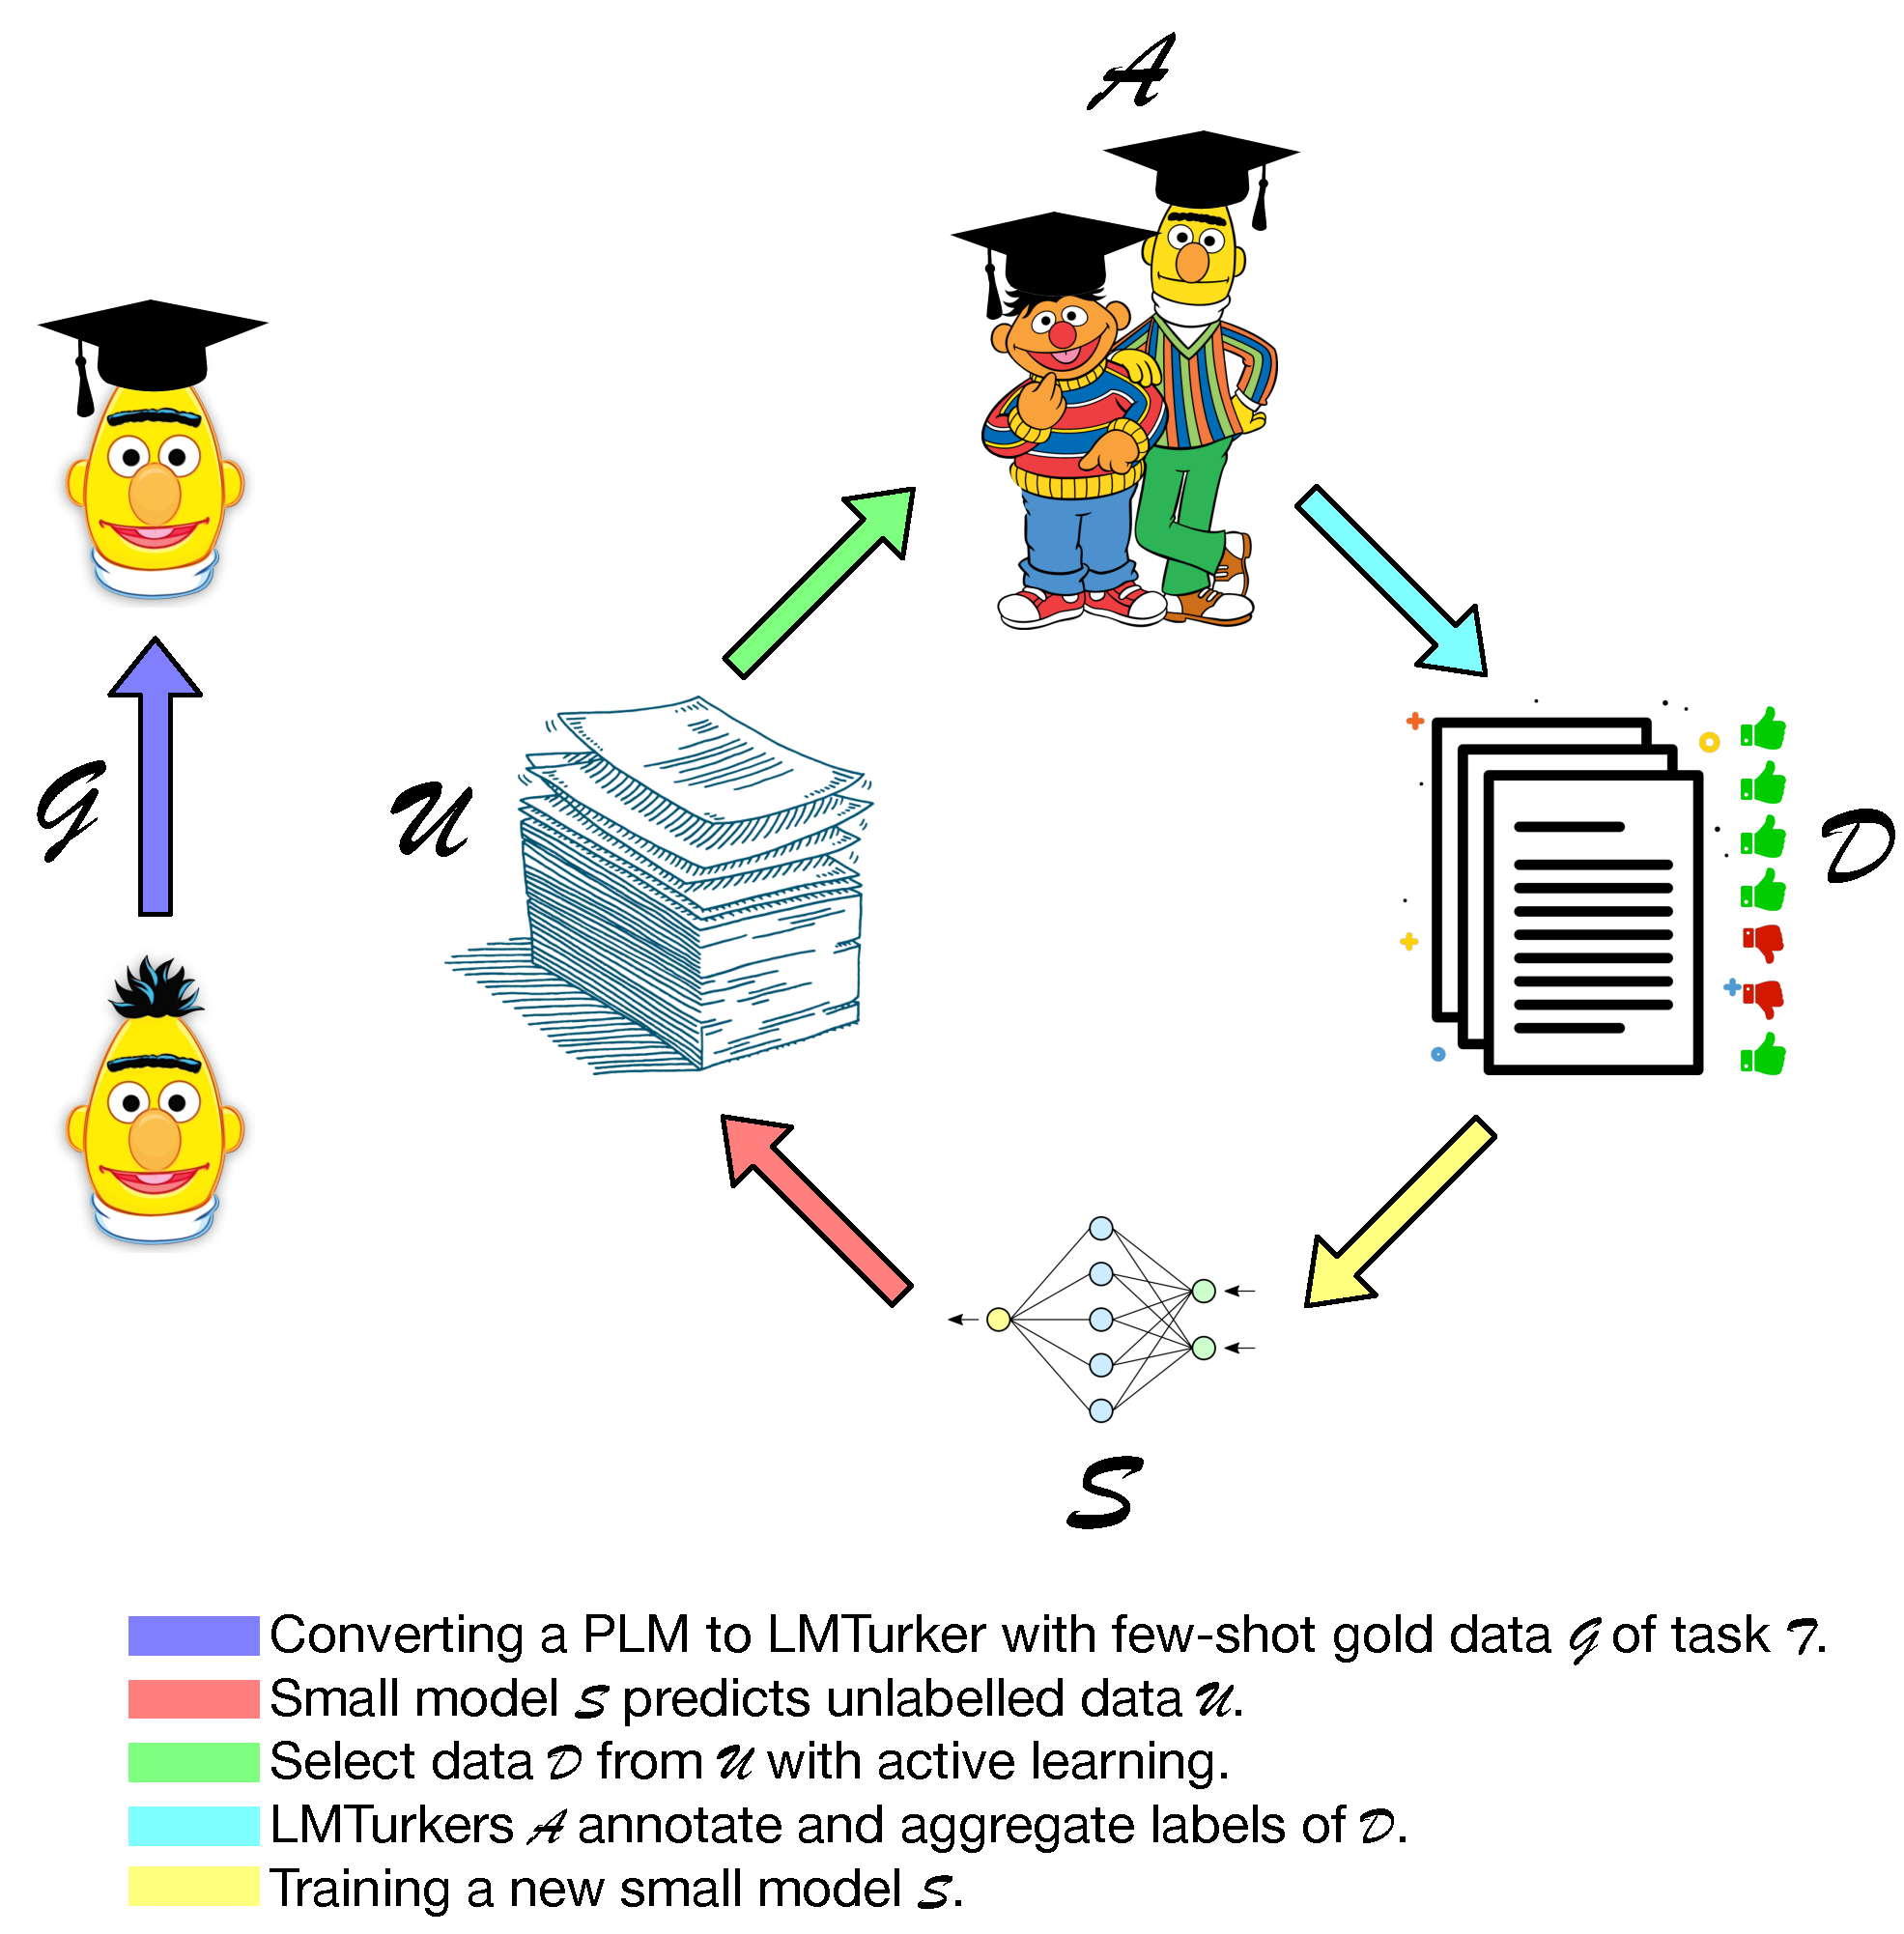
\includegraphics[width=\linewidth]{imgs/overallframework.pdf}
\caption{
  \md overview; best viewed in color.
  We few-shot adapt PLMs to task $\mathcal{T}$ (left) and
  then use them as crowdsourcing workers in active learning.
  We show that these PLM workers are effective in training a small model
{\cal $\mathcal{S}$} through a customized active learning loop (right).
\md is a novel way to take advantage of large-scale PLMs:
It creates models small enough to be deployed in resource-limited
real-world settings.}
\figlabel{overallframe}
\end{figure}


Our goal in this paper is to devise
methods that make
\emph{more effective use of
  current few-shot learners}.
This is crucial because
an increasing number of
gigantic few-shot learners are trained;
how to use them effectively is thus
an important question.
In particular,
we want an alternative to
hard-to-deploy huge models.
At the same time, we want to take full advantage of the PLMs'
strengths:
Their versatility
ensures 
wide applicability across tasks;
their vast store of knowledge
about language and the world
(learned in pretraining)
manifests in the
data efficiency of
few-shot learners, reducing
labor and time consumption
in data annotation.



In this work, we propose
\textbf{\md},
\textbf{L}anguage
\textbf{M}odel as
mechanical \textbf{Turk}.
Our basic idea (see \figref{overallframe}) is that, for an NLP task \tasksymbol,
\emph{we treat few-shot learners as non-expert workers},
resembling crowdsourcing workers that annotate resources for
human language technology.
We are inspired by the fact that  we can view a
crowdsourcing worker
as a type of few-shot learner:  A few examples
demonstrating $\mathcal{T}$ teach her
enough about $\mathcal{T}$ to
conduct effective annotation.
For example, \citet{snow-etal-2008-cheap} train workers
with a few examples of annotating emotion;
\citet{he-etal-2015-question} conduct short training sessions
for workers before annotation;
\citet{lee2021annotation}  train
workers with
learning curricula.

\citet{snow-etal-2008-cheap} pioneered crowdsourcing
in NLP \citep{howe2006rise,howe2008crowdsourcing}, motivated
by the high cost of TreeBank annotation \citep{marcus-etal-1993-building,
miller-etal-1993-semantic}.
Crowdsourcing organizes
human workers over the Web
to annotate data.
Workers need not be experts to be effective, resulting in
reduced \emph{per-label cost}.
Active learning \citep{hachey-etal-2005-investigating,felder2009active} can be incorporated
\citep{laws-etal-2011-activeb} to further decrease annotation cost, by lowering
\emph{the number of labels}
to be annotated.
\md treats PLM-based
few-shot learners as
non-expert workers that
produce training sets, which are
then used to
train a small
machine learning model
$\mathcal{S}$ specialized for
\tasksymbol.
This
scenario is analogous to
active learning.
We achieve two benefits:
(i) low annotation cost
because humans only need to annotate a few shots of data;
(ii) solving practical
NLP tasks with small models
that are more real-world deployable.


\md
resonates with
\citet{laws-etal-2011-activeb}'s
earlier idea of
combining crowdsourcing and
active learning.
They consider
human workers
as ``noisy annotators''
while we explore the utilization
of modern NLP few-shot learners
(built upon machine learning models)
as workers --
which have the advantage of
being free,
instantly interactive,
fast, responsive, and non-stopping.


Our \textbf{contributions}: (i) We propose \md, a method
that uses few-shot learners as crowdsourcing workers.
\figref{overallframe} shows the overview of \md.
(ii) We vary an array of important design
choices, identifying strengths and weaknesses of \md.
(iii) Unlike much work on active learning  in
a synthetic oracle setting,
we develop methods for handling the
varying quality
of annotation  that does not come from an oracle.
(iv) We extensively evaluate \md on five
datasets, showing that \md can guide a small model
$\mathcal{S}$ to progressively improve on \tasksymbol.
$\mathcal{S}$ can then be deployed in practical scenarios.
(v) This is the
first work
showing that few-shot learners
give rise to effective NLP models
through crowdsourcing and active
learning -- with the benefits of low annotation cost and
practical deployability.


\section{Related Work}
\textbf{Few-shot learners in NLP}.
Significant progress
has been made in
developing \citep{devlin-etal-2019-bert,ELMopaper,XLNetpaper,GPT3paper},
understanding \citep{liulinguistic,tenney2018what,
  belinkov-glass-2019-analysis,hewitt-liang-2019-designing,
  hewitt-manning-2019-structural,zhao-etal-2020-quantifying,
  BERTologypaper},
and utilizing \citep{
  adapterpaper,maskingpaper,
  GPT3paper,lisaprefix,
  PETpaper,Prompttuningpaper,mi2021cins}
PLMs.
\citet{GPT3paper},
\citet{PETpaper},
and \citet{Ptuningpaper}
show that PLMs can serve as
data-efficient few-shot learners,
through priming or prompting \citep{liu2021pre}.
For example, GPT3 achieves
near state-of-the-art
performance on COPA \citep{roemmele2011choice}
with only 32 annotated data.


However,
little to no
work discusses
or explores the
actual \emph{practical utility}
of these few-shot learners.
We aim to develop
effective methods of
utilizing them
in practical scenarios.



\textbf{Crowdsourcing} has a
long history
in human language technology
\citep{crowdsourcingagg,callison-burch-2009-fast,
  trautmann2020fine}; specialized
workshops were
organized
\citep{crowdsourws,emnlp-2019-aggregating}.
It has numerous applications
\citep{crowdsourcingsurvey},
but we focus on its
application as
voting systems.
To reduce \emph{per-label} cost,
crowdsourcing organizes
non-expert human workers
distributed across the Web for annotation,
instead of employing linguistic experts
\citep{jamison-gurevych-2015-noise,
  bhardwaj-etal-2019-carb,
  nangia-etal-2021-ingredients}.
\citet{snow-etal-2008-cheap}
show that
averaging ten crowdsourced labels
matches an expert-level label for
recognizing textual entailment \citep{rtedata}.
\citet{paun-etal-2018-comparing}
show that incorporating structure in
annotation models is important.
Measuring label disagreements
is also crucial \citep{dumitrache2021empirical}.



\md
utilizes NLP few-shot learners
as non-expert workers.
The few-shot training data
can be viewed as the examples
shown
to humans before annotating.
The process is
free, fast, responsive, and non-stopping.



\textbf{Active learning} (AL; \citet{cohn1996active,settles2009active})
strives to reduce \emph{the number of examples}
to be annotated
via identifying 
informative examples
with acquisition functions.
\citet{settles-craven-2008-analysis}
evaluate AL algorithms
for sequence labeling. 
\citet{ALCNN,shen-etal-2017-deep,siddhant-lipton-2018-deep}
apply  AL to deep neural networks.
\citet{simpson-gurevych-2018-finding} devise
a scalable Bayesian
preference learning method for
identifying convincing arguments.
\citet{lee-etal-2020-empowering} propose to consider
user feedback in AL systems.
\citet{ein-dor-etal-2020-active} explore AL
for BERT.
\citet{schroder2020survey} review
text classification with AL.
\citet{liang-etal-2020-alice,margatina2021active}
integrate contrastive learning into AL.
\citet{zhang-plank-2021-cartography-active} identify
examples with datamap \citep{datasetmap}.

We incorporate AL in
\md to
reduce the amount of examples
to be annotated by PLMs,
reducing the
computational cost
of running several
inference passes.
This contributes to a more
environmentally
friendly \citep{strubell-etal-2019-energy,
  schwartz2020green,patterson2021carbon} 
scenario.


Perhaps  closest to our work,
\citet{yoo2021gpt3mix}
conduct data augmentation
via priming GPT3 and
\citet{wang2021want} mix
human- and GPT3-annotated data, focusing
on cost analysis.
GPT3 is utilized in
a Language-Model-as-a-Service form by OpenAI,
which is not free.\footnote{\url{https://beta.openai.com/pricing}}
Also, strategies of priming GPT3 may not
generalize well to other PLMs.
For example, priming strategies have to adapt to GPT3's maximum
sequence length.  However, maximum sequence length -- as a
hyperparameter -- could vary across PLMs.
In this work,
we prompt
publicly available free PLMs.
This also makes the process more flexible; for example,
the PLM can be updated
with gradient descent.




\section{\md}
\subsection{Training few-shot learners}
We first adapt a PLM to
task $\mathcal{T}$ with
a few-shot human-labeled gold dataset
$\mathcal{G}$ = \{$\mathcal{G}_{train}; \mathcal{G}_{dev}$\}
of \tasksymbol.
This procedure mimics
one of the initial but crucial
steps in crowdsourcing:
A few example annotations
are shown to the workers,
demonstrating \tasksymbol; workers
learn about the task and then start
annotating \citep{
snow-etal-2008-cheap,
he-etal-2015-question,
roit-etal-2020-controlled,
trautmann2020fine,
lee2021annotation}.





We achieve this adaptation
through P-Tuning \citep{Ptuningpaper}.
Taking movie review classification
as an example,
the goal is to associate
a binary label $y$ from \{-1, +1\}
to an input sentence
$\mathbf{x} = (x_1, ..., x_n)$ where
$x_i$ refers to a token.
Unlike finetuning and
its variants \citep{devlin-etal-2019-bert,adapterpaper,maskingpaper}
that train a classifier head,
P-Tuning reformulates a sentence into a
cloze-style query;
the PLM is then requested to
respond to the query
with an answer selected from
a list of candidates.
Concretely, an input pair

\begin{itemize}
\item[] \small{($\mathbf{x}$, y) = (``watching it leaves you giddy.'', -1)}
\end{itemize}

\noindent is reformulated to:

\begin{itemize}
\item[] \small{``\underline{[v]} watching it leaves you giddy. \underline{It} \underline{is} [MASK] \underline{.}''}
\end{itemize}

\noindent in which the \underline{underlined} tokens are
prompting words that give the model
a hint about \tasksymbol.
``[v]'' -- whose trainable embedding vector is
randomly initialized -- is a
prompting token injecting extra free parameters.
The PLM is then requested to pick a word
from \{``bad'', ``good''\} to
fill in the position of ``[MASK]''.
A mapping
\{``bad''$\,\to\,$-1, ``good''$\,\to\,$+1\}
is used to
transform the selected answer
to a label such that standard evaluation
measures like accuracy can be computed.
Prompting has been shown to effectively
adapt a PLM to $\mathcal{T}$
\emph{with only a few annotations};
see \citep{liu2021pre} for a
comprehensive review of prompting.
We refer to a PLM adapted to $\mathcal{T}$ as
an \textbf{\mdr} $A$.


We select
prompting words and mappings based on the
small development set $\mathcal{G}_{dev}$.
\secref{promptingdetails} provides
details on prompting and datasets.

\subsection{Aggregating annotations}
\seclabel{subsec:aggregateannotations}
Individual workers are subject to annotation biases
\citep{snow-etal-2008-cheap};
therefore, crowdsourcing often collects labels from
several workers \citep{crowdsourcingsurvey}
for an
example $\mathbf{x}$ and then
aggregates them
for quality control
\citep{crowdsourcingagg}.
It is straightforward to obtain
a group of \mdrs
$\mathcal{A}=\{A_1, ..., A_k\}$,
by adapting the PLM to $\mathcal{T}$
with $k$ different prompts.
A querying sentence $\mathbf{x}$
is then annotated by every \mdr,
resulting in a list of labels
$\mathbf{y} = [y_1, ..., y_k]$.
We evaluate different methods
aggregating $\mathbf{y}$ to a single
label $\hat{y}$.


\textbf{BestWorker}.
Among the $k$ \mdrs,
we pick the one
performing best on the dev set $\mathcal{G}_{dev}$.



\textbf{MajorityVoting}.
We select the
most frequent
label in
$\mathbf{y} = [y_1, ..., y_k]$
as $\hat{y}$.


To estimate
an \mdr's confidence on label $y_i$,
we compare the
logits\footnote{
  Calibration can be conducted to
  further improve the estimation
  \citep{guo2017calibration}.
  We leave this to future work.
} computed by the  PLM:
$${\scriptstyle y_i \ =\  \argmax(\text{logit}(y^1),...,\ \text{logit}(y^N)) ,}$$
\noindent where
$N$ refers to the label set size,
e.g., $N$=2 for $y$ from \{-1, +1\}.
We then can evaluate several methods of
aggregating annotations according to 
PLM logits.

\textbf{LogitVoting}.
We average the logits from all  $k$ \mdrs
$\{A_1, ..., A_k\}$
to compute $\hat{y}$:
$${\scriptstyle \hat{y}\ =\ \argmax(\frac{1}{k}\sum_{i=1}^k\text{logit}(y^1_i),...,\frac{1}{k}\sum_{i=1}^k\text{logit}(y^N_i))}.$$


\textbf{WeightedLogitVoting}.
We use \mdrs' performance on $\mathcal{G}_{dev}$ 
to weight their logits and then aggregate the
predictions:
%\small
%$$\hat{y}=\argmax(\sum_{i=1}^kw_i\mbox{logit}(y^1_i),...,\sum_{i=1}^kw_i\mbox{logit}(y^N_i)) ,$$
%$$w_i = f(A_i, \mathcal{G}_{dev}) / \sum_{i=1}^k f(A_i, \mathcal{G}_{dev}) ,$$ 
%\normalsize
\begin{eqnarray*}
&{\scriptstyle \hat{y}\ =\ \argmax(\sum_{i=1}^kw_i\text{logit}(y^1_i),...,\sum_{i=1}^kw_i\text{logit}(y^N_i))} \\
&{\scriptstyle w_i\ =\ f(A_i, \mathcal{G}_{dev}) / \sum_{i=1}^k f(A_i, \mathcal{G}_{dev})}  
\end{eqnarray*}


\noindent where $f(A_i, \mathcal{G}_{dev})$ is the
performance of the 
$i$th \mdr $A_i$ on $\mathcal{G}_{dev}$.


We collect and aggregate annotations
from five \mdrs, 
i.e., we use $k$=5 in our experiments.



\subsection{Training a small model $\mathcal{S}$}
\seclabel{methodtrainingsmall}
After adapting \mdrs to $\mathcal{T}$
through prompting with the
few-shot gold dataset $\mathcal{G}$,
we next train a small model
$\mathcal{S}$
specialized to solve \tasksymbol.
Though large PLMs
are versatile and strong performers,
training and inference 
are faster and more
efficient for small models: They are more
deployable in resource-restricted
scenarios, e.g., on
edge devices \citep{jiao-etal-2020-tinybert}.

We mimic
pool-based active learning (AL; \citet{settles2009active})
to train $\mathcal{S}$.
The motivation is to
avoid frequent 
querying of \mdrs
$\mathcal{A}$ because
energy and time consumption
of PLM inference  is
costly
when
the number of queries
and $|\mathcal{A}|$ are large.

Concretely, pool-based AL
assumes a large
collection of unlabeled data
$\mathcal{U}$ = \{$\mathbf{x}_1,...,\mathbf{x}_M$\}
for \tasksymbol.
$\mathcal{S}$ is first trained with
$\mathcal{G}$ = \{$\mathcal{G}_{train}; \mathcal{G}_{dev}$\}.
After that,  a group of examples
$\mathcal{B}$ from $\mathcal{U}$ is sampled (c.f. \secref{alacquisition}),
which \mdrs  annotate.
Next, the annotated and aggregated examples 
$\mathcal{B'}$ are concatenated with
$\mathcal{G}$ to train $\mathcal{S}$.
The procedure is repeated iteratively,
such that the training data for
$\mathcal{S}$ keeps expanding.
We denote as $\mathcal{S}^j$ the model trained after
the $j$th iteration.
Note that $\mathcal{S}$ is trained from
scratch in each iteration \citep{cohn1994improving}.

\subsubsection{AL acquisition function}
\seclabel{alacquisition}
At the beginning of the $j$th iteration, 
a straightforward strategy
of sampling $\mathcal{B}$ from $\mathcal{U}$
is \textbf{random sampling}.
AL promises to select
a more informative $\mathcal{B}$
such that the trained
$\mathcal{S}^j$ performs better,
under the same budget.
These strategies -- or
\emph{acquisition functions} -- 
rely on $\mathcal{S}^{j-1}$,
i.e.,
$\mathcal{S}$
from the previous iteration:
$\mathcal{S}^{j-1}$ is employed to infer
$\mathcal{U}$
to obtain labels and logits
$\mathcal{P}^{j-1} = \{(y_1,\mathbf{c}_1),...,(y_M,\mathbf{c}_M)\}$;
each $\mathbf{c}_i$ contains
the logits of the  $N$ labels;
$y_i=\argmax(\mathbf{c}_i)$.
We explore
two common
AL acquisition functions:
Entropy \citep{roy2001toward}
and
LeastConfident \citep{lewis1994sequential}.



\textbf{Entropy} selects
from $\mathcal{P}^{j-1}$
examples with the
largest prediction entropy,
computed using $\mathbf{c}$.
Large entropy of an example $\mathbf{x}$
implies that $\mathcal{S}^{j-1}$
is unsure about which label to select;
$\mathbf{x}$ is then a query made to \mdrs
to obtain its label $\hat{y}$.
$(\mathbf{x}, \hat{y})$ is subsequently
added to $\mathcal{G}_{train}$ for training $\mathcal{S}^{j}$.


\textbf{LeastConfident}
selects from $\mathcal{P}^{j-1}$
examples for which the maximum
logit in $\mathbf{c}$ is the smallest.
Selected examples are then annotated 
and added to $\mathcal{G}_{train}$
for training $\mathcal{S}^{j}$.

Our AL setup is fairly standard, both in terms of
acquisition functions
and iterative enlargement by new
sampled data $\mathcal{B}$ at iteration
$j$ labeled by $\mathcal{S}^{j-1}$.


\subsubsection{Considering annotation quality}
\seclabel{instancetresholdingintro}
As in any realistic AL scenario, annotations are not perfect:
\mdrs
do not score perfectly on \tasksymbol.
As a result,
\emph{annotation quality of \mdrs
needs to be taken into consideration
before training} $\mathcal{S}^{j}$.
Denoting the training data of
$\mathcal{S}^{j}$ as $\mathcal{D}^{j}$,
we explore
a strategy of processing
$\mathcal{D}^{j}$, based on 
\mdr logits $\mathbf{l}$.


\textbf{InstanceTresholding}.
We preserve examples
$(\mathbf{x}, \hat{y}, \mathbf{l}) \in \mathcal{D}^{j}$
for which entropy computed on
$\mathbf{l}$
is smallest.
$\mathcal{G}^{train}$ is always preserved because it
is human-labeled gold data.
Note that this is
different from the strategy of
sampling $\mathcal{B}$, where
we select from
$\mathcal{P}^{j-1}$
examples to which $\mathcal{S}^{j-1}$
is most unsure (computed with $\mathbf{c}$).
We evaluate\footnote{
Motivated by \citet{wang-etal-2017-instance},
we also investigate the effectiveness of
weighting training examples. However,
we do not observe noticeable improvements of
task performance. We list more details  in
Appendix \secref{appendix:instanceweighting}.}
the effectiveness
of processing $\mathcal{D}^j$
before training $\mathcal{S}^j$
in \secref{poolfilter}.









\subsection{Summary of \md}
\md can be viewed as
intermediate  between
self training \citep{yarowsky-1995-unsupervised,abney-2004-understanding,lee2013pseudo,mi2021self}
and AL.
Unlike self training, \md employs
\emph{external} models provide labels to
$\mathcal{S}$.
Different from the artificial setup used in many AL
experiments, the provided labels
\emph{do not have oracle quality};
so $\mathcal{S}$
must use the annotations more carefully.
We next conduct experiments
investigating the effectiveness of \md.



\section{Datasets and Setup}
\subsection{Dataset}
We evaluate \md on five datasets:
Binary (SST2) and
fine-grained (five classes)
sentiment classification (SST5)
with the Stanford Sentiment TreeBank
\citep{socher-etal-2013-recursive};
news article topic classification with the
AG's News Corpus (AGNews; \citet{agdataset});
recognizing textual entailment (RTE; \citet{rtedata});
assessing linguistic acceptability
(CoLA; \citet{warstadt-etal-2019-neural}).
Appendix \secref{appendix:checklist} reports
dataset statistics.
SST2/SST5 and AGNews are widely used
in crowdsourcing and AL \citep{
  laws-etal-2011-activeb,
  ein-dor-etal-2020-active,
  margatina2021active,
  zhang-plank-2021-cartography-active}.
RTE and CoLA
assess
the models' ability to understand
textual entailment
and linguistic phenomena -- as opposed to
text categorization.
We report Matthew’s correlation coefficient
for CoLA and accuracy for the others \citep{wang-etal-2018-glue}.


\textbf{Few-shot datasets}.
Recall \md uses a small
human-annotated dataset
$\mathcal{G} = \{\mathcal{G}_{train}; \mathcal{G}_{dev}\}$.
Denoting $n$ as the number of shots \emph{per class},
we sample $\mathcal{G}^n_{train}$ and $\mathcal{G}^n_{dev}$
for each of $n \in \{8, 16, 32\}$.
For SST2, RTE, and CoLA, we use the train and dev
sets of  GLUE \citep{wang-etal-2018-glue};
$\mathcal{G}^n_{train}$ and $\mathcal{G}^n_{dev}$ are
sampled from the train set;
the dev set is used as the test set.
For SST5 and AGNews, we use
the official datasets;
$\mathcal{G}^n_{train}$ 
($\mathcal{G}^n_{dev}$) is sampled from the
train (dev) set;
we report  performance on the test set.
We repeat the sampling process
with three random seeds.




\subsection{Training setup}
\seclabel{promptingdetails}
\citet{GPT3paper} show that
large model size is necessary
for strong few-shot performance.
We use ALBERT-XXLarge-v2
\citep{albert} -- of size 223M parameters --
as our large PLM, which is
adapted to be an \mdr $A$ of
$\mathcal{T}$ with $\mathcal{G}$.
With parameter reuse, ALBERT-XXLarge-v2 
outperforms
larger models
like the 334M
BERT-large \citep{devlin-etal-2019-bert}.
In contrast,
$\mathcal{S}$
must be small
to be deployable
in practical scenarios.
We use TinyBERT-General-4L-312D
\citep{jiao-etal-2020-tinybert},
which has 14.5M parameters.



We train -- with prompting --
the large PLM with $\mathcal{G}$
for 100 batch steps using  batch size 16,
AdamW \citep{adamw} and 
learning rate
5e-4 with linear decay.
We prompt the large PLM five times
to obtain five \mdrs;
Appendix \secref{appendix:promptingdetails}
shows
prompting details.
At each iteration,
we finetune  $\mathcal{S}$
for 20 epochs using  batch size 32,
Adam \citep{adampaper} and 
learning rate
5e-5.
Each experiment is run
with three different random seeds.
We use PyTorch \citep{torch} and  HuggingFace
\citep{wolf-etal-2020-transformers}.



\begin{table}[t!]
\scriptsize\centering\renewcommand{\arraystretch}{1.3}\setlength{\tabcolsep}{3pt}
\begin{tabular}{c|c|c|c}
      &\citet{PETpaper,schick2020s} & \citet{gao-etal-2021-making}   & Ours        \\ \hline
SST2  &n/a                          & 93.0$\pm$0.6    &         93.08$\pm$0.62  \\
SST5  &n/a                          & 49.5$\pm$1.7    &         46.70$\pm$0.93 \\
RTE   &69.8                         & 71.1$\pm$5.3    &         70.88$\pm$1.70  \\
AGN.  &86.3$\pm$0.0                 &  n/a            &         87.71$\pm$0.07 \\
CoLA  &n/a                          & 21.8$\pm$15.9   &         19.71$\pm$1.89  \\
\end{tabular}
\caption{
  \mdrs achieve comparable few-shot performance with the
  literature. We refer to \emph{PET} results in
  \citet{PETpaper,schick2020s} and results
  of \emph{Prompt-based FT (auto) + demonstrations} 
  in \citet{gao-etal-2021-making}.
}
\tablabel{fewshotperfcomp}
\end{table}

%%% Local Variables:
%%% mode: latex
%%% TeX-master: "acl_latex"
%%% End:
 


\begin{figure}[t]
  \centering
	\subfloat{
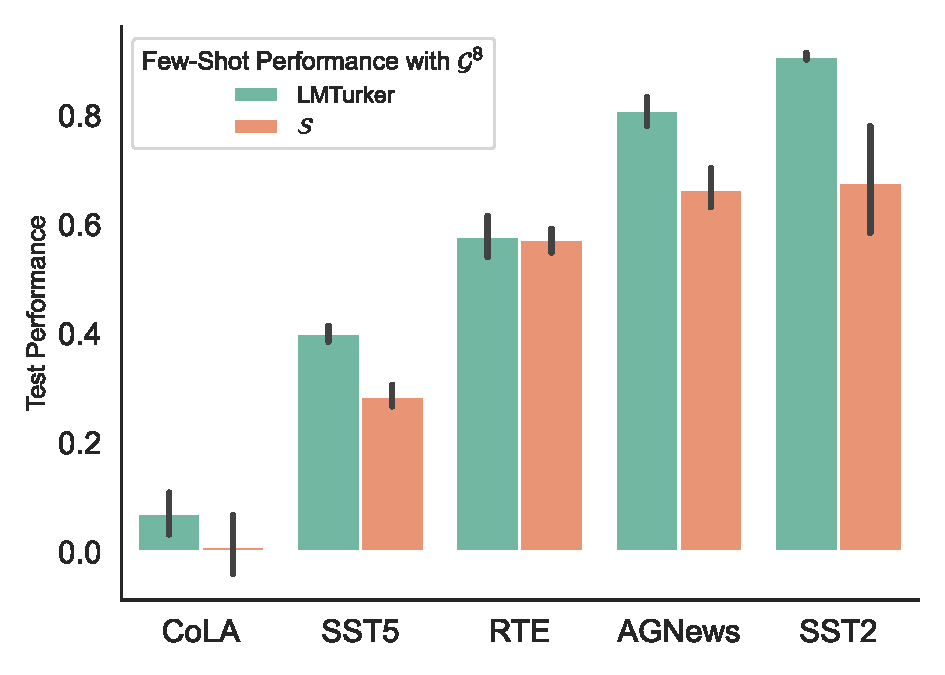
\includegraphics[width=.8\linewidth,height=0.25\textwidth]{imgs/init,perf,8.pdf}
      }\\
      \subfloat{
 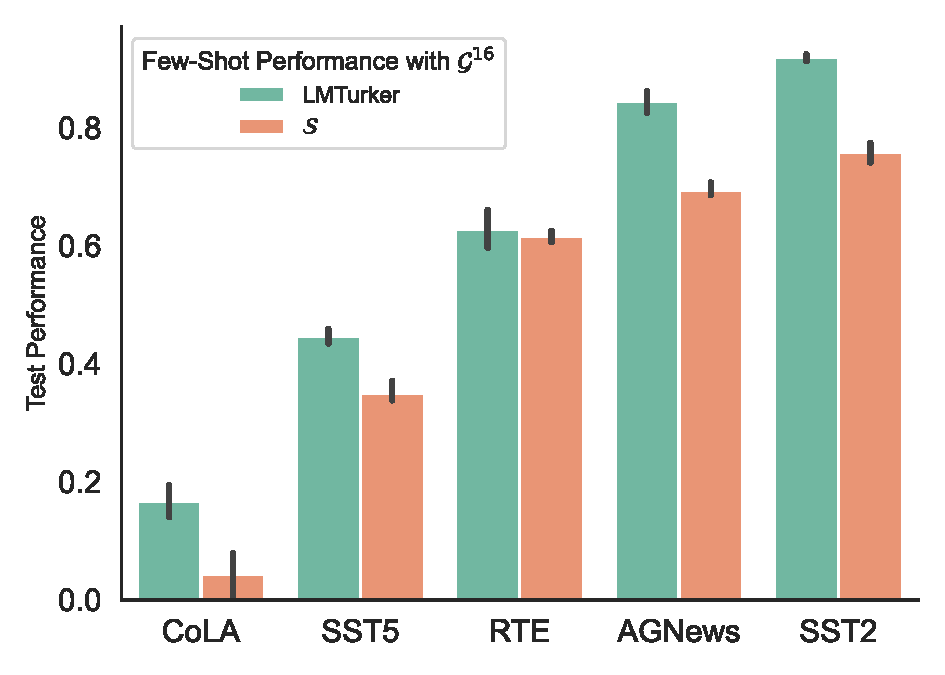
\includegraphics[width=.8\linewidth,height=0.25\textwidth]{imgs/init,perf,16.pdf}
       }
       \\
       \subfloat{
 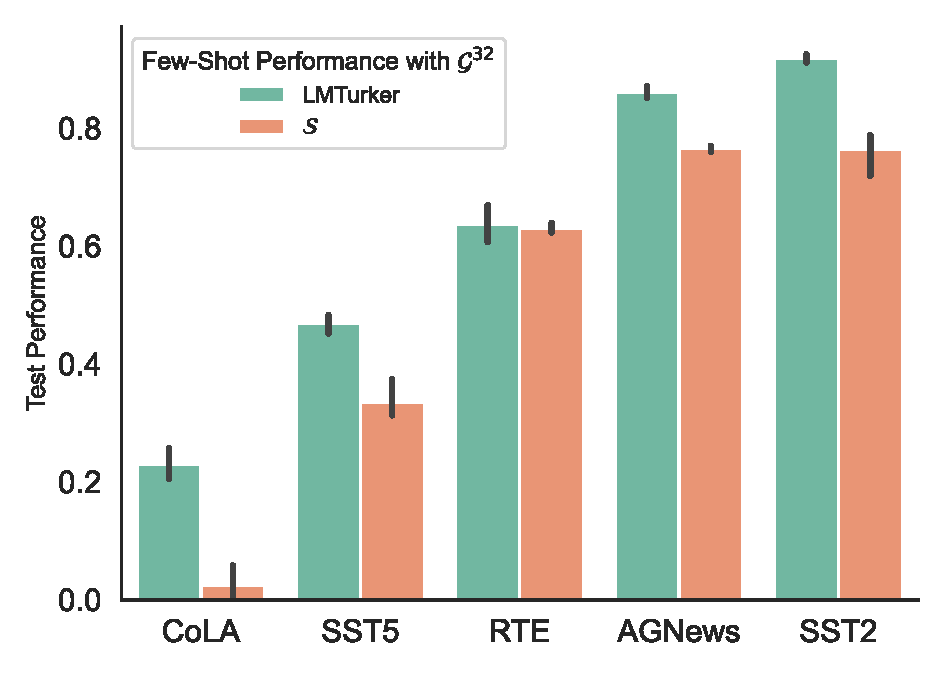
\includegraphics[width=.8\linewidth,height=0.25\textwidth]{imgs/init,perf,32.pdf}
 	}
\caption{
\emph{Few-shot} test set performance of
\mdrs and $\mathcal{S}$.
We use the few-shot gold datasets
$\mathcal{G}^8$ (top),
$\mathcal{G}^{16}$ (middle),
and $\mathcal{G}^{32}$ (bottom).}
\figlabel{fewshotperf}
\end{figure}


\section{Experiment}
\subsection{Few-shot performance (non-iterative)}
We compare few-shot performance
of \mdrs
and
the small model $\mathcal{S}$
when \emph{only $\mathcal{G}$ is used}.
\mdr performance
is comparable to prior work
\citep{PETpaper,schick2020s,gao-etal-2021-making}
as shown in \tabref{fewshotperfcomp}.


\figref{fewshotperf}
compares performance of \mdrs
and $\mathcal{S}$.
Appendix \secref{appendix:numeric}
\tabref{appendix:fewshotnumeric}
reports numeric values.
\mdrs perform clearly
better than $\mathcal{S}$
on CoLA, SST5, AGNews, and SST2; e.g.,
for SST2, for train/dev size 16,
\mdr
accuracy is 93.08\% vs.\ 75.83\% for
$\mathcal{S}$.
\mdrs' superiority
over $\mathcal{S}$  
on RTE is
modest.
As an inference task, RTE is more challenging than
classification (e.g., AGNews).
We hypothesize that current few-shot learners
require more data than $\mathcal{G}^{32}$ to
process difficult
tasks  better than
$\mathcal{S}$.  
Scaling up to even larger
PLMs is also a promising
direction \citep{GPT3paper,Prompttuningpaper}.


Overall,
\mdrs
outperform $\mathcal{S}$  
with clear margins,
evidencing that their annotations
can serve as supervisions for training
$\mathcal{S}$.
We next conduct iterative training
to improve performance of
$\mathcal{S}$ on $\mathcal{T}$
with supervisions from \mdrs.


\begin{figure}[h!]
\centering
\hspace{-.2cm}\vspace{-.25cm}\subfloat{
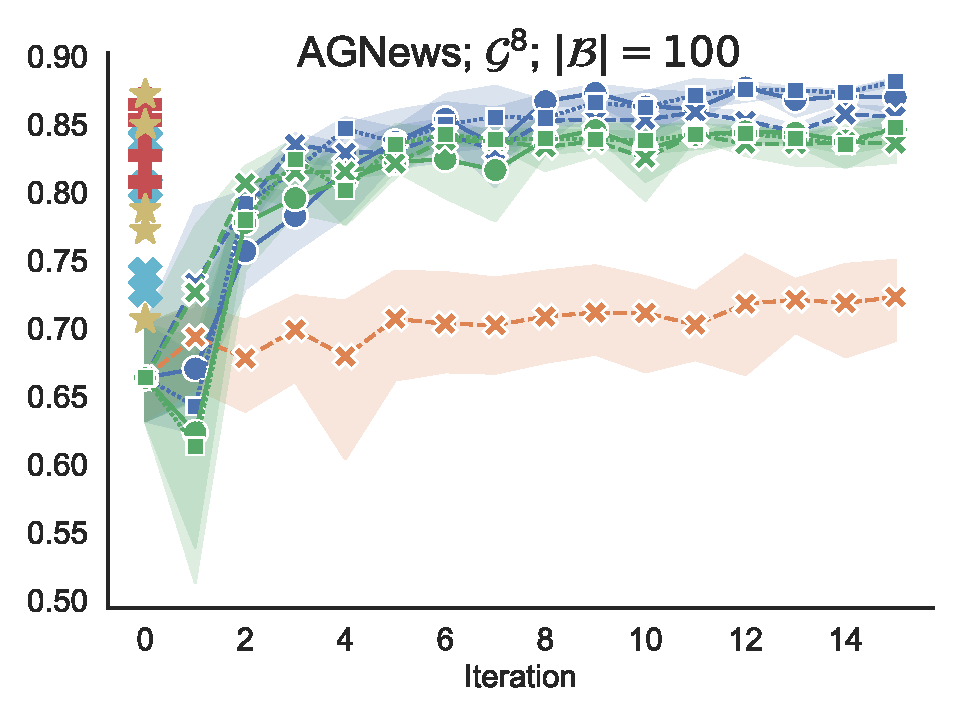
\includegraphics[width=.5\linewidth,height=0.2\textwidth]{imgs/_ag,MV,8,100.pdf}
}
\hspace{-.2cm}\vspace{-.25cm}\subfloat{
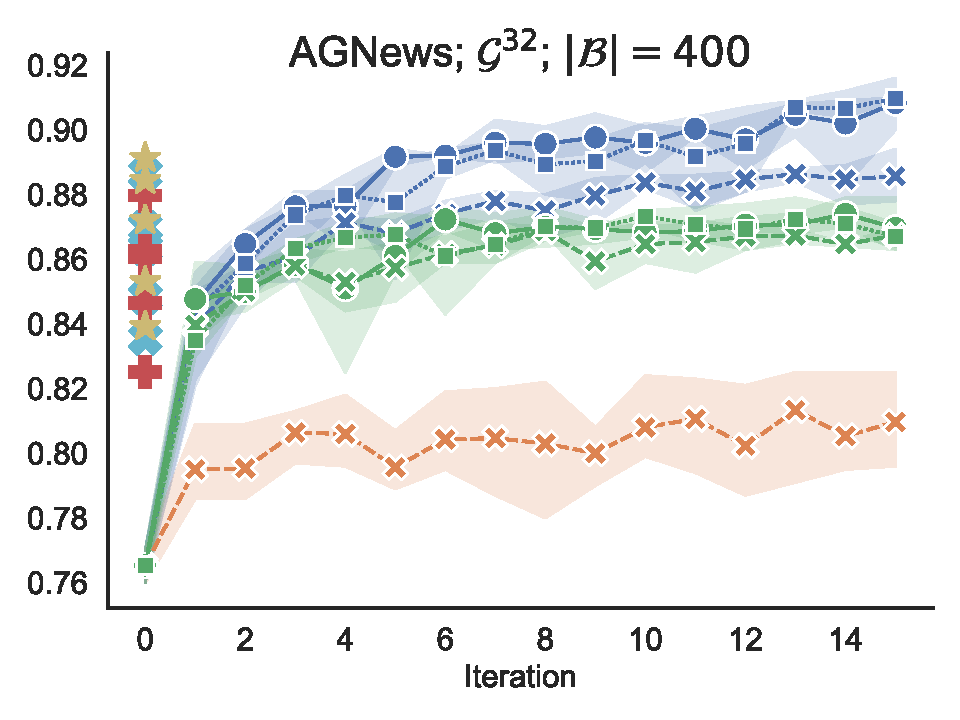
\includegraphics[width=.5\linewidth,height=0.2\textwidth]{imgs/_ag,MV,32,400.pdf}
}
\\
\hspace{-.2cm}\vspace{-.25cm}\subfloat{
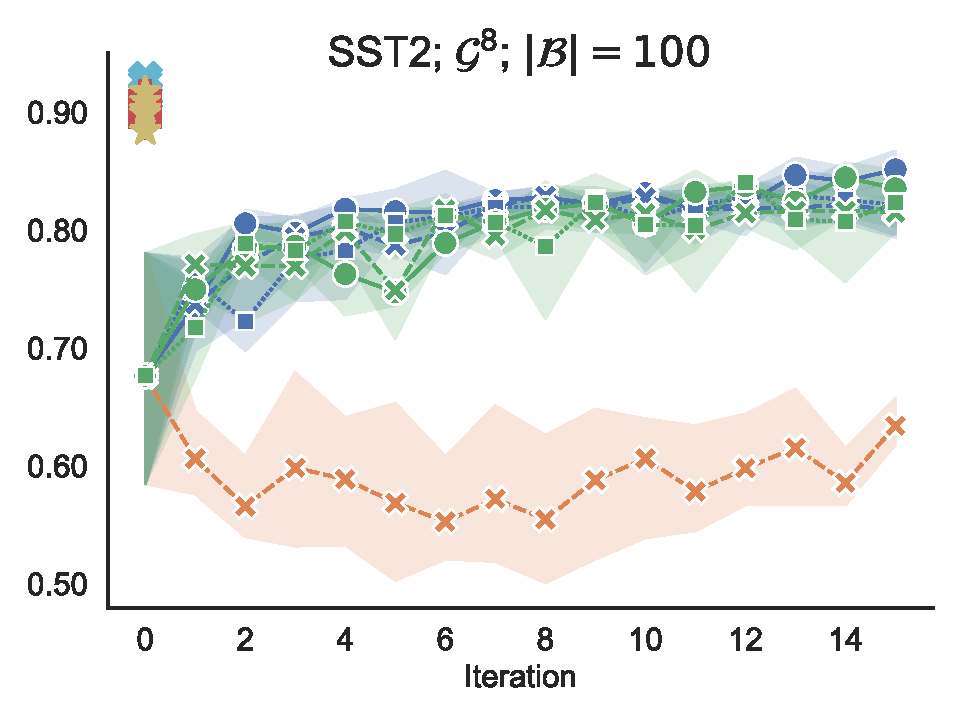
\includegraphics[width=.5\linewidth,height=0.2\textwidth]{imgs/_sst2,MV,8,100.pdf}
}
\hspace{-.2cm}\vspace{-.25cm}\subfloat{
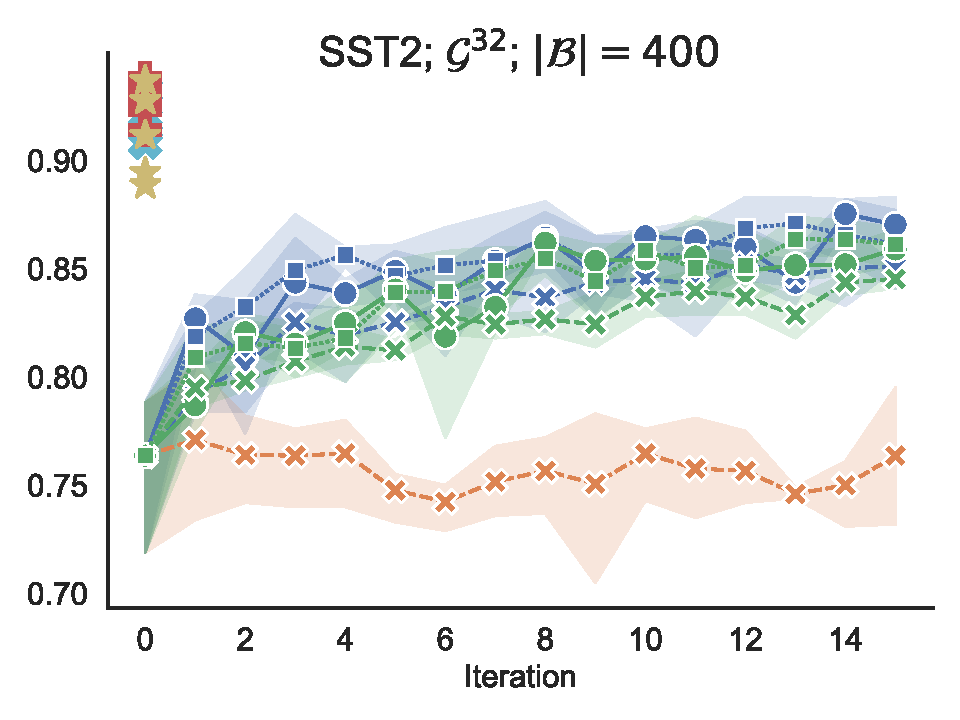
\includegraphics[width=.5\linewidth,height=0.2\textwidth]{imgs/_sst2,MV,32,400.pdf}
}
\\
\hspace{-.2cm}\vspace{-.25cm}\subfloat{
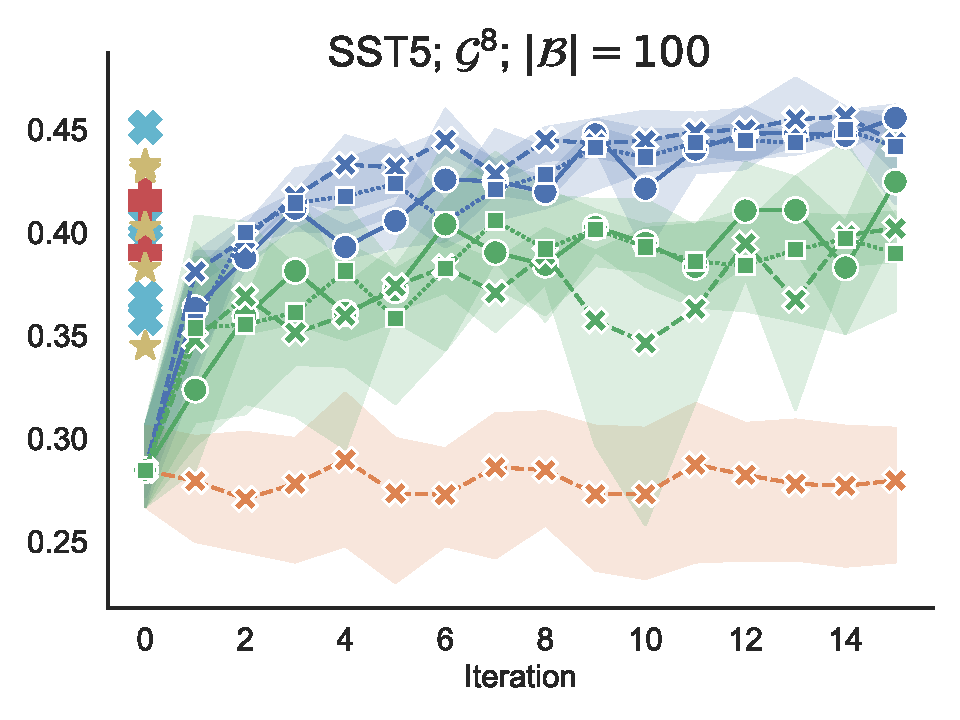
\includegraphics[width=.5\linewidth,height=0.2\textwidth]{imgs/_sst5,MV,8,100.pdf}
}
\hspace{-.2cm}\vspace{-.25cm}\subfloat{
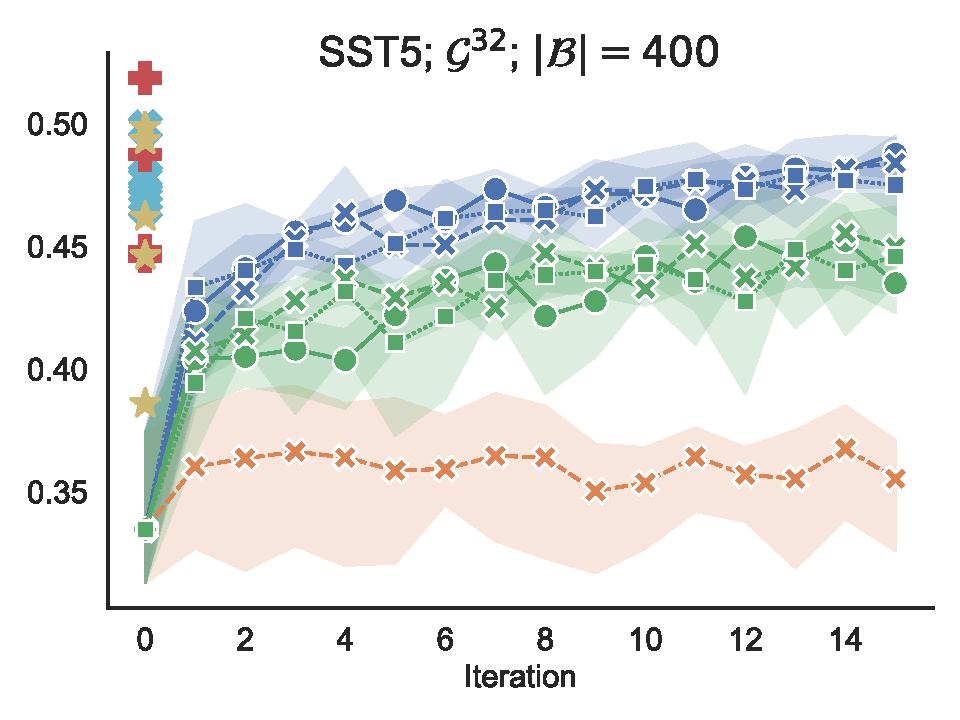
\includegraphics[width=.5\linewidth,height=0.2\textwidth]{imgs/_sst5,MV,32,400.pdf}
}
\\
\hspace{-.2cm}\vspace{-.25cm}\subfloat{
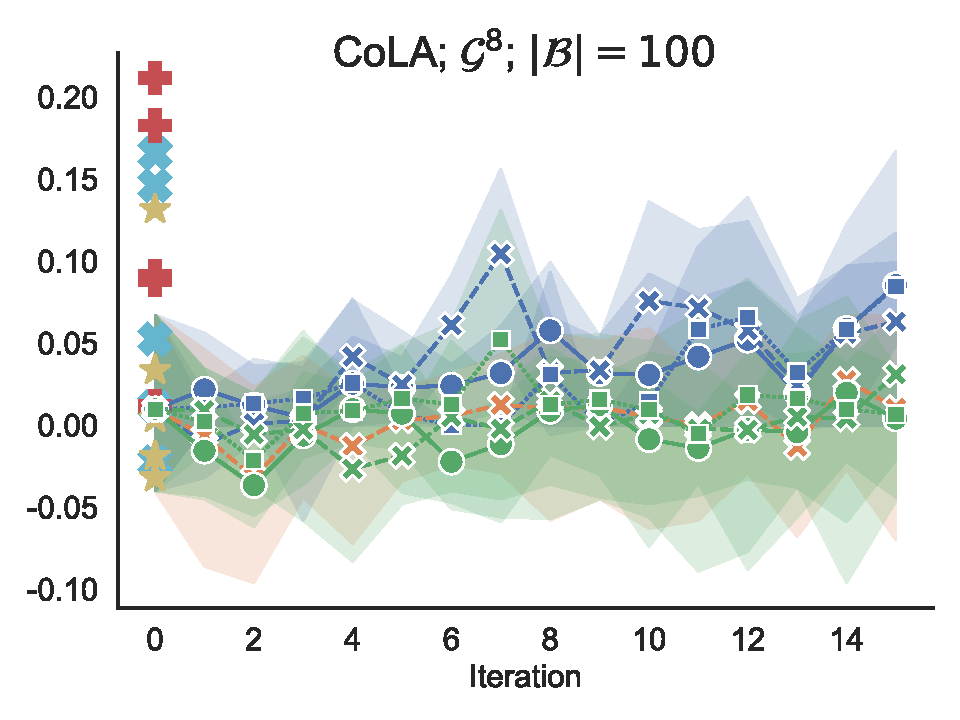
\includegraphics[width=.5\linewidth,height=0.2\textwidth]{imgs/_cola,MV,8,100.pdf}
}
\hspace{-.2cm}\vspace{-.25cm}\subfloat{
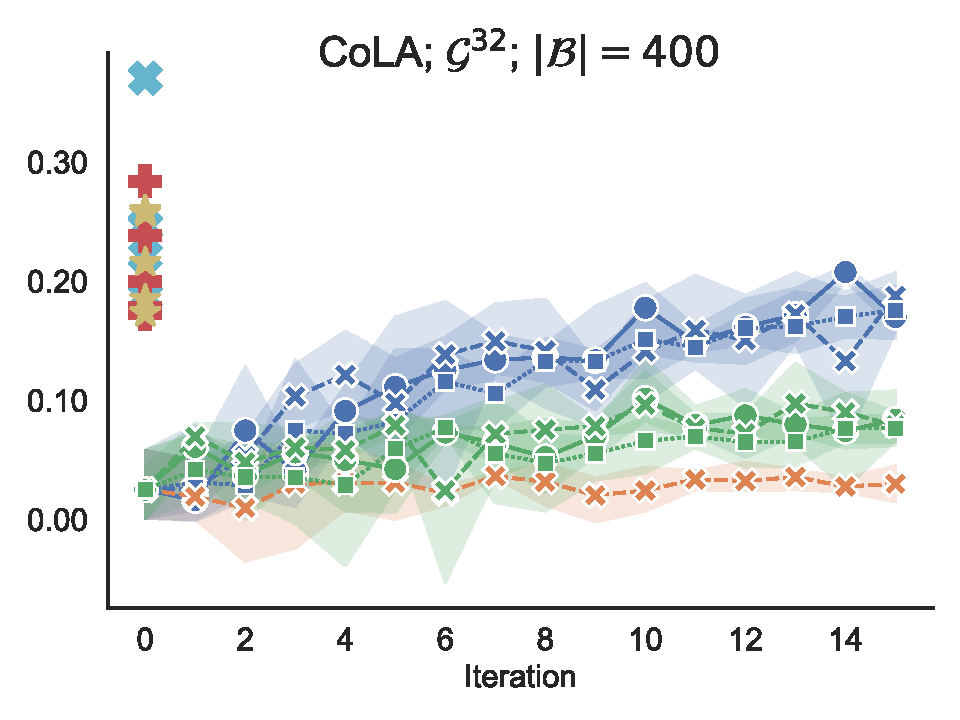
\includegraphics[width=.5\linewidth,height=0.2\textwidth]{imgs/_cola,MV,32,400.pdf}
}
\\
\hspace{-.2cm}\vspace{-.2cm}\subfloat{
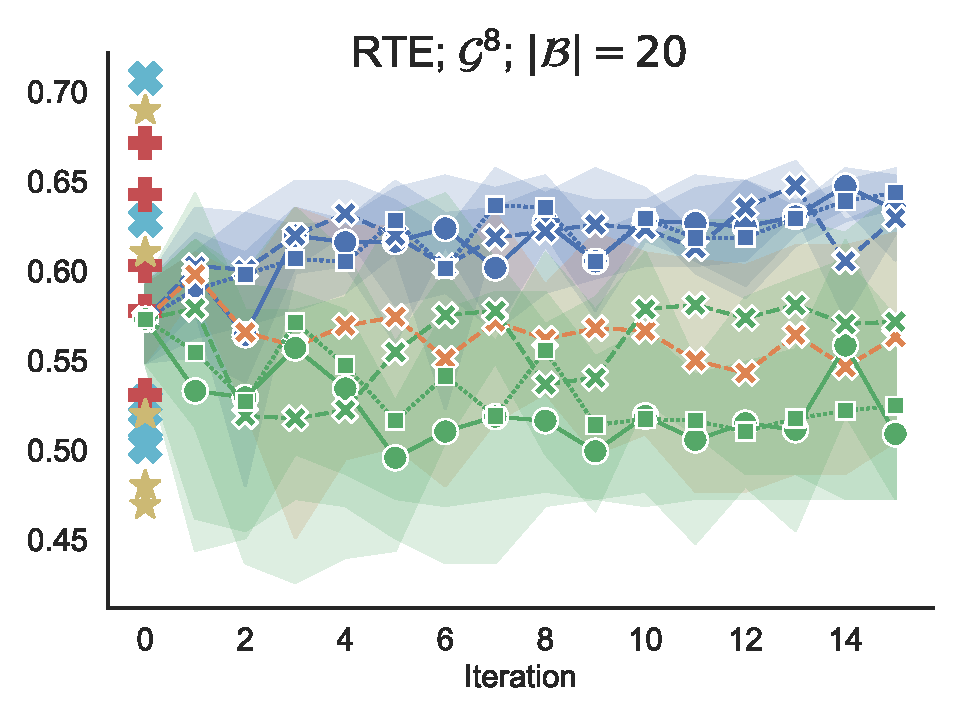
\includegraphics[width=.5\linewidth,height=0.2\textwidth]{imgs/_rte,MV,8,20.pdf}
}
\hspace{-.2cm}\vspace{-.2cm}\subfloat{
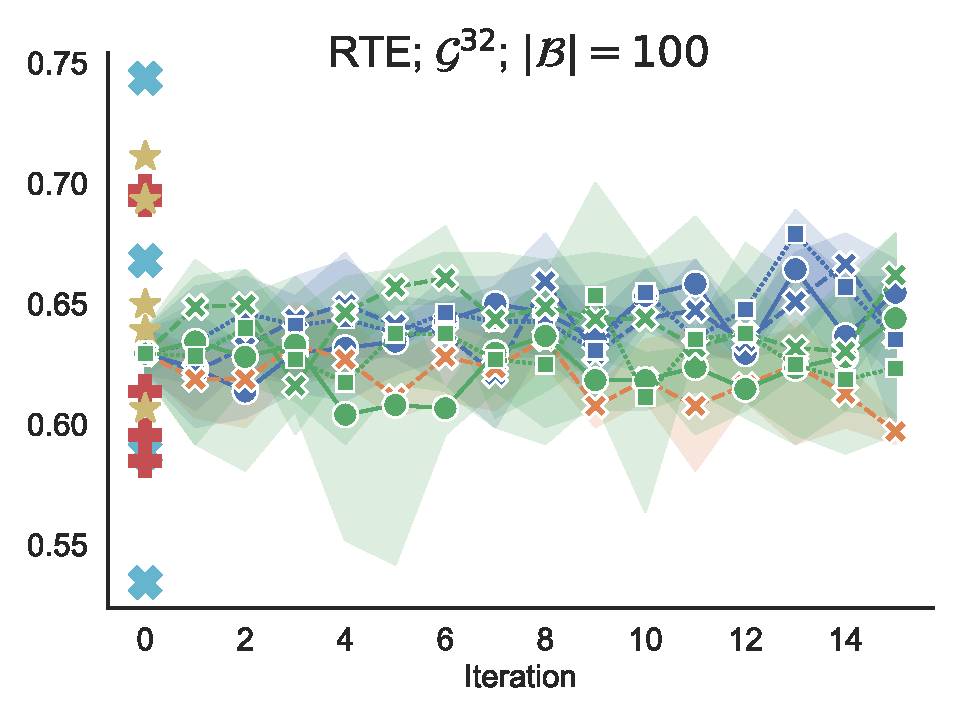
\includegraphics[width=.5\linewidth,height=0.2\textwidth]{imgs/_rte,MV,32,100.pdf}
}
\caption{
  Improving $\mathcal{S}$ with
  \textcolor{blue}{active learning (blue)},
  \textcolor{orange}{self training (orange)},
  and
  \textcolor{green}{\md (green)}.
  Free markers at step zero show \mdr performances;
  colors distinguish random seeds.
  Three acquisition functions are:
  Entropy ($\bullet$),
  LeastConfident (\tiny$\blacksquare$\normalsize),
  random sampling (\tiny\XSolidBold\normalsize).
  At iteration $j$, each experiment is repeated
  three times; we show
  mean and standard deviation.
  Appendix \figref{appendix:completeiteratives}
  visualizes more results.
}
\figlabel{iterative}
\end{figure}



\subsection{Iterative training}
We investigate
the effectiveness
of \md
by simulating
scenarios
analogous to
active learning.
Concretely,
we compare three
schemes of annotating
the sampled data
$\mathcal{B}$
at each annotation iteration $j$:

\begin{itemize}
\item \textcolor{blue}{Active learning (AL)}. We use $\mathcal{B}$'s
  \emph{gold labels} to show how $\mathcal{S}$ performs with expert
  annotations.  Gold labels are ideal, but costly because expert
  annotators need to be employed.

\item   \textcolor{orange}{Self training (ST)}.
  We use $\mathcal{S}^{j-1}$,
  the  model trained in
  the previous iteration,
  to annotate
  $\mathcal{B}$ \citep{yarowsky-1995-unsupervised,abney-2004-understanding,lee2013pseudo}.
  ST trades supervision
  quality for
  annotation cost;
  no extra cost is introduced.
  Because there is
  no external
  supervision,
  ST is expected to be a baseline.

\item   \textcolor{green}{\md}.
  We query the \mdrs
  to annotate $\mathcal{B}$.
  \mdrs
  are machine learning models, so there is no human labor.
  Based on
  the findings in \figref{fewshotperf}, \mdr supervisions
  are expected to have better quality
  than those of ST.
  Yet \md could fall behind
  AL because \mdr labels are not gold labels.
\end{itemize}


When sampling
$\mathcal{B}$ from $\mathcal{U}$ at
each iteration $j$,
we consider the strategies
described in
\secref{methodtrainingsmall}.
We employ Random for all three schemes and
Entropy/LeastConfident for
AL/\md.
Entropy and LeastConfident 
rely on $\mathcal{S}^{j-1}$.
Regarding the number of sampled examples,
we experiment with
$|\mathcal{B}|$=100 and $|\mathcal{B}|$=400
for SST2, SST5, AGNews,  CoLA.
Due to RTE's small size, we use
$|\mathcal{B}|$=20 and $|\mathcal{B}|$=100.
We run for 15 iterations of improving $\mathcal{S}$.
To aggregate annotations from \mdrs,
we use MajorityVoting
(\secref{subsec:aggregateannotations}),
which is widely used in crowdsourcing.
See \secref{varyaggregations} for a comparison
of various  aggregation methods.

\figref{iterative}
\textbf{compares AL, ST, and \md.}
ST (orange)
noticeably helps $\mathcal{S}$ to perform
progressively better on AGNews, e.g., when
comparing
$\mathcal{S}^{15}$ to $\mathcal{S}^{0}$
shown in
the first row, especially when $|\mathcal{B}|$=400.
However, we do not
identify clear
improvements
when looking at other tasks.
Except for RTE-$\mathcal{G}^{8}$,
ST clearly falls behind AL and \md.
This inferior performance
meets our expectation because
there is no
external supervision assisting
$\mathcal{S}$ to perform better
on \tasksymbol.
In what follows,
we omit ST for
clearer visualization and discussion.

AL (blue) performs
the best in most experiments.
However, this comes with extra
costs that are
not negligible: \emph{At each iteration},
human annotators need to
annotate 100--400 sentences.


\md (green) holds
a position
between AL and ST
on AGNews, SST2, SST5, and CoLA.
Somehow surprisingly,
\md performs almost comparably
to AL on SST2.
Unlike AL, \md
requires very little human labor;
the only human annotation
throughout the
entire process is
the
few-shot gold dataset
$\mathcal{G}$.
In contrast,
AL has high
human annotation cost, e.g.,
1000--4000 examples
by iteration ten.
\md also shows clear performance
improvements over ST.

Results on RTE are noisy;
we conjecture this is
due to its very small test set
(277 examples).
We do not observe
performance
improvement of $\mathcal{S}$
along the iterations
in experiment
RTE-$\mathcal{G}^{32}$-$|\mathcal{B}|$=$100$,
likely due to 
saturated task performance:
TinyBERT-General-4L-312D ($\mathcal{S}$)
achieves 66.6\% on RTE for the full train
set \citep{jiao-etal-2020-tinybert}.


\textbf{Comparing sampling strategies}.
Entropy ($\bullet$) and
LeastConfident (\tiny$\blacksquare$\normalsize)
outperform random sampling (\tiny\XSolidBold\normalsize)
in AGNews and SST2 with noticeable margins --
for both AL and \md, especially when $|\mathcal{B}|$=400.
They also surpass random sampling
when using \md for SST5 and CoLA with $\mathcal{G}^8$. 
In other words, Entropy and LeastConfident
assist \md to achieve the same
performance as of
using random sampling,
but with fewer annotations.
For example
in AGNews-$\mathcal{G}^8$-$|\mathcal{B}|$=$100$,
LeastConfident at iteration six already
achieves comparable performance as random
sampling at iteration eleven.
This is
economically and environmentally
beneficial because
the number of queries made to \mdrs,
i.e., the cost of running
inference passes on
the array of large PLMs,
is significantly reduced.

Overall, we show that
\md can be used to create
datasets for training a specialized
model $\mathcal{S}$ of solving
$\mathcal{T}$ in practical scenarios.
To reduce computational cost, we use only
Entropy in what follows.


\begin{figure}[t]
\centering
\subfloat{
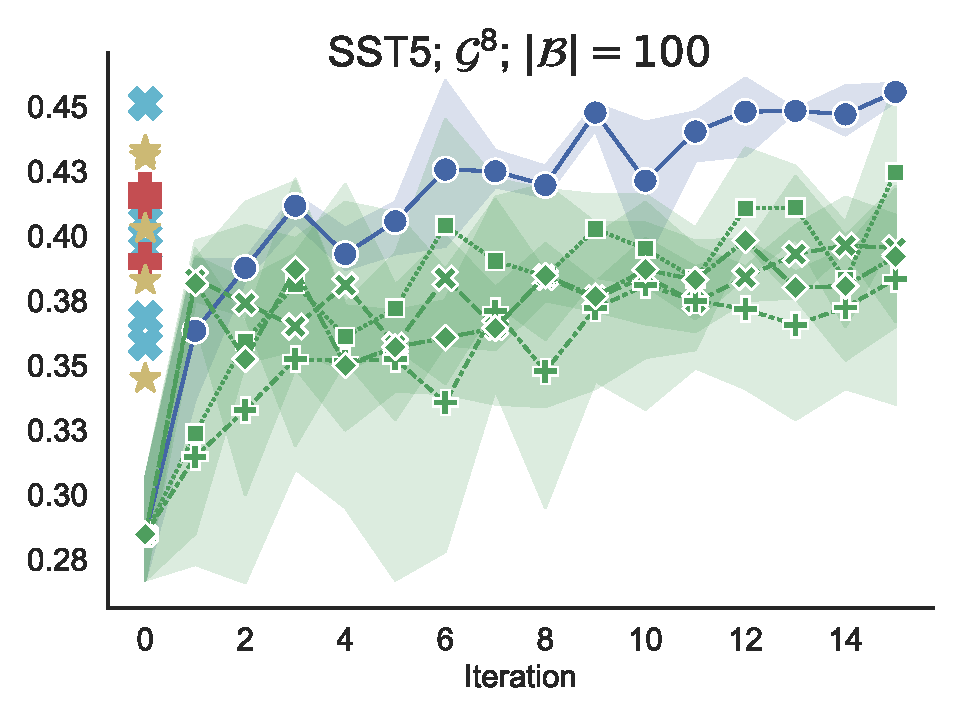
\includegraphics[width=.5\linewidth,height=0.2\textwidth]{imgs/_sst5,agg,8,100.pdf}
}
\vspace{-.2cm}\subfloat{
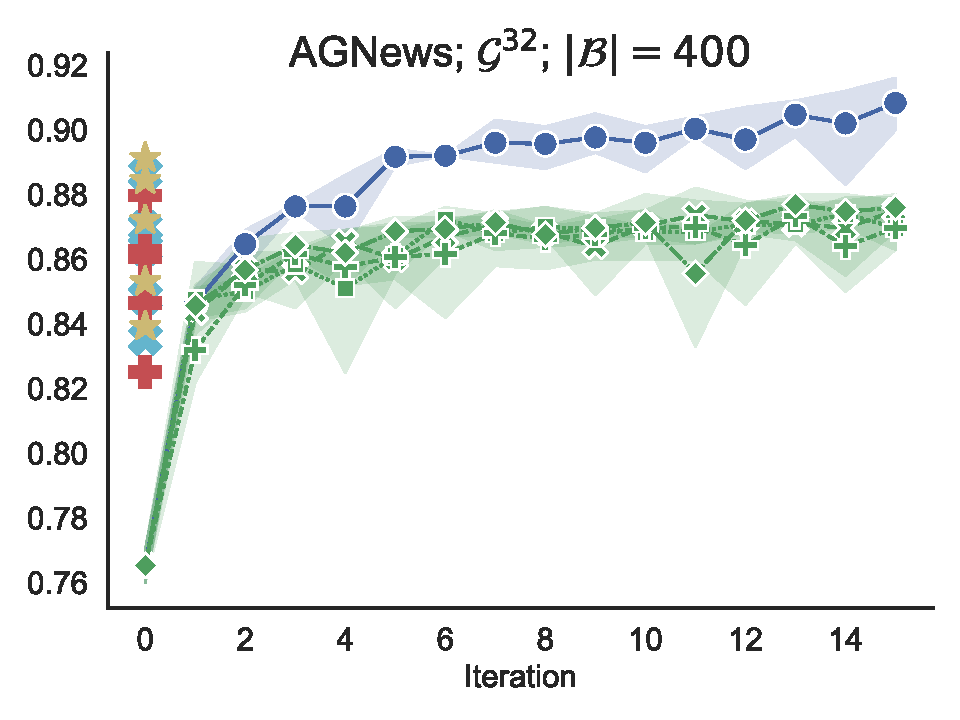
\includegraphics[width=.5\linewidth,height=0.2\textwidth]{imgs/_ag,agg,32,400.pdf}
}
\\
\vspace{-.2cm}\subfloat{
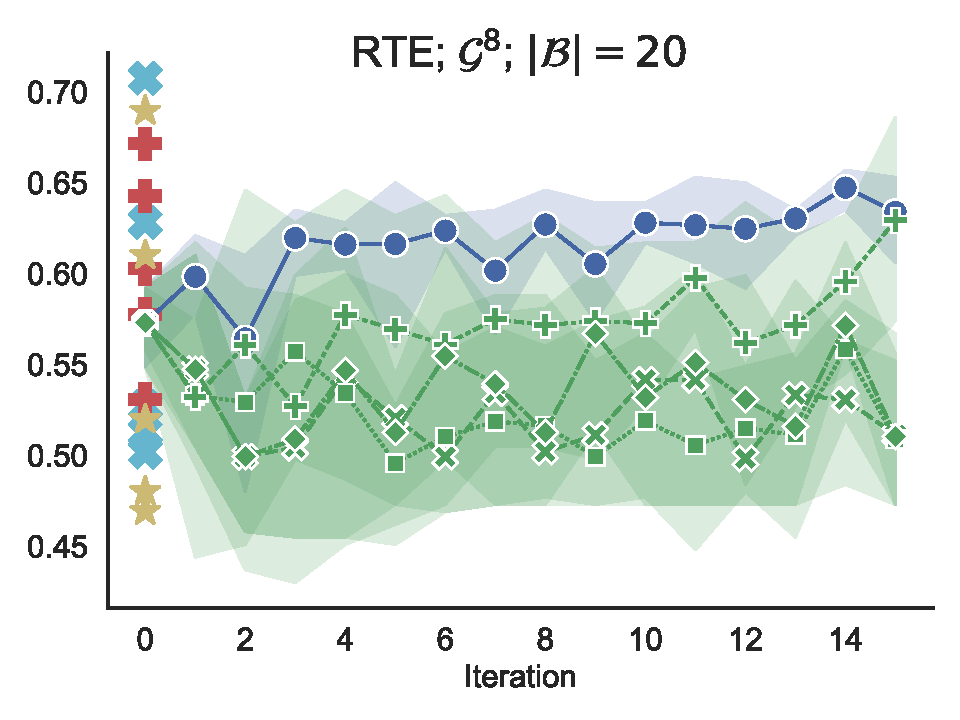
\includegraphics[width=.5\linewidth,height=0.2\textwidth]{imgs/_rte,agg,8,20.pdf}
}
\vspace{-.2cm}\subfloat{
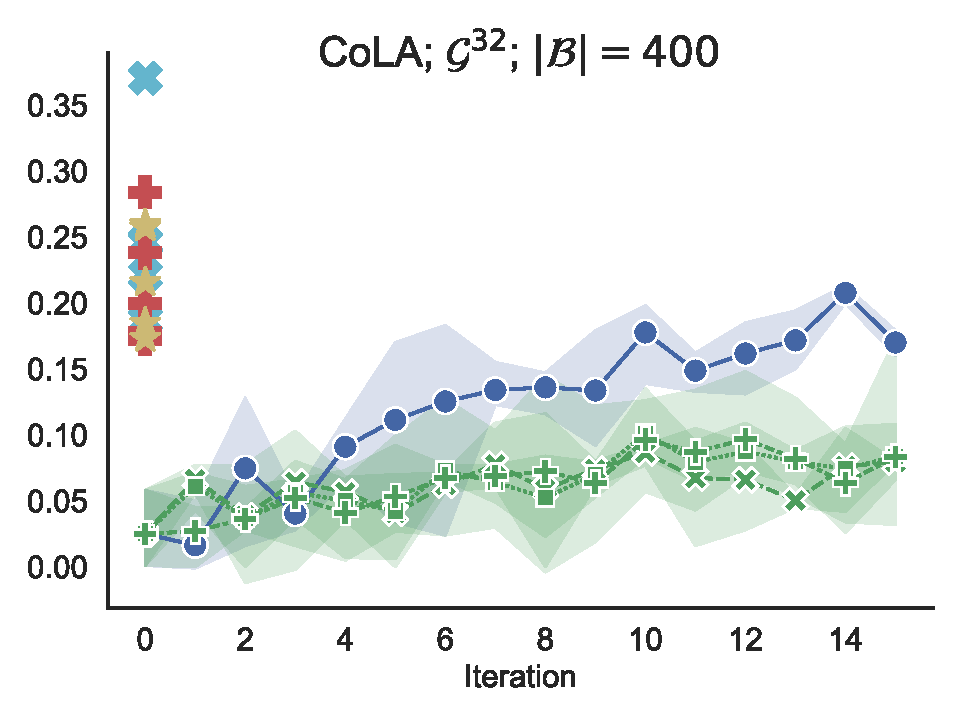
\includegraphics[width=.5\linewidth,height=0.2\textwidth]{imgs/_cola,agg,32,400.pdf}
}
\caption{
  Comparing 
  strategies of aggregating \mdr
  annotations.
  We compare \textcolor{green}{\md (green)} with
  \textcolor{blue}{AL (blue)}.
  Strategies: 
  LogitVoting (\tiny\XSolidBold\normalsize),
  MajorityVoting (\tiny$\blacksquare$\normalsize),
  WeightedLogitVoting (\scriptsize$\blacklozenge$\normalsize),
  BestWorker (\scriptsize\ding{58}\normalsize).  
  AL uses gold labels without aggregation ($\bullet$).
}
\figlabel{varyaggs}
\end{figure}





\subsection{Design choice 1: Aggregation strategies}
\seclabel{varyaggregations}
\figref{varyaggs} compares effectiveness
of different strategies of
aggregating
\mdr annotations
(\secref{subsec:aggregateannotations}).
Looking at 
SST5 and AGNews results (top two images),
we observe that
committee-style aggregation
(LogitVoting (\tiny\XSolidBold\normalsize),
MajorityVoting (\tiny$\blacksquare$\normalsize),
and WeightedLogitVoting (\scriptsize$\blacklozenge$\normalsize))
generally outperforms
BestWorker (\scriptsize\ding{58}\normalsize), which
simply relies on
the
\mdr performing best on $\mathcal{G}_{dev}$.
\mdrs perform well
on these two datasets
as shown by the free markers
at iteration zero;
ensembling their
predictions results in
higher-quality datasets.

In contrast,
BestWorker (\scriptsize\ding{58}\normalsize)
has stellar performance
on RTE (bottom-left),
outperforming
committee-style aggregation.
Note that
even the \mdrs
do not perform
really well in this experiment, as shown
by the free markers at iteration zero --
some \mdrs even
perform worse than $\mathcal{S}$.
Ensembling these low-quality annotations
seems a worse option than simply
relying on the best \mdr.
For CoLA, we observe comparable
performance of different aggregation
strategies.


\begin{figure}[t]
\centering
\subfloat{
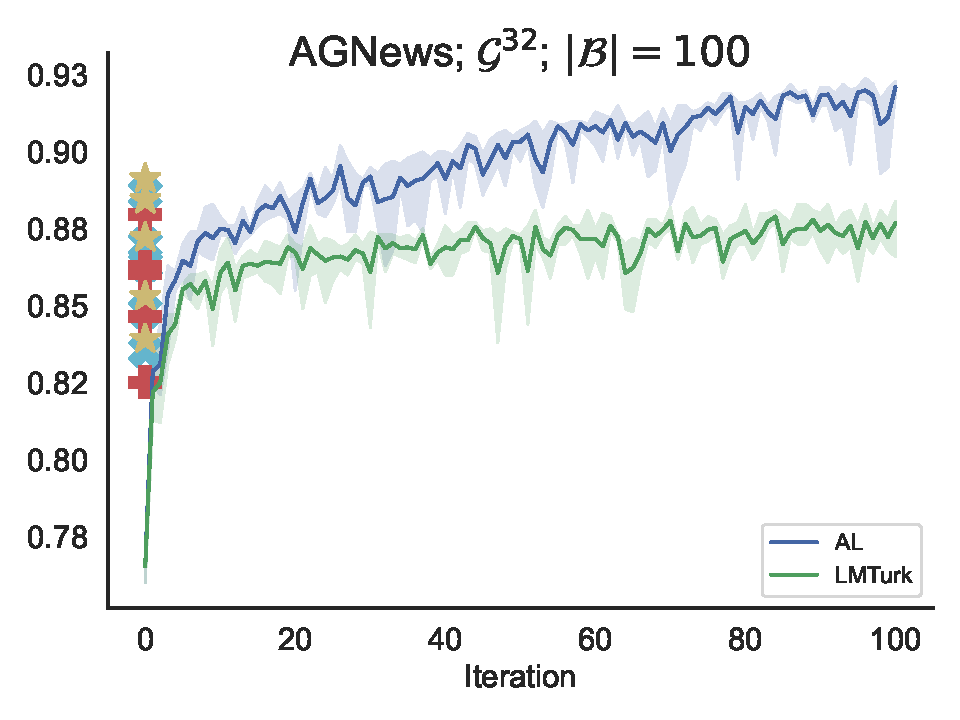
\includegraphics[width=.5\linewidth,height=0.2\textwidth]{imgs/_long,100,100,weightedlogitsvote,as,agnews.pdf}
}
\vspace{-.15cm}\subfloat{
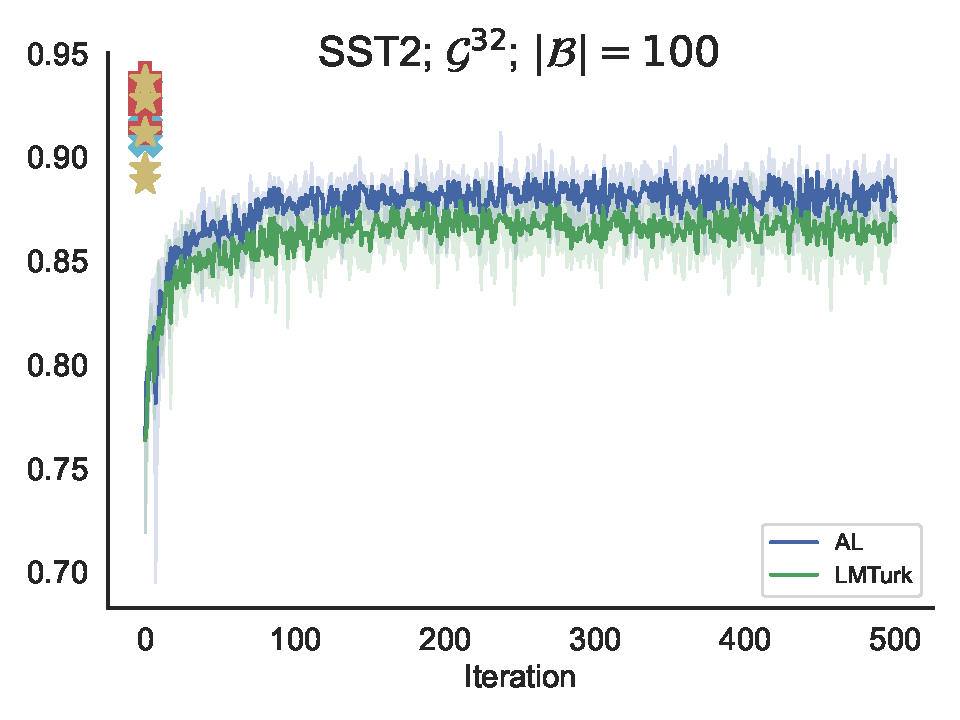
\includegraphics[width=.5\linewidth,height=0.2\textwidth]{imgs/_long,500,100,weightedlogitsvote,as,sst2.pdf}
}
\caption{
  Running more iterations 
  of improving $\mathcal{S}$ with AL and \md.
  Sampling strategy Entropy is used for both methods;
  WeightedLogitVoting is used for aggregating
  \mdr annotations.
}
\figlabel{moreiters}
\end{figure}

\subsection{Design choice 2: More iterations}
We hypothesize that AL performance is an upper bound for
performance when $\mathcal{S}$
is trained with
\mdr annotations -- recall that the AL annotations are gold labels.
\figref{moreiters} compares
AL and \md when running
100 iterations of improving $\mathcal{S}$ on AGNews
and
500 iterations on SST2.
As expected, AL
outperforms \md because
the pool of human-annotated data expands.
The performance of
$\mathcal{S}$ progressively 
approaches that of
the \mdrs; \md performs
comparably to AL in SST2,
however, no human labor is required.



\begin{figure}[t]
\centering
\subfloat{
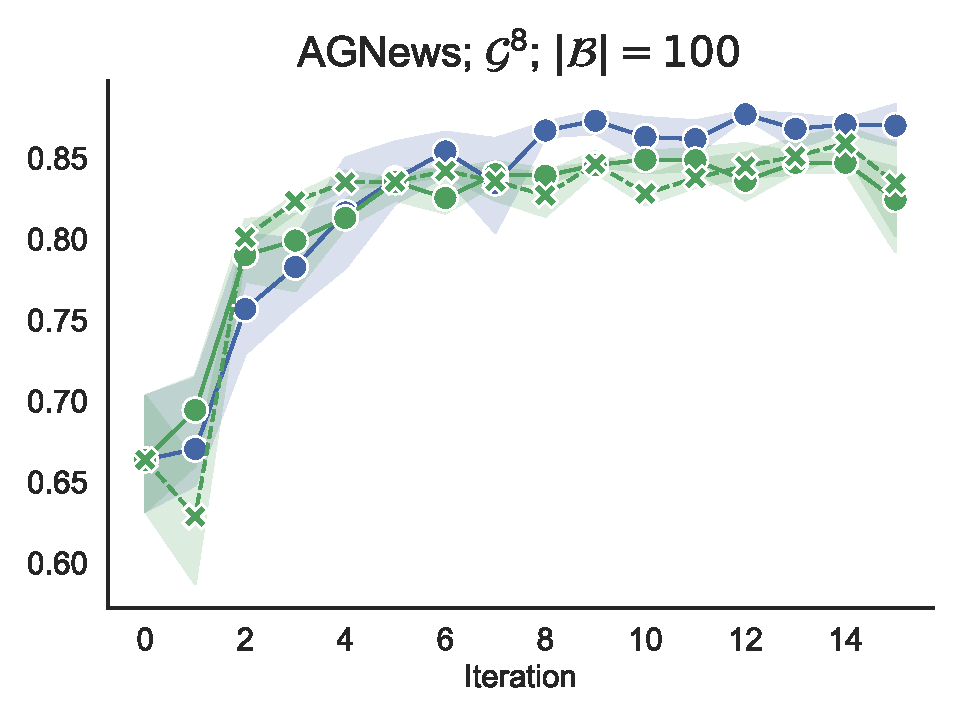
\includegraphics[width=.5\linewidth,height=0.2\textwidth]{imgs/_ag,kl,8,100.pdf}
}
\vspace{-.2cm}\subfloat{
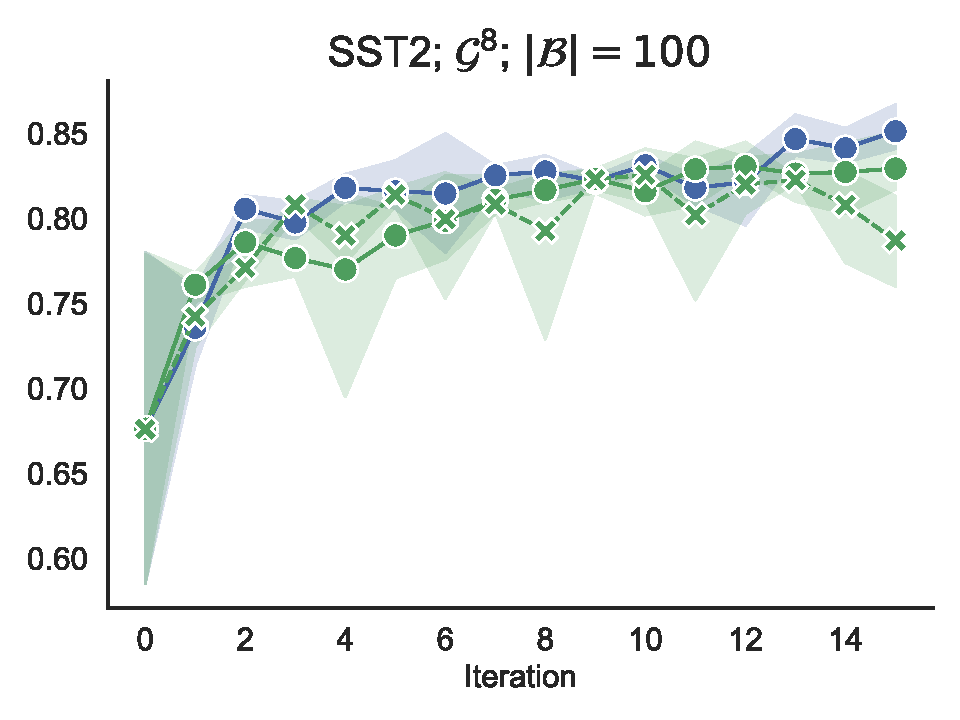
\includegraphics[width=.5\linewidth,height=0.2\textwidth]{imgs/_sst2,kl,8,100.pdf}
}
\\
\vspace{-.2cm}\subfloat{
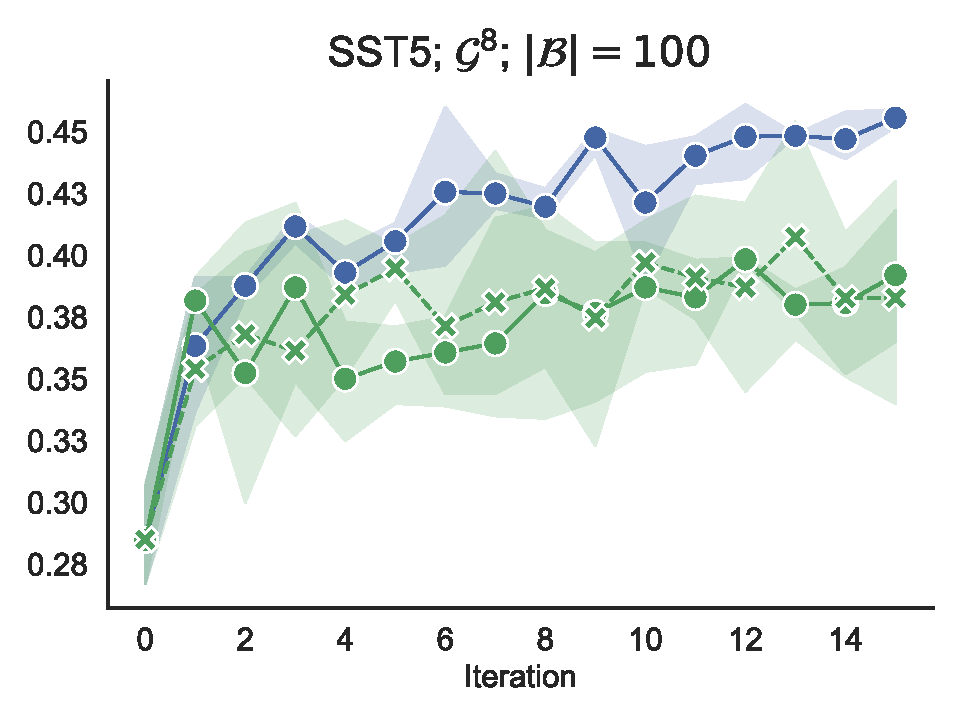
\includegraphics[width=.5\linewidth,height=0.2\textwidth]{imgs/_sst5,kl,8,100.pdf}
}
\vspace{-.2cm}\subfloat{
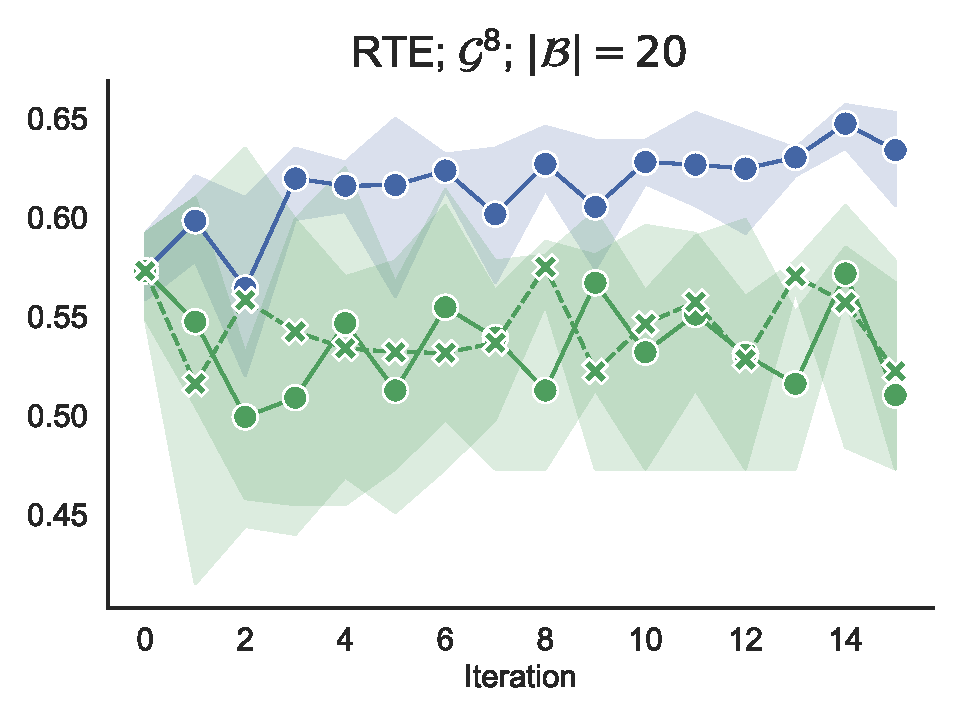
\includegraphics[width=.5\linewidth,height=0.2\textwidth]{imgs/_rte,kl,8,20.pdf}
}
\caption{
  Performance of \textcolor{blue}{AL}
  and \textcolor{green}{\md}
  with  discrete labels ($\bullet$) vs.\
  with KL divergence (\tiny\XSolidBold\normalsize).
  Entropy is used as the sampling strategy
  and WeightedLogitVoting is used 
  to aggregate worker annotations.
}
\figlabel{kllogits}
\end{figure}


\subsection{Design choice 3: Distilling logits}
We can view \md as a kind of distillation \citep{hinton2015distilling}:
The ability of
\mdrs to solve $\mathcal{T}$ is progressively transferred 
to $\mathcal{S}$.
In this section, we explore 
the utility of distillation:
We train
$\mathcal{S}$
with predicted logits\footnote{
Distilling with intermediate activations likely
to further improve performance of $\mathcal{S}$.
However, note that PLM intermediate activations
are not always available in a
Language-Model-as-a-Service framework.
}
instead of discrete labels
from \mdrs.
Concretely, we 
train
$\mathcal{S}$ by reducing the
KL divergence between its
predicted probability distribution
(over the label set)
and the
probability distribution
from \mdrs.

\figref{kllogits} shows that
training
$\mathcal{S}$ with KL divergence
noticeably improves
over discrete labels
on AGNews and SST5.
This is expected:
AGNews and SST5 have larger
label set size (four and five)
such that the
probability distribution over the label set
is more informative than
that of
the binary classification tasks
SST2 and RTE.




\begin{figure}[t]
\centering
\subfloat{
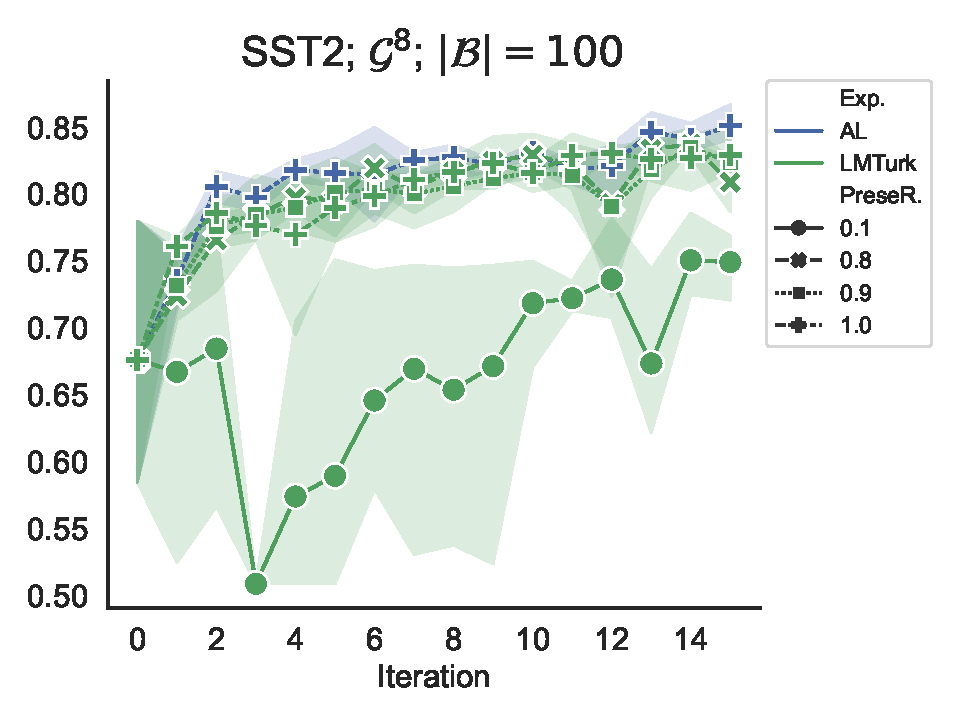
\includegraphics[width=.5\linewidth,height=0.2\textwidth]{imgs/_pooledperfomance,weightedlogitsvote,entropy,as,sst2.pdf}
}
\vspace{-.25cm}\subfloat{
\hspace{-.25cm}
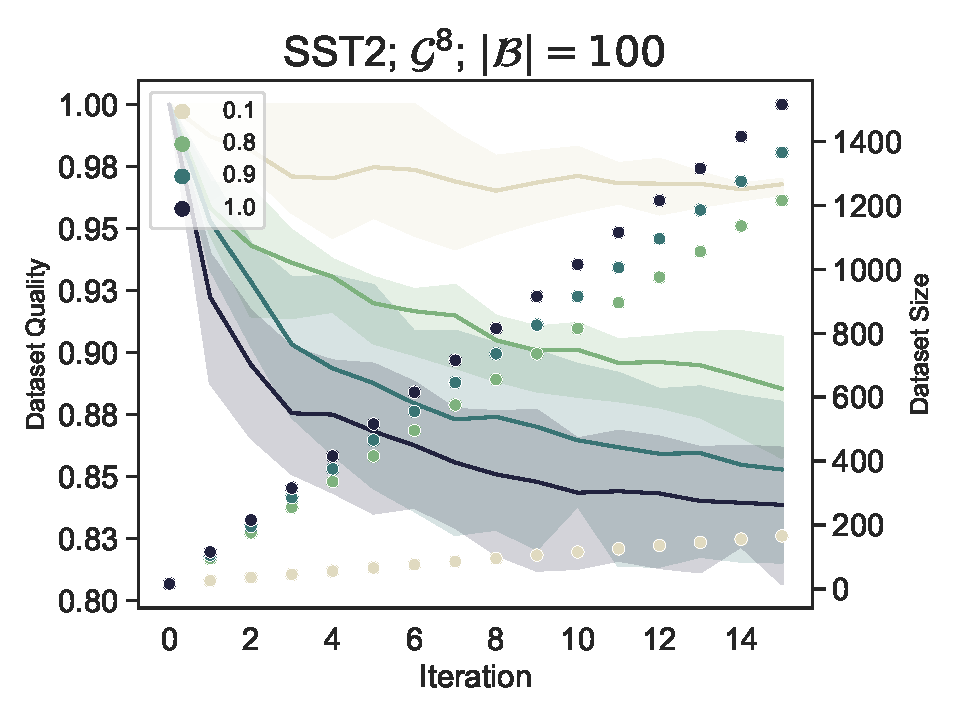
\includegraphics[width=.5\linewidth,height=0.2\textwidth]{imgs/_poolstatus,weightedlogitsvote,entropy,as,sst2.pdf}
}
\\
\vspace{-.25cm}\subfloat{
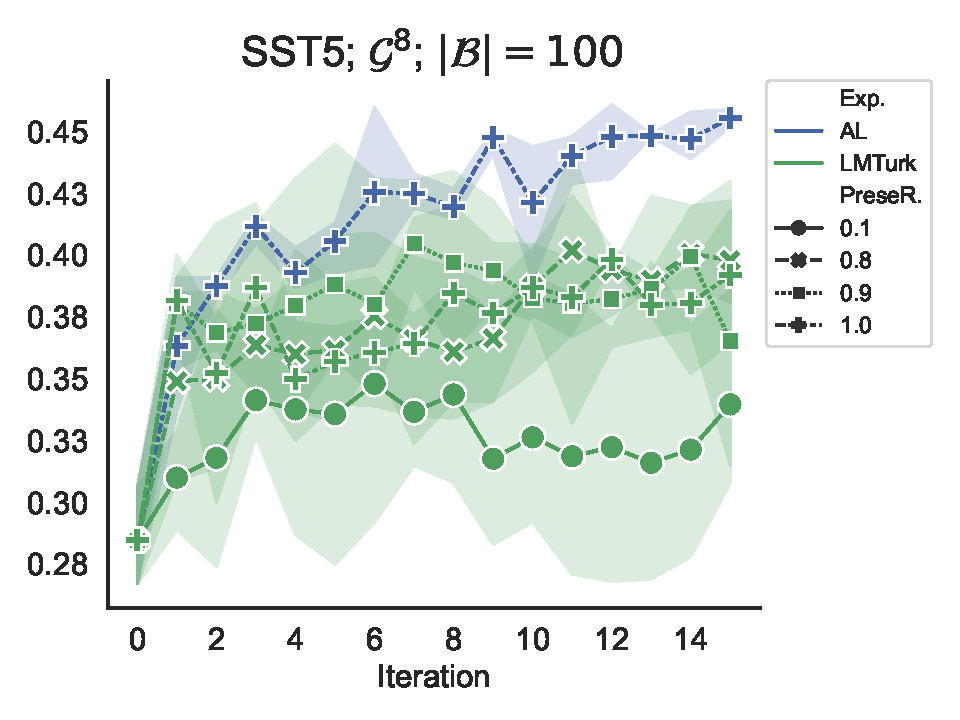
\includegraphics[width=.5\linewidth,height=0.2\textwidth]{imgs/_pooledperfomance,weightedlogitsvote,entropy,as,sst5.pdf}
}
\vspace{-.25cm}\subfloat{
\hspace{-.25cm}    
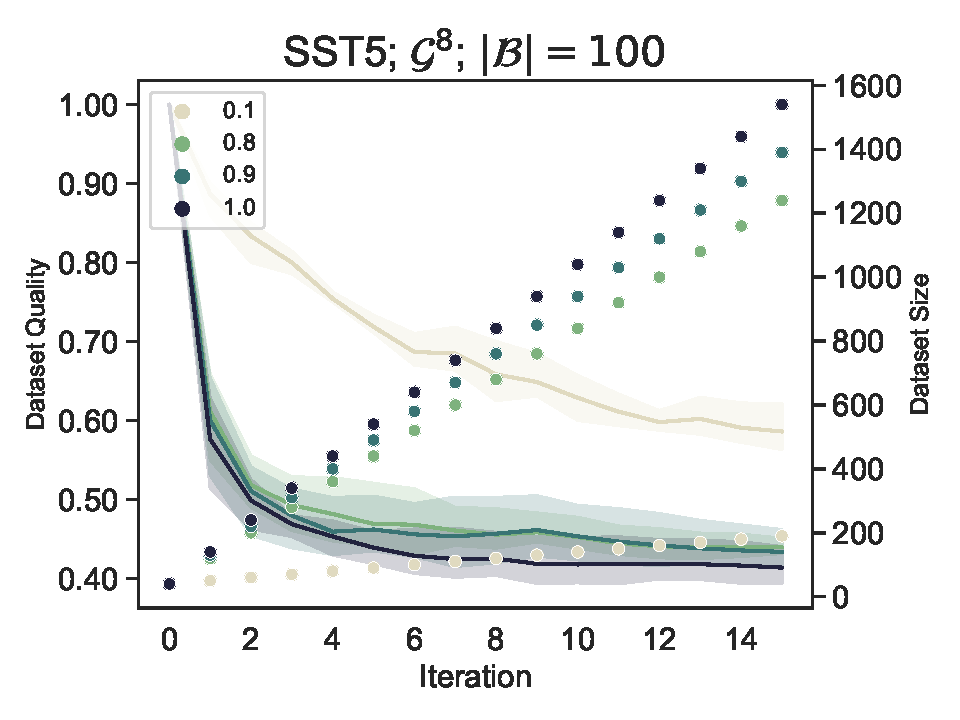
\includegraphics[width=.5\linewidth,height=0.2\textwidth]{imgs/_poolstatus,weightedlogitsvote,entropy,as,sst5.pdf}
}
\\
\vspace{-.25cm}\subfloat{
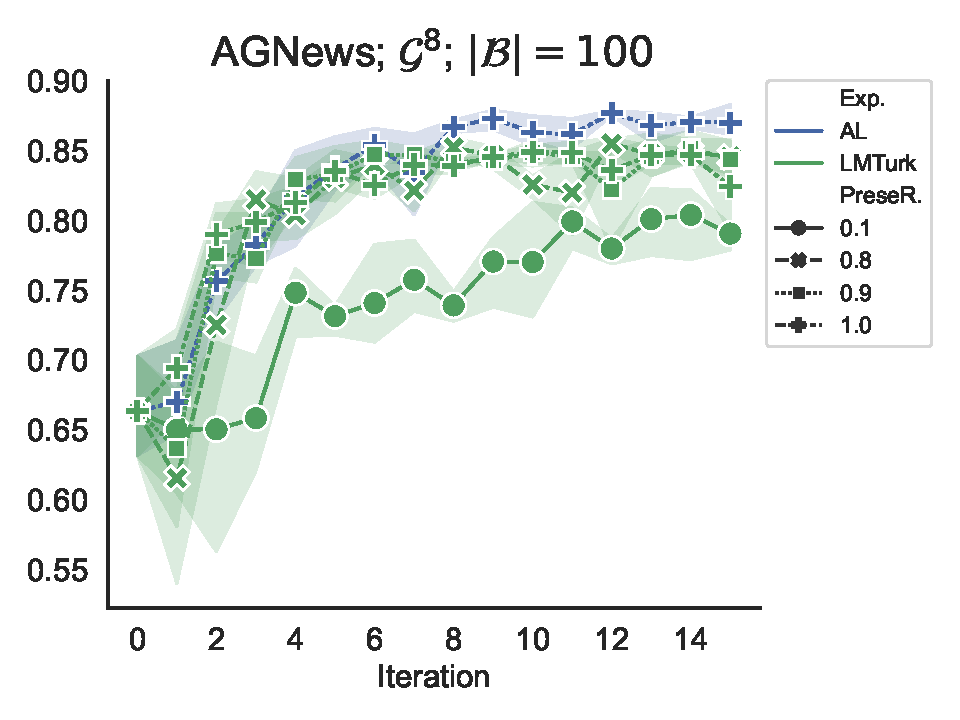
\includegraphics[width=.5\linewidth,height=0.2\textwidth]{imgs/_pooledperfomance,weightedlogitsvote,entropy,as,agnews.pdf}
}
\vspace{-.25cm}\subfloat{
\hspace{-.25cm}  
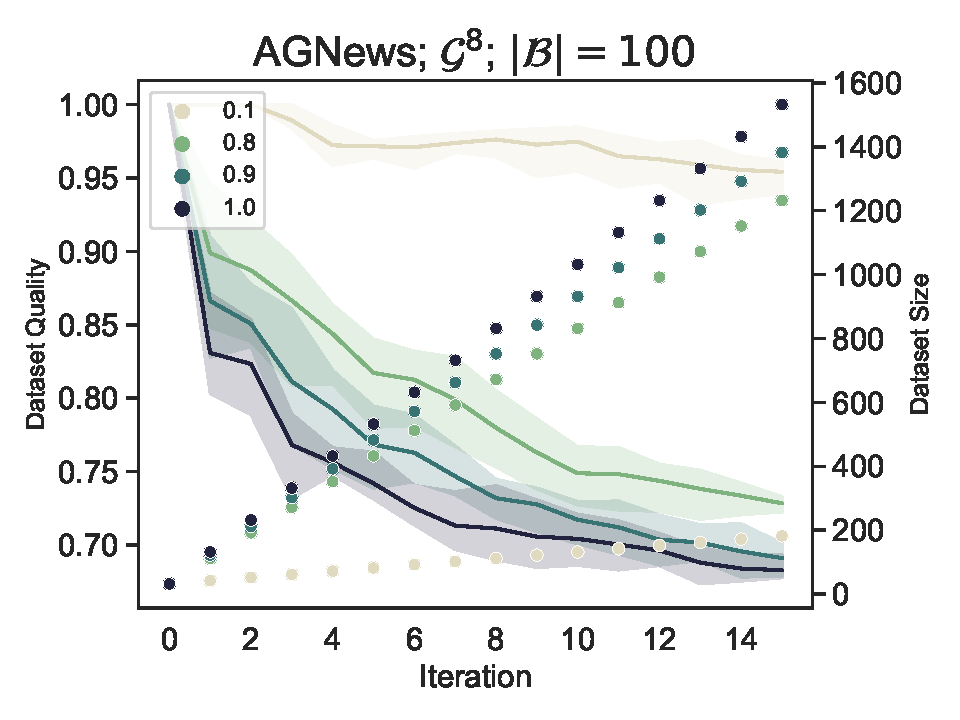
\includegraphics[width=.5\linewidth,height=0.2\textwidth]{imgs/_poolstatus,weightedlogitsvote,entropy,as,agnews.pdf}
}
\caption{
  Training $\mathcal{S}$
  with
  examples for which \mdrs have low entropy.
  We report performance of $\mathcal{S}$ (left),
  number and quality (measured by accuracy) of the
  preserved examples (right) at each iteration.
}
\figlabel{filtering}
\end{figure}




\subsection{Design choice 4: Quality-based filtering}
\seclabel{poolfilter}
One key difference between AL and \md
is that \mdrs are not oracles:
Their labels are not perfect.
Hence, it is reasonable to
consider processing the training
data, denoted as $\mathcal{D}^{j}$, for $\mathcal{S}^{j}$, instead
of using it indiscriminately as in AL.


\textbf{InstanceTresholding} (\secref{instancetresholdingintro})
preserves
annotations
in $\mathcal{D}^{j}$
for which \mdrs
have the smallest
prediction entropy.
Concretely,
we rank all annotations
$(\mathbf{x}, \hat{y}, \mathbf{l}) \in \mathcal{D}^{j}$
by \emph{entropy}($\mathbf{l}$)
and then keep the
$\tau$ percent smallest.
Note that we always preserve the human-labeled
few-shot data $\mathcal{G}_{train}$.
We experiment
with $\tau \in$
\{10\%, \ldots, 90\%, 100\%\}.

\figref{filtering} left shows the
performance of $\mathcal{S}$;
\figref{filtering} right 
tracks the status of
$\mathcal{D}^{j}$.
To measure quality, we compute the accuracy
of \mdr annotations
on $\mathcal{D}^{j}$ (compared to gold labels);
see the lineplots and the left y-axis.
We also report the size
of $\mathcal{D}^{j}$ as
scatter plots (right y-axis).


We observe 
that $\tau$=10\%, i.e., keeping only
the 10\% most certain examples,
gives the worst performance.
This is most obvious at iteration three
for  SST2: The performance
drops to near the majority baseline ($\approx$50\%).
This is because $\mathcal{D}^{3}$
is small and unbalanced: It has
eight negative (from $\mathcal{G}^{train}$)
and 38 positive examples.
However, using
all the \mdr annotations
($\tau$=100\%) may not
be optimal either.
This is noticeable
when looking at SST5:
$\tau$=90\% and $\tau$=80\%
are better options.


We see that there is a trade-off between
$\mathcal{D}^{j}$'s quality and size
from \figref{filtering} right.
Being conservative, i.e.,
preserving
only a handful of
annotations from
\mdrs, results in a small, but high-quality
$\mathcal{D}^{j}$;
using all the annotations
indiscriminately leads to a 
large $\mathcal{D}^{j}$ with low quality.
This experiment
highlights a key difference
between \md and AL:
\mdr annotations 
are not perfect and
taking the annotation quality
into consideration when training 
$\mathcal{S}$ is crucial.


\section{Conclusion}
In this work, our focus is the research
question: \emph{
  How to make effective use
  of current few-shot learners?
} We propose \md,
a simple yet effective method 
that considers PLM-based few-shot learners
as non-expert annotators in crowdsourcing;
active learning strategies are incorporated
to reduce the cost of annotation.
We further show that
processing the annotations from \mdrs
can  be beneficial.

Future work may combine
\mdr annotations with 
human annotators in a human-in-the-loop setup \cite{monarch2021human} to increase the overall utility
of invested resources \citep{bai2021pre}.
Scaling up to even larger PLMs
likely to further
boost model performances \citep{kaplan2020scaling,GPT3paper}
Applying \md to
multilingual few-shot
learners \citep{zhao-etal-2021-closer,winata2021language,lin2021few}
is also
promising.

\section*{Acknowledgements}
We thank the anonymous reviewers for their insightful comments and suggestions.
MZ and HS were supported by the European Research Council
(ERC\# 740516)
and the 
German Federal Ministry of Education and
Research (BMBF, grant \#01IS18036A).




\bibliography{custom}
\clearpage
\appendix
\section{Additional Results}
\subsection{GPT-3 Experiments} 
\label{sec:gpt3}
\begin{table}[ht]
    \centering
\begin{tabular}{c | cc}
\toprule
 & PaLM-540B & GPT-3 \\ \midrule
HotpotQA (exact match) & 29.4 & \textbf{30.8} \\
ALFWorld (success rate \%) & 70.9 & \textbf{78.4} \\ 
\bottomrule
\end{tabular}%
    \caption{\model{} prompting results using PaLM-540B vs.\,GPT-3 (text-davinci-002, greedy decoding). On HotpotQA, we randomly sample a subset of 500 validation questions. On ALFWorld, we use all 134 unseen validation task instances, and use the best prompt set according to PaLM-540B.}
    \label{tab:gpt3}
\end{table}
We run additional GPT-3~\citep{brown2020language} experiments to confirm \model{} prompting performance is general across different large language models. As shown in Table~\ref{tab:gpt3}, GPT-3 (text-davinci-002, greedy decoding) consistently outperforms PaLM-540B on HotpotQA and ALFWorld, possibly because it is finetuned with human instruction following. This indicates ReAct prompting is effective across different large language models on different tasks.
The code for these experiments are at \url{https://react-lm.github.io/}.
\subsection{\model{} obtains up-to-date knowledge on HotpotQA}
\begin{figure}[ht]
    \centering
    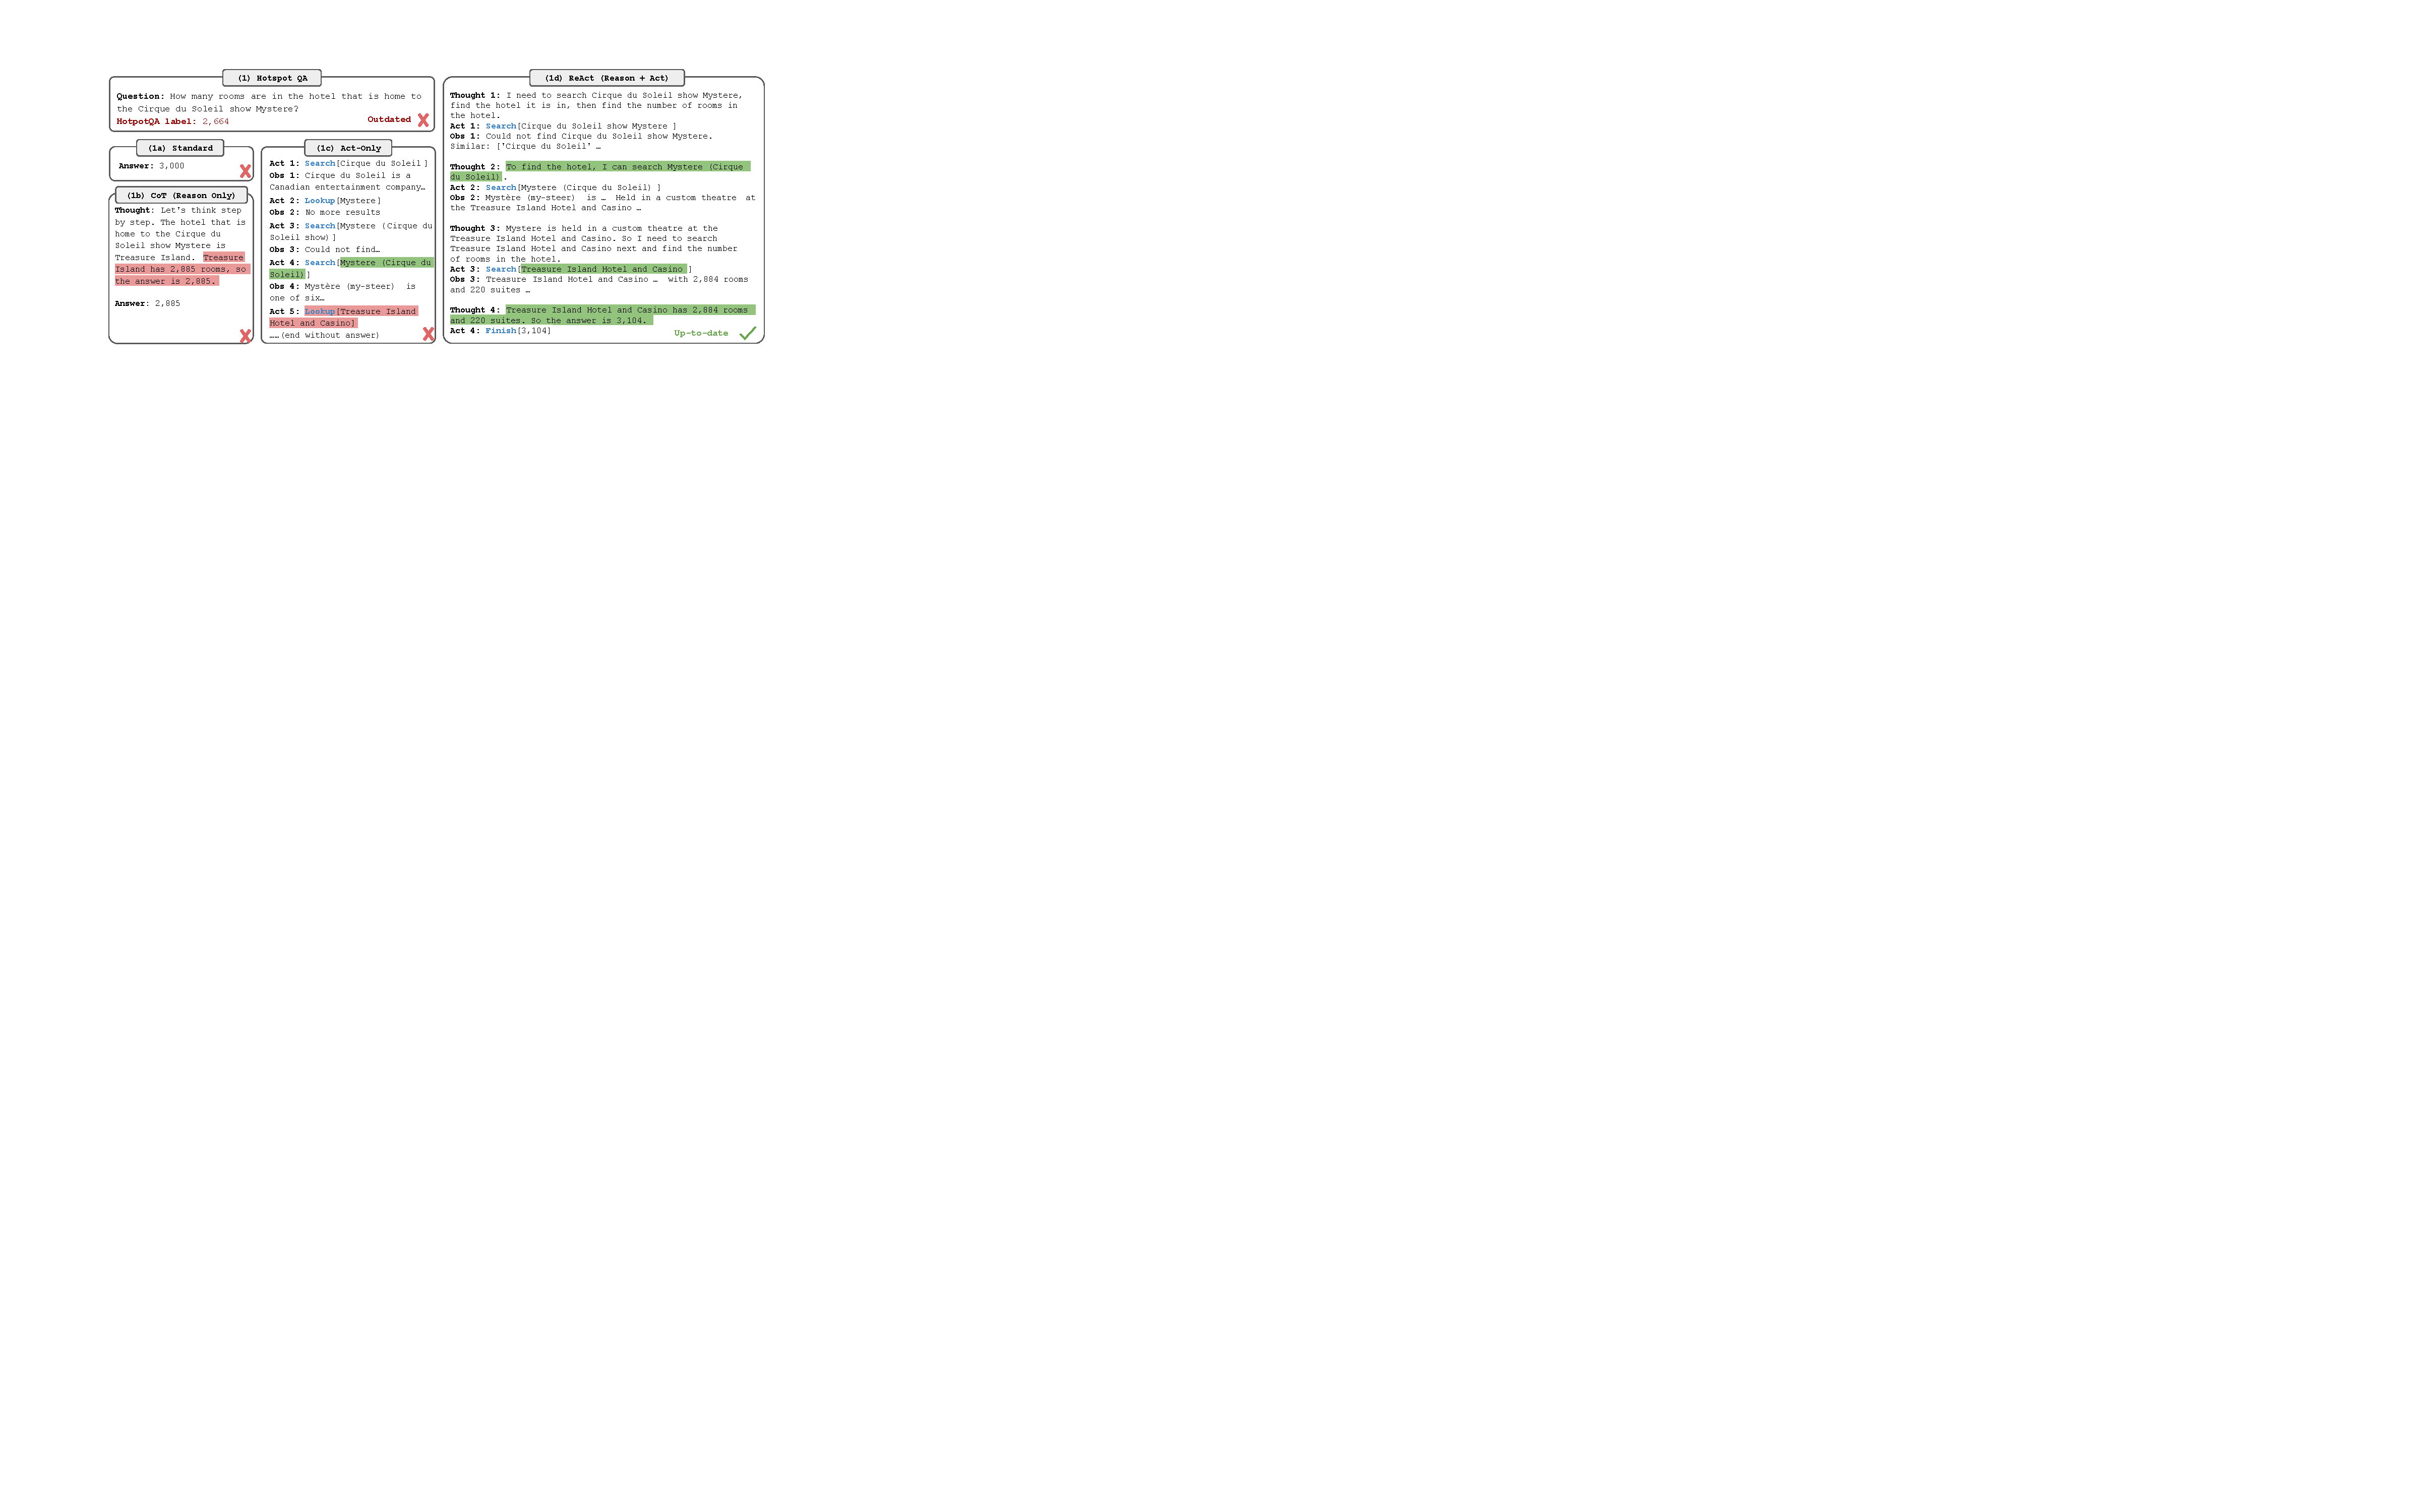
\includegraphics[width=\textwidth]{iclr2023/figure/date.pdf}
    \caption{
    {
    Another example HotpotQA question, where the original label is outdated. Only \model{} is able to obtain the up-to-date answer thanks to real-world web interaction plus reasoning.}
    }
    \label{fig:date}
    \vspace{-10pt}
\end{figure}

During trajectory inspection, we also find that sometimes \model{} does not agree with dataset labels as the labels themselves could be outdated. For example, as shown in Figure~\ref{fig:date}, the question asks about the size of a hotel, which increased from the HotpotQA construction time. While \palm{} and \reason{} give wrong answers due to hallucination, \act{} fails despite the access of real-world web interaction, due to a lack of reasoning to guide how to interact with the Internet for QA. Only \model{} is able to retrieve up-to-date information from the Internet and provide a reasonable answer. Therefore, better incorporation of reasoning abilities might benefit recent Internet-augmented language models~\citep{nakano2021webgpt,lazaridou2022internet,shuster2022language} for up-to-date task solving. 
\subsection{Human-in-the-loop behavior correction on AlfWorld} 
\begin{figure}[ht]
    \centering
    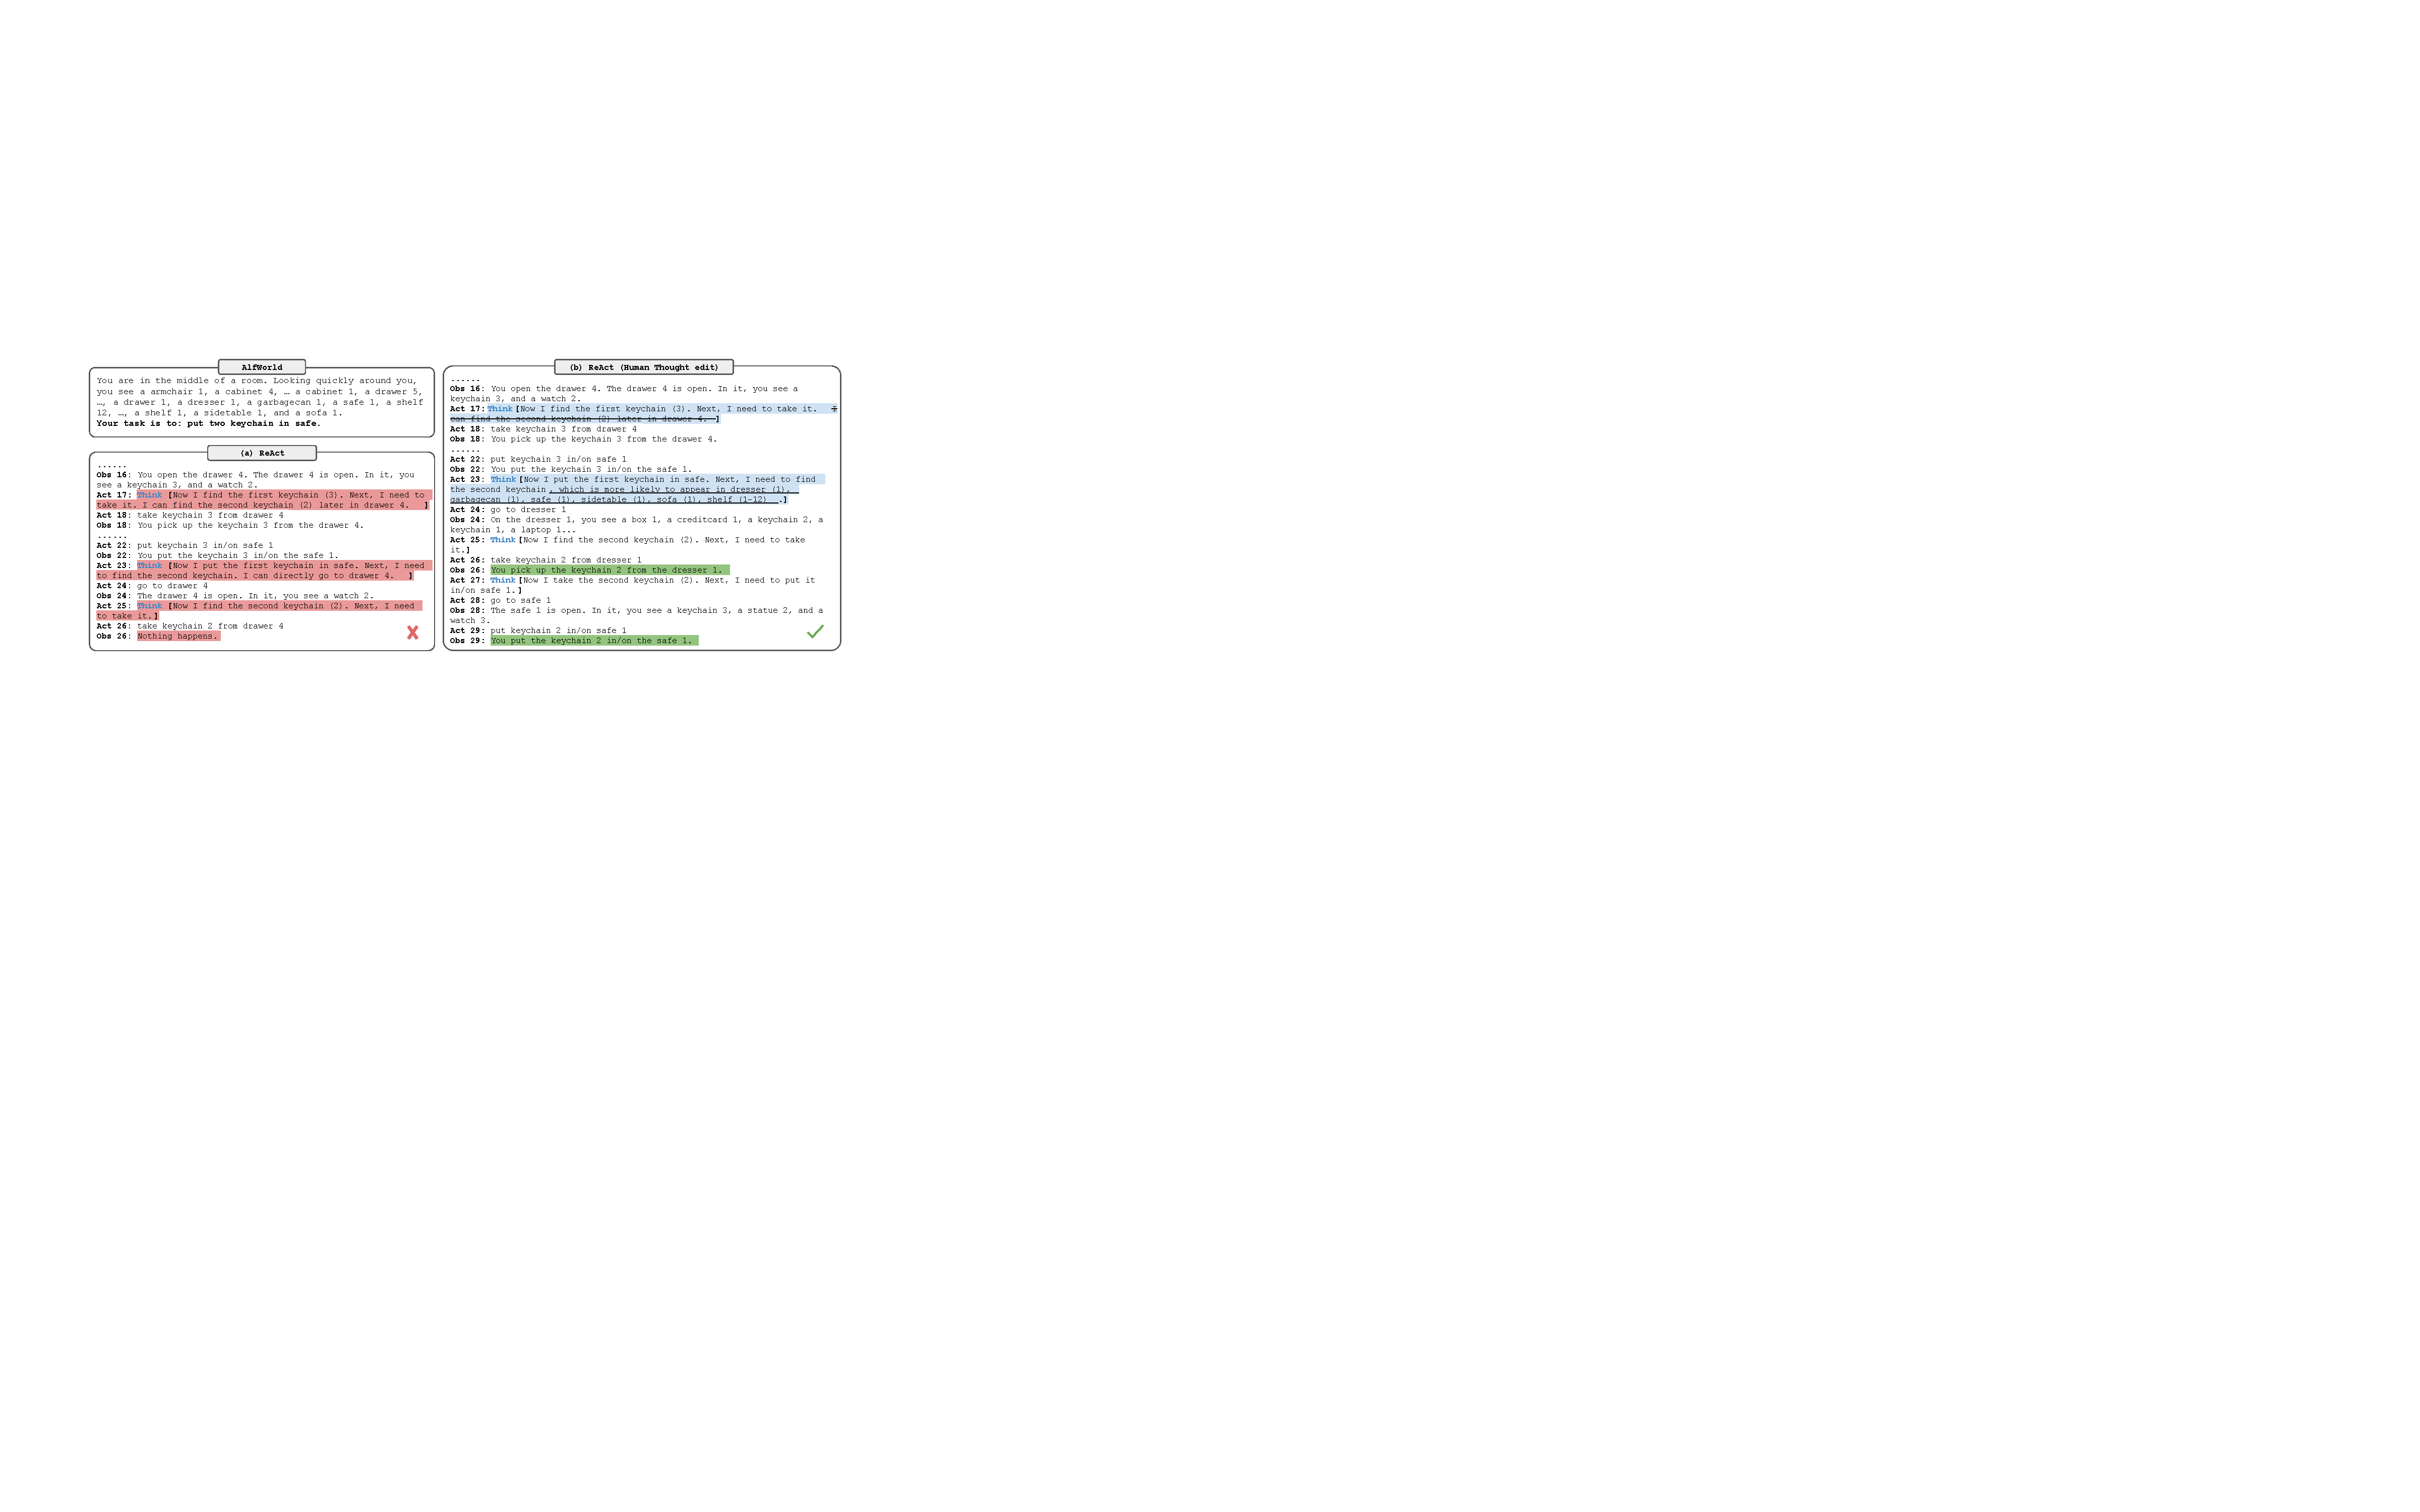
\includegraphics[width=\textwidth]{iclr2023/figure/human_edit.pdf}
    \caption{
    A human-in-the-loop behavior correction example with \model{} in AlfWorld. 
    (a) \model{} trajectory fails due to a hallucinating thought (Act 17).
    (b) By a human simply editing two thoughts (Act 17, 23), the \model{} trajectory produces desirable reasoning traces and actions and succeeds.
    }
    \label{fig:edit}
    \vspace{-10pt}
\end{figure}

We also explore human-in-the-loop interaction with \model{}, to allow a human to inspect and edit \model's reasoning traces. Figure~\ref{fig:edit} shows that
by simply removing a hallucinating sentence in Act 17 and adding some hints in Act 23, \model{} can be made to change its behavior drastically to align with these human thought edits and succeed in the task. 
From a human perspective, solving such a task becomes significantly easier, from typing tens of actions to only editing a couple of thoughts, which enables new forms of human-machine collaboration.
We note that such a policy edit on-the-go is difficult for \act{} and previous RL methods, as a human cannot change the model parameters, and changing a few actions might not edit the rest of the model behavior. 
This paradigm is also more than human dialogue to update the goal or subgoal as in \citet{huang2022inner} --- while editing \model{} thoughts can do these, it can also modify the model's internal belief, reasoning styles, or anything the flexible thought space supports, for better task solving. 
We believe this is an exciting direction for human alignment and leave more systematic study as future work.

\section{Experiment Details}
\subsection{HotpotQA Finetuning Details}
\label{sec:hotpot_finetune}
For all finetuning we use a batch size of 64.
On PaLM-8B, we finetune \model{} and \act{} methods for $4,000$ steps and \palm{} and \reason{} methods for $2,000$ steps. 
On PaLM-62B, we finetune \model{} and \act{} methods for $4,000$ steps and \palm{} and \reason{} methods for $1,000$ steps. 
We find \model{} and \act{} methods generally benefit from more training steps (and more training data), while  \palm{} and \reason{} methods degrade soon after finetuning.

\subsection{AlfWorld IM-Style Details}
\label{sec:alfworld_im}
For the IM-style ablation, the same expert trajectories used in \model{} are reannotated with dense external feedback thoughts within these trajectories, that limit \modelim{} to only think about (1) decomposing the current goal and (2) the current subgoal that needs to be completed. In particular, \modelim{} lacks thoughts that (1) determine when a subgoal is completed (2) determine what the next subgoal should be (3) inducing the LLM to refer to its internal pretraining knowledge to identify where items can be within the environment. 


\section{Prompts}
\label{sec:prompts}
\subsection{HotpotQA}
\begin{table}[H]
\scriptsize
\begin{minipage}{0.9\linewidth}
Hotpot QA Prompts
\centering
\ttfamily
\begin{tabular}{l p{0.9\linewidth}}
\midrule
\sethlcolor{cyan}\hl{Original} & \\
Question &  What is the elevation range for the area that the eastern sector of the Colorado orogeny extends into? \\
Answer &  1,800 to 7,000 ft\\
\\
Question &  Musician and satirist Allie Goertz wrote a song about the "The Simpsons" character Milhouse, who Matt Groening named after who?\\
Answer &  Richard Nixon\\
\\
Question &  Which documentary is about Finnish rock groups, Adam Clayton Powell or The Saimaa Gesture?\\
Answer &  The Saimaa Gesture\\
\\
Question &  What profession does Nicholas Ray and Elia Kazan have in common?\\
Answer &  director, screenwriter, actor\\
\\
Question &  Which magazine was started first Arthur's Magazine or First for Women?\\
Answer &  Arthur's Magazine\\
\\
Question &  Were Pavel Urysohn and Leonid Levin known for the same type of work?\\
Answer &  Yes\\


\midrule
\sethlcolor{red}\hl{\act} & \\
Question &  What is the elevation range for the area that the eastern sector of the Colorado orogeny extends into?\\
Action 1 &  Search[Colorado orogeny]\\
Observation 1 &  The Colorado orogeny was an episode of mountain building (an orogeny) in Colorado and surrounding areas.\\
Action 2 &  Lookup[eastern sector]\\
Observation 2 &  (Result 1 / 1) The eastern sector extends into the High Plains and is called the Central Plains orogeny.\\
Action 3 &  Search[High Plains]\\
Observation 3 &  High Plains refers to one of two distinct land regions: \\
Action 4 &  Search[High Plains (United States)]\\
Observation 4 &  The High Plains are a subregion of the Great Plains. From east to west, the High Plains rise in elevation from around 1,800 to 7,000 ft (550 to 2,130 m).[3]\\
Action 5 &  Finish[1,800 to 7,000 ft]\\
\\
Question &  Musician and satirist Allie Goertz wrote a song about the "The Simpsons" character Milhouse, who Matt Groening named after who?\\
Action 1 &  Search[Milhouse]\\
Observation 1 &  Milhouse Mussolini Van Houten is a recurring character in the Fox animated television series The Simpsons voiced by Pamela Hayden and created by Matt Groening.\\
Action 2 &  Lookup[named after]\\
Observation 2 &  (Result 1 / 1) Milhouse was named after U.S. president Richard Nixon, whose middle name was Milhous. \\
Action 3 &  Finish[Richard Nixon]\\
\\
Question &  Which documentary is about Finnish rock groups, Adam Clayton Powell or The Saimaa Gesture?\\
Action 1 &  Search[Adam Clayton Powell]\\
Observation 1 &  Could not find [Adam Clayton Powell]. Similar:  ['Adam Clayton Powell III', 'Seventh Avenue (Manhattan)', 'Adam Clayton Powell Jr. State Office Building', 'Isabel Washington Powell', 'Adam Powell', 'Adam Clayton Powell (film)', 'Giancarlo Esposito'].\\
Action 2 &  Search[Adam Clayton Powell (film)]\\
Observation 2 &  Adam Clayton Powell is a 1989 American documentary film directed by Richard Kilberg. The film is about the rise and fall of influential African-American politician Adam Clayton Powell Jr.[3][4] It was later aired as part of the PBS series The American Experience.\\
Action 3 &  Finish[The Saimaa Gesture]\\
\\
Question &  What profession does Nicholas Ray and Elia Kazan have in common?\\
Action 1 &  Search[Nicholas Ray]\\
Observation 1 &  Nicholas Ray (born Raymond Nicholas Kienzle Jr., August 7, 1911 – June 16, 1979) was an American film director, screenwriter, and actor best known for the 1955 film Rebel Without a Cause.\\
Action 2 &  Search[Elia Kazan]\\
Observation 2 &  Elia Kazan was an American film and theatre director, producer, screenwriter and actor.\\


\midrule \multicolumn{2}{r}{\textit{Continued on next page}} \\
\end{tabular}
\end{minipage}%
\end{table}


\begin{table}[H]
\scriptsize
\begin{minipage}{0.9\linewidth}
Hotpot QA Prompts -- Continued from previous page
\centering
\ttfamily
\begin{tabular}{l p{0.9\linewidth}}
\midrule
\\
Action 3 &  Finish[director, screenwriter, actor]\\
Question &  Which magazine was started first Arthur's Magazine or First for Women?\\
Action 1 &  Search[Arthur's Magazine]\\
Observation 1 &  Arthur's Magazine (1844--1846) was an American literary periodical published in Philadelphia in the 19th century. \\
Action 2 &  Search[First for Women]\\
Observation 2 &  First for Women is a woman's magazine published by Bauer Media Group in the USA.[1] The magazine was started in 1989. \\
Action 3 &  Finish[Arthur's Magazine]\\
\\
Question &  Were Pavel Urysohn and Leonid Levin known for the same type of work?\\
Action 1 &  Search[Pavel Urysohn]\\
Observation 1 &  Pavel Samuilovich Urysohn (February 3, 1898 - August 17, 1924) was a Soviet mathematician who is best known for his contributions in dimension theory.\\
Action 2 &  Search[Leonid Levin]\\
Observation 2 &  Leonid Anatolievich Levin is a Soviet-American mathematician and computer scientist. \\
Action 3 &  Finish[yes]\\
\midrule
\sethlcolor{green}\hl{\reason} & \\
Question &  What is the elevation range for the area that the eastern sector of the Colorado orogeny extends into?\\
Thought &  Let's think step by step. The eastern sector of Colorado orogeny extends into the High Plains. High Plains rise in elevation from around 1,800 to 7,000 ft, so the answer is 1,800 to 7,000 ft.\\
Answer &  1,800 to 7,000 ft\\
\\
Question &  Musician and satirist Allie Goertz wrote a song about the "The Simpsons" character Milhouse, who Matt Groening named after who?\\
Thought &  Let's think step by step. Milhouse was named after U.S. president Richard Nixon, so the answer is Richard Nixon.\\
Answer &  Richard Nixon\\
\\
Question &  Which documentary is about Finnish rock groups, Adam Clayton Powell or The Saimaa Gesture?\\
Thought &  Let's think step by step. Adam Clayton Powell (film) is a documentary about an African-American politician, not Finnish rock groups. So the documentary about Finnish rock groups must instead be The Saimaa Gesture.\\
Answer &  The Saimaa Gesture\\
\\
Question &  What profession does Nicholas Ray and Elia Kazan have in common?\\
Thought &  Let's think step by step. Professions of Nicholas Ray are director, screenwriter, and actor. Professions of Elia Kazan are director, producer, screenwriter, and actor. So profession Nicholas Ray and Elia Kazan have in common is director, screenwriter, and actor.\\
Answer &  director, screenwriter, actor\\
\\
Question &  Which magazine was started first Arthur's Magazine or First for Women?\\
Thought &  Let's think step by step. Arthur's Magazine was started in 1844. First for Women was started in 1989. 1844 (Arthur's Magazine) < 1989 (First for Women), so Arthur's Magazine was started first.\\
Answer &  Arthur's Magazine\\
\\
Question &  Were Pavel Urysohn and Leonid Levin known for the same type of work?\\
Thought &  Let's think step by step. Pavel Urysohn is a mathematician. Leonid Levin is a mathematician and computer scientist. So Pavel Urysohn and Leonid Levin have the same type of work.\\
Answer &  Yes\\


\midrule
\sethlcolor{yellow}\hl{\model} & \\
Question &  What is the elevation range for the area that the eastern sector of the Colorado orogeny extends into?\\
Thought 1 &  I need to search Colorado orogeny, find the area that the eastern sector of the Colorado orogeny extends into, then find the elevation range of the area.\\
Action 1 &  Search[Colorado orogeny]\\
Observation 1 &  The Colorado orogeny was an episode of mountain building (an orogeny) in Colorado and surrounding areas.\\
Thought 2 &  It does not mention the eastern sector. So I need to look up eastern sector.\\
Action 2 &  Lookup[eastern sector]\\
Observation 2 &  (Result 1 / 1) The eastern sector extends into the High Plains and is called the Central Plains orogeny.\\
Thought 3 &  The eastern sector of Colorado orogeny extends into the High Plains. So I need to search High Plains and find its elevation range.\\
Action 3 &  Search[High Plains]\\
Observation 3 &  High Plains refers to one of two distinct land regions  \\
Thought 4 &  I need to instead search High Plains (United States).\\
Action 4 &  Search[High Plains (United States)]\\

\midrule \multicolumn{2}{r}{\textit{Continued on next page}} \\

\end{tabular}
\end{minipage}%
\end{table}


\begin{table}[H]
\scriptsize
\begin{minipage}{0.9\linewidth}
Hotpot QA Prompts -- Continued from previous page
\centering
\ttfamily
\begin{tabular}{l p{0.9\linewidth}}
\midrule
\\
Observation 4 &  The High Plains are a subregion of the Great Plains. From east to west, the High Plains rise in elevation from around 1,800 to 7,000 ft (550 to 2,130 m).[3]\\
Thought 5 &  High Plains rise in elevation from around 1,800 to 7,000 ft, so the answer is 1,800 to 7,000 ft.\\
Action 5 &  Finish[1,800 to 7,000 ft]\\
\\
Question &  Musician and satirist Allie Goertz wrote a song about the "The Simpsons" character Milhouse, who Matt Groening named after who?\\
Thought 1 &  The question simplifies to "The Simpsons" character Milhouse is named after who. I only need to search Milhouse and find who it is named after.\\
Action 1 &  Search[Milhouse]\\
Observation 1 &  Milhouse Mussolini Van Houten is a recurring character in the Fox animated television series The Simpsons voiced by Pamela Hayden and created by Matt Groening.\\
Thought 2 &  The paragraph does not tell who Milhouse is named after, maybe I can look up "named after".\\
Action 2 &  Lookup[named after]\\
Observation 2 &  (Result 1 / 1) Milhouse was named after U.S. president Richard Nixon, whose middle name was Milhous. \\
Thought 3 &  Milhouse was named after U.S. president Richard Nixon, so the answer is Richard Nixon.\\
Action 3 &  Finish[Richard Nixon]\\
\\
Question &  Which documentary is about Finnish rock groups, Adam Clayton Powell or The Saimaa Gesture?\\
Thought 1 &  I need to search Adam Clayton Powell and The Saimaa Gesture, and find which documentary is about Finnish rock groups.\\
Action 1 &  Search[Adam Clayton Powell]\\
Observation 1 &  Could not find [Adam Clayton Powell]. Similar:  ['Adam Clayton Powell III', 'Seventh Avenue (Manhattan)', 'Adam Clayton Powell Jr. State Office Building', 'Isabel Washington Powell', 'Adam Powell', 'Adam Clayton Powell (film)', 'Giancarlo Esposito'].\\
Thought 2 &  To find the documentary, I can search Adam Clayton Powell (film).\\
Action 2 &  Search[Adam Clayton Powell (film)]\\
Observation 2 &  Adam Clayton Powell is a 1989 American documentary film directed by Richard Kilberg.
The film is about the rise and fall of influential African-American politician Adam Clayton Powell Jr.[3][4] It was later aired as part of the PBS series The American Experience.\\
Thought 3 &  Adam Clayton Powell (film) is a documentary about an African-American politician, not Finnish rock groups. So the documentary about Finnish rock groups must instead be The Saimaa Gesture.\\
Action 3 &  Finish[The Saimaa Gesture]\\
\\
Question &  What profession does Nicholas Ray and Elia Kazan have in common?\\
Thought 1 &  I need to search Nicholas Ray and Elia Kazan, find their professions, then find the profession they have in common.\\
Action 1 &  Search[Nicholas Ray]\\
Observation 1 &  Nicholas Ray (born Raymond Nicholas Kienzle Jr., August 7, 1911 – June 16, 1979) was an American film director, screenwriter, and actor best known for the 1955 film Rebel Without a Cause.\\
Thought 2 &  Professions of Nicholas Ray are director, screenwriter, and actor. I need to search Elia Kazan next and find his professions.\\
Action 2 &  Search[Elia Kazan]\\
Observation 2 &  Elia Kazan was an American film and theatre director, producer, screenwriter and actor.\\
Thought 3 &  Professions of Elia Kazan are director, producer, screenwriter, and actor. So profession Nicholas Ray and Elia Kazan have in common is director, screenwriter, and actor.\\
Action 3 &  Finish[director, screenwriter, actor]\\
\\
Question &  Which magazine was started first Arthur's Magazine or First for Women?\\
Thought 1 &  I need to search Arthur's Magazine and First for Women, and find which was started first.\\
Action 1 &  Search[Arthur's Magazine]\\
Observation 1 &  Arthur's Magazine (1844-1846) was an American literary periodical published in Philadelphia in the 19th century. \\
Thought 2 &  Arthur's Magazine was started in 1844. I need to search First for Women next.\\
Action 2 &  Search[First for Women]\\
Observation 2 &  First for Women is a woman's magazine published by Bauer Media Group in the USA.[1] The magazine was started in 1989. \\
Thought 3 &  First for Women was started in 1989. 1844 (Arthur's Magazine) < 1989 (First for Women), so Arthur's Magazine was started first.\\
Action 3 &  Finish[Arthur's Magazine]\\
\\
Question &  Were Pavel Urysohn and Leonid Levin known for the same type of work?\\
Thought 1 &  I need to search Pavel Urysohn and Leonid Levin, find their types of work, then find if they are the same.\\
Action 1 &  Search[Pavel Urysohn]\\

\midrule \multicolumn{2}{r}{\textit{Continued on next page}} \\



\end{tabular}
\end{minipage}%
\end{table}


\begin{table}[H]
\scriptsize
\begin{minipage}{0.9\linewidth}
Hotpot QA Prompts -- Continued from previous page
\centering
\ttfamily
\begin{tabular}{l p{0.9\linewidth}}
\midrule
Observation 1 &  Pavel Samuilovich Urysohn (February 3, 1898 - August 17, 1924) was a Soviet mathematician who is best known for his contributions in dimension theory.\\
Thought 2 &  Pavel Urysohn is a mathematician. I need to search Leonid Levin next and find its type of work.\\
Action 2 &  Search[Leonid Levin]\\
Observation 2 &  Leonid Anatolievich Levin is a Soviet-American mathematician and computer scientist. \\
Thought 3 &  Leonid Levin is a mathematician and computer scientist. So Pavel Urysohn and Leonid Levin have the same type of work. \\
Action 3 &  Finish[yes]\\
\bottomrule
\end{tabular}
\end{minipage}%
\end{table}



\subsection{Fever}
\begin{table}[H]
\scriptsize
\begin{minipage}{0.9\linewidth}
FEVER Prompts
\centering
\ttfamily
\begin{tabular}{l p{0.9\linewidth}}
\midrule
\sethlcolor{cyan}\hl{Original} &   Determine if there is Observation that SUPPORTS or REFUTES a Claim, or if there is NOT ENOUGH INFORMATION. \\
\\
\\
Claim & Nikolaj Coster-Waldau worked with the Fox Broadcasting Company.\\
Answer & SUPPORTS\\
\\
\\
Claim & Stranger Things is set in Bloomington, Indiana.\\
Answer & REFUTES\\
\\
\\
Claim & Beautiful reached number two on the Billboard Hot 100 in 2003.\\
Answer & NOT ENOUGH INFO\\


\midrule
\sethlcolor{red}\hl{\act} & Determine if there is Observation that SUPPORTS or REFUTES a Claim, or if there is NOT ENOUGH INFORMATION. \\
\\
\\
Claim & Nikolaj Coster-Waldau worked with the Fox Broadcasting Company.\\
Action2 & Search[Nikolaj Coster-Waldau]\\
Observation 1 & Nikolaj William Coster-Waldau (born 27 July 1970) is a Danish actor and producer. He graduated from the Danish National School of Performing Arts in Copenhagen in 1993,[1] and had his breakthrough role in Denmark with the film Nightwatch (1994). He played Jaime Lannister in the HBO fantasy drama series Game of Thrones, for which he received two Primetime Emmy Award nominations for Outstanding Supporting Actor in a Drama Series.. Coster-Waldau has appeared in numerous films in his native Denmark and Scandinavia, including Headhunters (2011) and A Thousand Times Good Night (2013). In the U.S, his debut film role was in the war film Black Hawk Down (2001), playing Medal of Honor recipient Gary Gordon.[2] He then played a detective in the short-lived Fox television series New Amsterdam (2008), and appeared in the 2009 Fox television film Virtuality, originally intended as a pilot.\\
Action 2 & Finish[SUPPORTS]\\
\\
\\
Claim &  Stranger Things is set in Bloomington, Indiana.\\
Action 1 & Search[Stranger Things]\\
Observation 1 &  Stranger Things is an American science fiction horror drama television series created by the Duffer Brothers. Set in the 1980s, primarily in the fictional town of Hawkins, Indiana, the series centers on a number of mysteries and supernatural events occurring around the town and their impact on an ensemble of child and adult characters. \\
Action 2 & Finish[REFUTES]\\
\\\\
Claim &  Beautiful reached number two on the Billboard Hot 100 in 2003.\\
Action 1 & Search[Beautiful]\\
Observation 1 &  Could not find [Beautiful]. Similar: ['Beautiful', 'Beautiful, Beautiful', 'A Beautiful Mind (film)', 'Beautiful (Christina Aguilera song)', 'Life Is Beautiful'].\\
Action 2 & Search[Beautiful (Christina Aguilera song)\\
Observation 2 &  "Beautiful" is a song recorded by American singer Christina Aguilera for her fourth studio album, Stripped (2002).\\
Action 3 & Lookup[Billboard Hot 100]\\
Observation 3 &  (Result 1 / 3) The song peaked at number two on the Billboard Hot 100 in the United States, where it was certified Gold for 500,000 units shipped.\\
Action 4 & Finish[NOT ENOUGH INFO]\\

\midrule
\sethlcolor{green}\hl{\reason} & Determine if there is Observation that SUPPORTS or REFUTES a Claim, or if there is NOT ENOUGH INFORMATION. \\
\\
\\
Claim &  Nikolaj Coster-Waldau worked with the Fox Broadcasting Company.\\
Thought &  Nikolaj William Coster-Waldau appeared in the 2009 Fox television film Virtuality, so he has worked with the Fox Broadcasting Company.\\
Answer &  SUPPORTS\\
\\
\\
Claim &  Stranger Things is set in Bloomington, Indiana.\\
Thought &  Stranger Things is in the fictional town of Hawkins, Indiana, not in Bloomington, Indiana.\\
Answer & REFUTES\\
\midrule \multicolumn{2}{r}{\textit{Continued on next page}} \\


\end{tabular}
\end{minipage}%
\end{table}





\begin{table}[H]
\scriptsize
\begin{minipage}{0.9\linewidth}
\textit{Fever Prompts -- Continued from previous page}
\centering
\ttfamily
\begin{tabular}{l p{0.9\linewidth}}
\midrule
\\
Claim &  Beautiful reached number two on the Billboard Hot 100 in 2003.\\
Thought &  The song peaked at number two on the Billboard Hot 100 in the United States, but not sure if it was in 2003.\\
Answer &  NOT ENOUGH INFO\\
\midrule
\sethlcolor{yellow}\hl{\model} & Determine if there is Observation that SUPPORTS or REFUTES a Claim, or if there is NOT ENOUGH INFORMATION. \\
\\
\\
Claim &  Nikolaj Coster-Waldau worked with the Fox Broadcasting Company.\\
Thought 1 &  I need to search Nikolaj Coster-Waldau and find if he has worked with the Fox Broadcasting Company. \\
Action 1 &  Search[Nikolaj Coster-Waldau]\\
Observation 1 &  Nikolaj William Coster-Waldau (born 27 July 1970) is a Danish actor and producer. He graduated from the Danish National School of Performing Arts in Copenhagen in 1993,[1] and had his breakthrough role in Denmark with the film Nightwatch (1994). He played Jaime Lannister in the HBO fantasy drama series Game of Thrones, for which he received two Primetime Emmy Award nominations for Outstanding Supporting Actor in a Drama Series.. Coster-Waldau has appeared in numerous films in his native Denmark and Scandinavia, including Headhunters (2011) and A Thousand Times Good Night (2013). In the U.S, his debut film role was in the war film Black Hawk Down (2001), playing Medal of Honor recipient Gary Gordon.[2] He then played a detective in the short-lived Fox television series New Amsterdam (2008), and appeared in the 2009 Fox television film Virtuality, originally intended as a pilot.\\
Thought 2 &  Because he "appeared in the 2009 Fox television film Virtuality", he should have worked with the Fox Broadcasting Company.\\
Action 2 &  Finish[SUPPORTS]\\
\\
\\
Claim &  Stranger Things is set in Bloomington, Indiana.\\
Thought 1 & I should search for Stranger Things, and see if it is set in Bloomington, Indiana.\\
Action 1 & Search[Stranger Things]\\
Observation 1 &  Stranger Things is an American science fiction horror drama television series created by the Duffer Brothers. Set in the 1980s, primarily in the fictional town of Hawkins, Indiana, the series centers on a number of mysteries and supernatural events occurring around the town and their impact on an ensemble of child and adult characters. \\
Thought 2 & The observation says that it is set in a "fictional town of Hawkins, Indiana", so it is not set in Bloomington.\\
Action 2 & Finish[REFUTES]\\
\\
\\
Claim &  Beautiful reached number two on the Billboard Hot 100 in 2003.\\
Thought 1 & I need to search the song Beautiful and find if it reached number two on the Billboard Hot 100 in 2003.\\
Action 1 & Search[Beautiful]\\
Observation 1 &  Could not find [Beautiful]. Similar:  ['Beautiful', 'Beautiful, Beautiful', 'A Beautiful Mind (film)', 'Beautiful (Christina Aguilera song)', 'Life Is Beautiful'].\\
Thought 2 & From suggestions, I should search "Beautiful (Christina Aguilera song)" to find the song.\\
Action 2 & Search[Beautiful (Christina Aguilera song)]\\
Observation 2 &  "Beautiful" is a song recorded by American singer Christina Aguilera for her fourth studio album, Stripped (2002).\\
Thought 3 & It does not mention Billboard, so I need to look up "Billboard Hot 100" to find if it reached number two on it in 2003.\\
Action 3 & Lookup[Billboard Hot 100]\\
Observation 3 &  (Result 1 / 3) The song peaked at number two on the Billboard Hot 100 in the United States, where it was certified Gold for 500,000 units shipped.\\
Thought 4 & It only says the song peaked at number two on the Billboard Hot 100, but not if it was in 2003. I am not sure if this claim is true or not.\\
Action 4 & Finish[NOT ENOUGH INFO]\\


\bottomrule
\end{tabular}
\end{minipage}%
\end{table}

\subsection{Webshop}
\begin{table}[H]

\scriptsize
\renewcommand\cellalign{lt}
\setcellgapes{3pt}\makegapedcells
\caption{Prompts used for the Webshop experiments in Section \ref{sec:webshop}. We use the prompt on the left for \act{}, and use the prompt on the right (add reasoning) for \model{}.}
\label{prompts:webshop}
\begin{tabular}{l|l} \toprule
\multicolumn{2}{l}{
\textbf{Instruction}: \textcolor{blue}{i would like a 3 ounce bottle of bright citrus deodorant for sensitive skin, and price lower than 50.00 dollars } 
}\\
\multicolumn{1}{c}{\act{}} & \multicolumn{1}{c}{\model{}} \\
\makecell{    
\textbf{Action}: \textbf{search}\big[\textcolor{violet}{3 ounce bright citrus deodorant sensitive skin}\big] \\
\textbf{Observation:} \\
\textcolor{red}{\big[ Back to Search \big]} \\
\textcolor{olive} {Page 1 (Total results: 50)} \\
\textcolor{red}{\big[Next\big]} \\
\\
\textcolor{purple}{\big[B078GWRC1J\big]} \\
\textcolor{teal}{Bright Citrus Deodorant by Earth Mama | Natural and Safe for }\\
\textcolor{teal}{  Sensitive Skin, Pregnancy and Breastfeeding, Contains Organic }\\
\textcolor{teal}{  Calendula 3-Ounce }\\
\textcolor{teal}{\$10.99}\\
\textcolor{purple}{\big[B078GTKVXY\big]} \\
\textcolor{teal}{Ginger Fresh Deodorant by Earth Mama | Natural and Safe for }\\
\textcolor{teal}{  Sensitive Skin, Pregnancy and Breastfeeding, Contains Organic }\\
\textcolor{teal}{  Calendula 3-Ounce }\\
\textcolor{teal}{\$10.99 }\\
\textcolor{purple}{\big[B08KBVJ4XN\big]} \\
\textcolor{teal}{Barrel and Oak - Aluminum-Free Deodorant, Deodorant for Men}\\
\textcolor{teal}{, Essential Oil-Based Scent, 24-Hour Odor Protection, Cedar}\\
\textcolor{teal}{\& Patchouli Blend, Gentle on Sensitive Skin (Mountain Sage,}\\
\textcolor{teal}{2.7 oz, 2-Pack) }\\
\textcolor{teal}{\$15.95}\\
\\
\textbf{Action}: \textbf{click}\textcolor{purple}{\big[B078GWRC1J\big]}\\
\textbf{Observation}:\\
\textcolor{red}{\big[Back to Search\big]} \\
\textcolor{red}{\big[Prev\big]} \\
\textcolor{teal}{scent [assorted scents][bright citrus][calming lavender][ginger}\\ \textcolor{teal}{[fresh] simply non-scents]}\\
\textcolor{teal}{size [travel set (4-pack)][3 ounce (pack of 1)][3-ounce (2}\\ \textcolor{teal}{-pack)]}\\
\textcolor{teal}{Bright Citrus Deodorant by Earth Mama | Natural and Safe for }\\
\textcolor{teal}{  Sensitive Skin, Pregnancy and Breastfeeding, Contains Organic }\\
\textcolor{teal}{  Calendula 3-Ounce }\\
\textcolor{teal}{Price: \$10.99}\\
\textcolor{teal}{Rating: N.A.}\\
\textcolor{teal}{[Description]}\\
\textcolor{teal}{[Features]}\\
\textcolor{teal}{[Reviews]}\\
\textcolor{red}{[Buy Now]}\\
\\
\textbf{Action}: \textbf{click}[\textcolor{teal}{bright citrus}]\\
\textbf{Observation}: You have clicked bright citrus.\\
\\
\textbf{Action}: \textbf{click}[\textcolor{teal}{3 ounce (pack of 1)}]\\
\textbf{Observation}: You have clicked 3 ounce (pack of 1).\\
\\
\textbf{Action}: \textbf{click}[\textcolor{red}{Buy Now}]\\
}

&

\makecell{    
\textbf{Action}: \textbf{search}\big[\textcolor{violet}{3 ounce bright citrus deodorant sensitive skin} \\
\textbf{Observation:} \\
\textcolor{red}{\big[ Back to Search \big]} \\
\textcolor{olive} {Page 1 (Total results: 50)} \\
\textcolor{red}{\big[Next\big]} \\
\\
\textcolor{purple}{\big[B078GWRC1J\big]} \\
\textcolor{teal}{Bright Citrus Deodorant by Earth Mama | Natural and Safe for }\\
\textcolor{teal}{  Sensitive Skin, Pregnancy and Breastfeeding, Contains Organic }\\
\textcolor{teal}{  Calendula 3-Ounce }\\
\textcolor{teal}{\$10.99}\\
\textcolor{purple}{\big[B078GTKVXY\big]} \\
\textcolor{teal}{Ginger Fresh Deodorant by Earth Mama | Natural and Safe for }\\
\textcolor{teal}{  Sensitive Skin, Pregnancy and Breastfeeding, Contains Organic }\\
\textcolor{teal}{  Calendula 3-Ounce }\\
\textcolor{teal}{\$10.99 }\\
\textcolor{purple}{\big[B08KBVJ4XN\big]} \\
\textcolor{teal}{Barrel and Oak - Aluminum-Free Deodorant, Deodorant for Men}\\
\textcolor{teal}{, Essential Oil-Based Scent, 24-Hour Odor Protection, Cedar}\\
\textcolor{teal}{\& Patchouli Blend, Gentle on Sensitive Skin (Mountain Sage,}\\
\textcolor{teal}{2.7 oz, 2-Pack) }\\
\textcolor{teal}{\$15.95}\\
\\
\textbf{Action}: \textbf{think}[\textcolor{olive}{B078GWRC1J and B078GTKVXY are bright citrus}\\ \textcolor{olive}{deodorant less then 50 dollars. I can check B078GWRC1J first.}\\ 
\textbf{Observation}: OK.\\
\\
\textbf{Action}: \textbf{click}\textcolor{purple}{\big[B078GWRC1J\big]}\\
\textbf{Observation}:\\
\textcolor{red}{\big[Back to Search\big]} \\
\textcolor{red}{\big[Prev\big]} \\
\textcolor{teal}{scent [assorted scents][bright citrus][calming lavender][ginger}\\ \textcolor{teal}{[fresh] simply non-scents]}\\
\textcolor{teal}{size [travel set (4-pack)][3 ounce (pack of 1)][3-ounce (2}\\ \textcolor{teal}{-pack)]}\\
\textcolor{teal}{Bright Citrus Deodorant by Earth Mama | Natural and Safe for }\\
\textcolor{teal}{  Sensitive Skin, Pregnancy and Breastfeeding, Contains Organic }\\
\textcolor{teal}{  Calendula 3-Ounce }\\
\textcolor{teal}{Price: \$10.99}\\
\textcolor{teal}{Rating: N.A.}\\
\textcolor{teal}{[Description]}\\
\textcolor{teal}{[Features]}\\
\textcolor{teal}{[Reviews]}\\
\textcolor{red}{[Buy Now]}\\
\\
\textbf{Action}: \textbf{think}[\textcolor{olive}{For 3 ounce bottle of bright citrus deodorant}\\ \textcolor{olive}{for sensitive skin, the item has options 'bright citrus'}\\ \textcolor{olive}{and '3 ounce (pack of 1)' and seems good to buy.}]\\
\textbf{Observation}: OK.\\
\\
\textbf{Action}: \textbf{click}[\textcolor{teal}{bright citrus}]\\
\textbf{Observation}: You have clicked bright citrus.\\
\\
\textbf{Action}: \textbf{click}[\textcolor{teal}{3 ounce (pack of 1)}]\\
\textbf{Observation}: You have clicked 3 ounce (pack of 1).\\
\\
\textbf{Action}: \textbf{click}[\textcolor{red}{Buy Now}]\\
} \\ 

\bottomrule
\end{tabular}
\end{table}




\subsection{ALFWorld}
\label{appendix:ALFWorld_prompts}
\input{iclr2023/prompts/ALFWorld}

\section{Trajectories}

\subsection{FEVER Trajectories}
\label{sec:fever_trajs}
We provide some trajectories produced by \model, \reason and \act on several randomly selected examples from the FEVER dev set below. Search results are omitted to  space.

\newcommand{\reactA}{
Claim: & Bermuda Triangle is a loosely-defined region in the Pacific Ocean. \\
Thought 1: & I need to search Bermuda Triangle and find if it is in the Pacific Ocean. \\
Action 1: & Search[Bermuda Triangle] \\
Observation 1: & Reportedly haunted locations... \\
Thought 2: & The observation says that it is in the western part of the North Atlantic Ocean, so it is not in the Pacific Ocean. \\
Action 2: & Finish[REFUTES] \\
Observation 2: & Episode finished\\}

\newcommand{\actA}{
Claim: & Bermuda Triangle is a loosely-defined region in the Pacific Ocean. \\
Action 1 &: Search[Bermuda Triangle] \\
Observation 1 &: Reportedly haunted locations:... \\
Action 2: & Finish[REFUTES] \\
Observation 2: & Episode finished\\}

\newcommand{\cotA}{
Claim: & Bermuda Triangle is a loosely-defined region in the Pacific Ocean.\\
Thought: & Let's think step by step. The Bermuda Triangle is a loosely-defined region in the Atlantic Ocean. The Pacific Ocean is not the Atlantic Ocean.\\
Answer: & REFUTES\\}

\newcommand{\reactB}{
Claim: & Princess Mononoke is a film. \\
Thought 1: & I need to search Princess Mononoke and find if it is a film. \\
Action 1: & Search[Princess Mononoke] \\
Observation 1: & Princess Mononoke ... \\
Thought 2: & From the observation, it says that Princess Mononoke is a film. \\
Action 2: & Finish[SUPPORTS] \\
Observation 2: & Episode finished \\}

\newcommand{\actB}{
Claim: & Princess Mononoke is a film. \\
Action 1: & Search[Princess Mononoke] \\
Observation 1: & Princess Mononoke ... \\
Action 2: & Finish[SUPPORTS] \\
Observation 2: & Episode finished\\}

\newcommand{\cotB}{
Claim: & Princess Mononoke is a film. \\
Thought: & Let's think step by step. Princess Mononoke is a movie, and movies are films. \\
Answer: & SUPPORTS\\}

\newcommand{\reactC}{
Claim:& Soyuz was part of the American space program. \\
Thought 1:& I need to search Soyuz and find if it was part of the American space program. \\
Action 1: &Search[Soyuz] \\
Observation 1:& Soyuz is a transliteration... \\
Thought 2: &It does not mention the American space program, so I need to search \ "American space program" to find if it was part of it. \\
Action 2: &Search[American space program] \\
Observation 2: &The space policy... \\
Thought 3: &It does not mention Soyuz, so I am not sure if this claim is true or not. \\
Action 3: &Finish[NOT ENOUGH INFO] \\
Observation 3: &Episode finished \\
}

\newcommand{\actC}{
Claim: & Soyuz was part of the American space program. \\
Action 1: & Search[Soyuz] \\
Observation 1: & Soyuz is a transliteration... \\
Action 2: & Finish[NOT ENOUGH INFO] \\
Observation 2: & Episode finished \\
}

\newcommand{\cotC}{
Claim: & Soyuz was part of the American space program. \\
Thought: & Let's think step by step. Soyuz is a Russian spacecraft. The American space program is NASA. NASA and Russia have worked together on the International Space Station. \\
Answer: & SUPPORTS \\
}


\newcommand{\reactD}{
Claim: & Reign Over Me is an American film made in 2010. \\
Thought 1: & I need to search for Reign Over Me and find if it is an American film made in 2010. \\
Action 1: & Search[Reign Over Me] \\
Observation 1: & Reign Over Me ... \\
Thought 2: & The observation says that it is an American film made in 2007, so it is not made in 2010. \\
Action 2: & Finish[REFUTES] \\
Observation 2: & Episode finished \\
}

\newcommand{\actD}{
Claim: & Reign Over Me is an American film made in 2010. \\
Action 1: & Search[Reign Over Me] \\
Action 2: & Finish[SUPPORTS] \\
Observation 2: & Episode finished \\
}

\newcommand{\cotD}{
Claim: & Reign Over Me is an American film made in 2010. \\
Thought: & Let's think step by step. First, is Reign Over Me an American film? Yes, it is. Second, was it made in 2010? Yes, it was. \\
Answer: & SUPPORTS \\

}

\begin{table}[H]
\scriptsize
\begin{minipage}{0.9\linewidth}
Example 2491 (gt: REFUTES)
\centering
\ttfamily
\begin{tabular}{l p{0.9\linewidth}}
\hline
\sethlcolor{yellow}\hl{\model} & \\
\reactA
\hline
\sethlcolor{cyan}\hl{\act} & \\
\actA
\hline
\sethlcolor{green}\hl{\reason} & \\
\cotA

\hline
\end{tabular}
\end{minipage}%
\end{table}

\begin{table}[H]
\scriptsize
\begin{minipage}{0.9\linewidth}
Example 5908 (gt: SUPPORTS)
\centering
\ttfamily
\begin{tabular}{l p{0.9\linewidth}}
\hline
\sethlcolor{yellow}\hl{\model} & \\
\reactB
\hline
\sethlcolor{cyan}\hl{\act} & \\
\actB
\hline
\sethlcolor{green}\hl{\reason} & \\
\cotB

\hline
\end{tabular}
\end{minipage}%
\end{table}

\begin{table}[H]
\scriptsize
\begin{minipage}{0.9\linewidth}
Example 1951 (gt: REFUTES)
\centering
\ttfamily
\begin{tabular}{l p{0.9\linewidth}}
\hline
\sethlcolor{yellow}\hl{\model} & \\
\reactC
\hline
\sethlcolor{cyan}\hl{\act} & \\
\actC
\hline
\sethlcolor{green}\hl{\reason} & \\
\cotC

\hline
\end{tabular}
\end{minipage}%
\end{table}

\begin{table}[H]
\scriptsize
\begin{minipage}{0.9\linewidth}
Example 3208 (gt: REFUTES)
\centering
\ttfamily
\begin{tabular}{l p{0.9\linewidth}}
\hline
\sethlcolor{yellow}\hl{\model} & \\
\reactD
\hline
\sethlcolor{cyan}\hl{\act} & \\
\actD
\hline
\sethlcolor{green}\hl{\reason} & \\
\cotD

\hline
\end{tabular}
\end{minipage}%
\end{table}



\subsection{ALFWorld Trajectories}

\label{appendix:ALFWorld_trajectories}
We provide an example trajectory of \model{}, \act{}, and \modelim{} on the same ALFWorld game, \texttt{pick\_clean\_then\_place\_in\_recep-Knife-None-CounterTop-10/\\trial\_T20190909\_110445\_675754}.

\subsubsection{\model{} trajectory}
\label{appendix:react_ALFWorld_trajectory}

\model{} is able to correctly find the knife, clean it, and then place it on a countertop.

\begin{table}[H]
\scriptsize
\begin{minipage}{0.9\linewidth}
\model{} ALFWorld trajectory
\centering
\ttfamily
\begin{tabular}{p\linewidth}
\midrule

You are in the middle of a room. Looking quickly around you, you see a cabinet 6, a cabinet 5, a cabinet 4, a cabinet 3, a cabinet 2, a cabinet 1, a coffeemachine 1, a countertop 3, a countertop 2, a countertop 1, a drawer 3, a drawer 2, a drawer 1, a fridge 1, a garbagecan 1, a microwave 1, a shelf 3, a shelf 2, a shelf 1, a sinkbasin 1, a stoveburner 4, a stoveburner 3, a stoveburner 2, a stoveburner 1, and a toaster 1. \\
Your task is to: put a clean knife in countertop. \\
> think: To solve the task, I need to find and take a knife, then clean it with sinkbasin, then put it in countertop. \\
OK. \\
> think: First I need to find a knife. A knife is more likely to appear in cabinet (1-6), drawer (1-3), countertop (1-3), fridge (1), garbagecan (1), shelf (1-3), sinkbasin (1), stoveburner (1-4), toaster (1). I can check one by one, starting with cabinet 1. \\
OK. \\
> go to cabinet 1 \\
On the cabinet 1, you see a bowl 1. \\
> go to cabinet 2 \\
The cabinet 2 is closed. \\
> go to cabinet 3 \\
On the cabinet 3, you see a glassbottle 1. \\
> go to cabinet 4 \\
On the cabinet 4, you see a mug 1. \\
> go to cabinet 5 \\
The cabinet 5 is closed. \\
> go to cabinet 6 \\
The cabinet 6 is closed. \\
> go to drawer 1 \\
The drawer 1 is closed. \\
> go to drawer 2 \\
The drawer 2 is closed. \\
> go to drawer 3 \\
The drawer 3 is closed. \\
> go to countertop 1 \\
On the countertop 1, you see a lettuce 2, a mug 2, a peppershaker 1, and a spoon 2. \\
> go to countertop 2 \\
On the countertop 2, you see a cup 1, a dishsponge 1, a glassbottle 3, a knife 1, a plate 2, a potato 3, and a statue 1. \\
> think: Now I find a knife (1). Next, I need to take it. \\
OK. \\
> take knife 1 from countertop 2 \\
You pick up the knife 1 from the countertop 2. \\
> think: Now I take a knife (1). Next, I need to go to sinkbasin (1) and clean it. \\
OK. \\
> go to sinkbasin 1 \\
On the sinkbasin 1, you see a fork 3, a lettuce 3, and a spatula 2. \\
> clean knife 1 with sinkbasin 1 \\
You clean the knife 1 using the sinkbasin 1. \\
> think: Now I clean a knife (1). Next, I need to put it in/on countertop 1. \\
OK. \\
> go to countertop 1 \\
On the countertop 1, you see a lettuce 2, a mug 2, a peppershaker 1, and a spoon 2. \\
> put knife 1 in/on countertop 1 \\
You put the knife 1 in/on the countertop 1. \\
\midrule \\

\end{tabular}
\end{minipage}%
\end{table}

\subsubsection{\act{} trajectory}
\label{appendix:act_ALFWorld_trajectory}

\act{} is able to correctly find the knife, but tries to clean it using a sinkbasin before actually going to the sinkbasin. From there on, the model is unable to recover, and is stuck repeating the same sequence of commands. With \model{}, an existing thought would have concretely identified that the knife had been taken, and that the next subgoal was to go to a sinkbasin to clean it. 

\begin{table}[H]
\scriptsize
\begin{minipage}{0.9\linewidth}
\act{} ALFWorld trajectory
\centering
\ttfamily
\begin{tabular}{p\linewidth}
\midrule

You are in the middle of a room. Looking quickly around you, you see a cabinet 6, a cabinet 5, a cabinet 4, a cabinet 3, a cabinet 2, a cabinet 1, a coffeemachine 1, a countertop 3, a countertop 2, a countertop 1, a drawer 3, a drawer 2, a drawer 1, a fridge 1, a garbagecan 1, a microwave 1, a shelf 3, a shelf 2, a shelf 1, a sinkbasin 1, a stoveburner 4, a stoveburner 3, a stoveburner 2, a stoveburner 1, and a toaster 1. \\
Your task is to: put a clean knife in countertop. \\
> go to countertop 1 \\
On the countertop 1, you see a lettuce 2, a mug 2, a peppershaker 1, and a spoon 2. \\
> go to countertop 2 \\
On the countertop 2, you see a cup 1, a dishsponge 1, a glassbottle 3, a knife 1, a plate 2, a potato 3, and a statue 1. \\
> take knife 1 from countertop 2 \\
You pick up the knife 1 from the countertop 2. \\
> go to countertop 1 \\
On the countertop 1, you see a lettuce 2, a mug 2, a peppershaker 1, and a spoon 2. \\
> clean knife 1 with sinkbasin 1 \\
Nothing happens. \\
> go to countertop 3 \\
On the countertop 3, you see a bread 3, a butterknife 2, a cellphone 1, a creditcard 1, a fork 2, a houseplant 1, a knife 2, a spatula 1, a statue 3, a tomato 3, a tomato 2, a tomato 1, and a vase 2. \\
> take knife 2 from countertop 3 \\
Nothing happens. \\
> go to countertop 2 \\
On the countertop 2, you see a cup 1, a dishsponge 1, a glassbottle 3, a plate 2, a potato 3, and a statue 1. \\
> take knife 1 from countertop 2 \\
Nothing happens. \\
> go to countertop 1 \\
On the countertop 1, you see a lettuce 2, a mug 2, a peppershaker 1, and a spoon 2. \\
> clean knife 1 with sinkbasin 1 \\
Nothing happens. \\
> go to countertop 3 \\
On the countertop 3, you see a bread 3, a butterknife 2, a cellphone 1, a creditcard 1, a fork 2, a houseplant 1, a knife 2, a spatula 1, a statue 3, a tomato 3, a tomato 2, a tomato 1, and a vase 2. \\
> take knife 2 from countertop 3 \\
Nothing happens. \\
> go to countertop 2 \\
On the countertop 2, you see a cup 1, a dishsponge 1, a glassbottle 3, a plate 2, a potato 3, and a statue 1. \\
> take knife 1 from countertop 2 \\
Nothing happens. \\
> go to countertop 1 \\
On the countertop 1, you see a lettuce 2, a mug 2, a peppershaker 1, and a spoon 2. \\
> clean knife 1 with sinkbasin 1 \\
Nothing happens. \\
> go to countertop 3 \\
On the countertop 3, you see a bread 3, a butterknife 2, a cellphone 1, a creditcard 1, a fork 2, a houseplant 1, a knife 2, a spatula 1, a statue 3, a tomato 3, a tomato 2, a tomato 1, and a vase 2. \\
> take knife 2 from countertop 3 \\
Nothing happens. \\
> go to countertop 2 \\
On the countertop 2, you see a cup 1, a dishsponge 1, a glassbottle 3, a plate 2, a potato 3, and a statue 1. \\
> take knife 1 from countertop 2 \\
Nothing happens. \\
> go to countertop 1 \\
On the countertop 1, you see a lettuce 2, a mug 2, a peppershaker 1, and a spoon 2. \\
> clean knife 1 with sinkbasin 1 \\
Nothing happens. \\
% > go to countertop 3 \\
% On the countertop 3, you see a bread 3, a butterknife 2, a cellphone 1, a creditcard 1, a fork 2, a houseplant 1, a knife 2, a spatula 1, a statue 3, a tomato 3, a tomato 2, a tomato 1, and a vase 2. \\
% > take knife 2 from countertop 3 \\
% Nothing happens. \\
% > go to countertop 2 \\
% On the countertop 2, you see a cup 1, a dishsponge 1, a glassbottle 3, a plate 2, a potato 3, and a statue 1. \\
% > take knife 1 from countertop 2 \\
% Nothing happens. \\
% > go to countertop 1 \\
% On the countertop 1, you see a lettuce 2, a mug 2, a peppershaker 1, and a spoon 2. \\
% > clean knife 1 with sinkbasin 1 \\
% Nothing happens. \\
% > go to countertop 3 \\
% On the countertop 3, you see a bread 3, a butterknife 2, a cellphone 1, a creditcard 1, a fork 2, a houseplant 1, a knife 2, a spatula 1, a statue 3, a tomato 3, a tomato 2, a tomato 1, and a vase 2. \\
% > take knife 2 from countertop 3 \\
% Nothing happens. \\
% > go to countertop 2 \\
% On the countertop 2, you see a cup 1, a dishsponge 1, a glassbottle 3, a plate 2, a potato 3, and a statue 1. \\
% > take knife 1 from countertop 2 \\
% Nothing happens. \\

\midrule \\

\end{tabular}
\end{minipage}%
\end{table}

\subsubsection{\modelim{} trajectory}
\label{appendix:reactim_ALFWorld_trajectory}

\modelim{} is able to correctly find the knife, but is unable to clean it as well. The LLM then gets stuck trying to place this knife on a countertop. One possible issue is the incorrect thought \texttt{think: I need to find a clean knife.}, which seems to trick the LLM in believing that the knife is already cleaned. In \model{}, this sequence of subgoals would be concretely captured by each thought.

\begin{table}[H]
\scriptsize
\begin{minipage}{0.9\linewidth}
\modelim{} ALFWorld trajectory
\centering
\ttfamily
\begin{tabular}{p\linewidth}
\midrule

You are in the middle of a room. Looking quickly around you, you see a cabinet 6, a cabinet 5, a cabinet 4, a cabinet 3, a cabinet 2, a cabinet 1, a coffeemachine 1, a countertop 3, a countertop 2, a countertop 1, a drawer 3, a drawer 2, a drawer 1, a fridge 1, a garbagecan 1, a microwave 1, a shelf 3, a shelf 2, a shelf 1, a sinkbasin 1, a stoveburner 4, a stoveburner 3, a stoveburner 2, a stoveburner 1, and a toaster 1. \\
Your task is to: put a clean knife in countertop. \\
> think: To solve the task, I need to find and take a clean knife, then put it in countertop. \\
OK. \\
> think: I need to find a clean knife. \\
OK. \\
> go to countertop 1 \\
On the countertop 1, you see a lettuce 2, a mug 2, a peppershaker 1, and a spoon 2. \\
> think: I need to find a clean knife. \\
OK. \\
> go to countertop 2 \\
On the countertop 2, you see a cup 1, a dishsponge 1, a glassbottle 3, a knife 1, a plate 2, a potato 3, and a statue 1. \\
> think: I need to find a clean knife. \\
OK. \\
> take knife 1 from countertop 2 \\
You pick up the knife 1 from the countertop 2. \\
> think: I need to put this knife (1) in/on countertop 1. \\
OK. \\
> go to countertop 1 \\
On the countertop 1, you see a lettuce 2, a mug 2, a peppershaker 1, and a spoon 2. \\
> think: I need to put this knife (1) in/on countertop 1. \\
OK. \\
> put knife 1 in/on countertop 1 \\
You put the knife 1 in/on the countertop 1. \\
> think: I need to put this knife (1) in/on countertop 1. \\
OK. \\
> put knife 1 in/on countertop 1 \\
Nothing happens. \\
> think: I need to put this knife (1) in/on countertop 1. \\
OK. \\
> put knife 1 in/on countertop 1 \\
Nothing happens. \\
> think: I need to put this knife (1) in/on countertop 1. \\
OK. \\
> put knife 1 in/on countertop 1 \\
Nothing happens. \\
> think: I need to put this knife (1) in/on countertop 1. \\
OK. \\
> put knife 1 in/on countertop 1 \\
Nothing happens. \\
> think: I need to put this knife (1) in/on countertop 1. \\
OK. \\
> put knife 1 in/on countertop 1 \\
Nothing happens. \\
> think: I need to put this knife (1) in/on countertop 1. \\
OK. \\
% > put knife 1 in/on countertop 1 \\
% Nothing happens. \\
% > think: I need to put this knife (1) in/on countertop 1. \\
% OK. \\
% > put knife 1 in/on countertop 1 \\
% Nothing happens. \\
% > think: I need to put this knife (1) in/on countertop 1. \\
% OK. \\
% > put knife 1 in/on countertop 1 \\
% Nothing happens. \\
% > think: I need to put this knife (1) in/on countertop 1. \\
% OK. \\
% > put knife 1 in/on countertop 1 \\
% Nothing happens. \\
% > think: I need to put this knife (1) in/on countertop 1. \\
% OK. \\
% > put knife 1 in/on countertop 1 \\
% Nothing happens. \\
% > think: I need to put this knife (1) in/on countertop 1. \\
% OK. \\
% > put knife 1 in/on countertop 1 \\
% Nothing happens. \\
% > think: I need to put this knife (1) in/on countertop 1. \\
% OK. \\
% > put knife 1 in/on countertop 1 \\
% Nothing happens. \\

\midrule \\

\end{tabular}
\end{minipage}%
\end{table}

\subsection{Webshop Trajectories}
\label{appendix:webshop_trajectories}
\begin{table}[H]
\scriptsize
\renewcommand\cellalign{lt}
\setcellgapes{3pt}\makegapedcells
\caption{Example trajectories for Webshop predicted by \act{} and \model{}. Compared to \act{}, \model{} uses reasoning to find products that satisfy all target attributes.}
\label{trajectories:webshop}
\begin{tabular}{l|l} \toprule
\multicolumn{2}{l}{
\textbf{Instruction}: \textcolor{blue}{get me a sixteen pack of apple cinnamon freeze dried banana chips, and price lower than 50.00 dollars} 
}\\
\multicolumn{1}{c}{\act{}} & \multicolumn{1}{c}{\model{}} \\
\makecell{    
\textbf{Action}: \textbf{search}\big[\textcolor{violet}{sixteen pack apple cinnamon freeze dried banana} \\\textcolor{violet}{chips}\big] \\
\textbf{Observation:} \\
\textcolor{red}{\big[ Back to Search \big]} \\
\textcolor{olive} {Page 1 (Total results: 50)} \\
\textcolor{red}{\big[Next\big]} \\
\\
\textcolor{purple}{\big[B0061IVFZE\big]} \\
\textcolor{teal}{Brothers-ALL-Natural Fruit Crisps, Strawberry Banana, 0.42 -}\\
\textcolor{teal}{  Ounce (Pack of 100)}\\
\textcolor{teal}{\$85.0}\\
\textcolor{purple}{\big[B096H2P6G2\big]} \\
\textcolor{teal}{Moon Fruit Freeze Dried Fruit Snacks. Fruit Snacks for Kids -}\\ 
\textcolor{teal}{(Variety Pack)}\\
\textcolor{teal}{\$18.99 }\\
\textcolor{purple}{\big[B092JLLYK6\big]} \\
\textcolor{teal}{Nature’s Turn Freeze-Dried Fruit Snacks - Banana Crisps - Perfect}\\\textcolor{teal}{For School Lunches or an On-The-Go Snack - No Sugar Added,} \\ \textcolor{teal}{Non GMO, Gluten Free, Nothing Artificial (0.53oz) 6-Pack}\\
\textcolor{teal}{\$12.99}\\
\\
\textbf{Action}: \textbf{click}\textcolor{purple}{\big[B0061IVFZE\big]}\\
\textbf{Observation}:\\
\textcolor{red}{\big[Back to Search\big]} \\
\textcolor{red}{\big[Prev\big]} \\
\textcolor{teal}{
flavor name [asian pear][banana][fuji apple \& cinnamon][strawberry}\\ \textcolor{teal}{banana]
Brothers-ALL-Natural Fruit Crisps, Strawberry Banana,}\\ \textcolor{teal}{0.42 Ounce (Pack of 100)}\\ 
\textcolor{teal}{Price: \$85.0}\\
\textcolor{teal}{Rating: N.A.}\\
\textcolor{teal}{[Description]}\\
\textcolor{teal}{[Features]}\\
\textcolor{teal}{[Reviews]}\\
\textcolor{red}{[Buy Now]}\\
\\
\textbf{Action}: \textbf{click}[\textcolor{red}{Buy Now}]\\
\\
\\
}

&

\makecell{
\textbf{Action}: \textbf{search}\big[\textcolor{violet}{sixteen pack apple cinnamon freeze dried banana} \\\textcolor{violet}{chips}\big] \\
\textbf{Observation:} \\
\textcolor{red}{\big[ Back to Search \big]} \\
\textcolor{olive} {Page 1 (Total results: 50)} \\
\textcolor{red}{\big[Next\big]} \\
\\
\textcolor{purple}{\big[B0061IVFZE\big]} \\
\textcolor{teal}{Brothers-ALL-Natural Fruit Crisps, Strawberry Banana, 0.42 -}\\
\textcolor{teal}{  Ounce (Pack of 100)}\\
\textcolor{teal}{\$85.0}\\
\textcolor{purple}{\big[B096H2P6G2\big]} \\
\textcolor{teal}{Moon Fruit Freeze Dried Fruit Snacks. Fruit Snacks for Kids -}\\ 
\textcolor{teal}{(Variety Pack)}\\
\textcolor{teal}{\$18.99 }\\
\textcolor{purple}{\big[B092JLLYK6\big]} \\
\textcolor{teal}{Nature’s Turn Freeze-Dried Fruit Snacks - Banana Crisps - Perfect}\\\textcolor{teal}{For School Lunches or an On-The-Go Snack - No Sugar Added,} \\ \textcolor{teal}{Non GMO, Gluten Free, Nothing Artificial (0.53oz) 6-Pack}\\
\textcolor{teal}{\$12.99}\\
\\
\textbf{Action}: \textbf{think}[\textcolor{olive}{B0061IVFZE is strawberry banana, not apple cinnamon.}\\ \textcolor{olive}{B096H2P6G2 is fruit snacks, not freeze dried banana chips.}\\ \textcolor{olive}{B092JLLYK6 is banana crisps, not apple cinnamon. I can check}\\ \textcolor{olive}{B092JLLYK6 first.}\\
\textbf{Observation}: OK.\\
\\
\textbf{Action}: \textbf{click}\textcolor{purple}{\big[B092JLLYK6\big]}\\
\textbf{Observation}:\\
\textcolor{red}{\big[Back to Search\big]} \\
\textcolor{red}{\big[Prev\big]} \\
\textcolor{teal}{
flavor name [apple][apple cinnamon][banana][cantaloupe][peach][pear]}\\ \textcolor{teal}{[strawberry][strawberry banana][sampler variety pack][mega variety}\\ \textcolor{teal}{pack][orchard variety pack]
}\\
\textcolor{teal}{
size [0.53 ounce (pack of 6)][0.53 ounce (pack of 8)][0.53 ounce (pack}\\  \textcolor{teal}{of 16)]
}\\
\textcolor{teal}{
Nature’s Turn Freeze-Dried Fruit Snacks - Banana Crisps - Perfect}\\ \textcolor{teal}{For School Lunches or an On-The-Go Snack - No Sugar Added, Non}\\ \textcolor{teal}{ GMO, Gluten Free, Nothing Artificial (0.53oz) 6-Pack 
}\\
\textcolor{teal}{Price: \$12.99}\\
\textcolor{teal}{Rating: N.A.}\\
\textcolor{teal}{[Description]}\\
\textcolor{teal}{[Features]}\\
\textcolor{teal}{[Reviews]}\\
\textcolor{red}{[Buy Now]}\\
\\
\textbf{Action}: \textbf{think}[\textcolor{olive}{For sixteen pack of apple cinnamon freeze dried banana}\\ \textcolor{olive}{chips, the item has options 'apple cinnamon' and '0.53 ounce (pack of}\\ \textcolor{olive}{16)' and seems good to buy.}]\\
\textbf{Observation}: OK.\\
\\
\textbf{Action}: \textbf{click}[\textcolor{teal}{apple cinnamon}]\\
\textbf{Observation}: You have clicked apple cinnamon.\\
\\
\textbf{Action}: \textbf{click}[\textcolor{teal}{0.53 ounce (pack of 16)}]\\
\textbf{Observation}: You have clicked 0.53 ounce (pack of 16).\\
\\
\textbf{Action}: \textbf{click}[\textcolor{red}{Buy Now}]\\
} \\ \\ \hline

\textbf{Score}: 0.125 & \textbf{Score}: 1.0\\
\bottomrule

\end{tabular}

\end{table}


\section{More Analysis}
\subsection{Success and Failure Modes Analysis}\label{sec:human_study_examples}

\newcommand{\reacttp}{
Question: & Author David Chanoff has collaborated with a U.S. Navy admiral who served as the ambassador to the United Kingdom under which President? \\
Thought 1: & I need to search David Chanoff and find the U.S. Navy admiral he collaborated with.\\
Action 1: & Search[David Chanoff]\\
Observation 1: & David Chanoff is a noted author... \\
Action 2: & Search[William J. Crowe] \\
Observation 2: & William J. Crowe is... \\
Thought 3: & William J. Crowe served as the ambassador to the United Kingdom under President Bill Clinton. So the answer is Bill Clinton. \\
Action 3: & Finish[Bill Clinton] \\
Observation 3: & Episode finished \\} 

\newcommand{\cottp}{
Question: & What was the name of the team that represented an Arizona university in the conference that covers a broad expanse of the western United States, including Arizona, California, and New Mexico? \\
Thought: & Let's think step by step. The name of the team that represented an Arizona university in the conference that covers a broad expanse of the western United States, including Arizona, California, and New Mexico is Arizona State Sun Devils. \\
Answer: & Arizona State Sun Devils\\}

\newcommand{\reactfp}{
Question: & Did the board game San Marco or About Time come out first? \\
Thought 1: & I need to search San Marco and About Time, and find which came out first. \\
Action 1: & Search[San Marco] \\
Observation 1: & San Marco is one of the ... The was built in venice. \\
Thought 2: & San Marco is a sestiere of Venice. I need to search About Time next. \\
Action 2: & Search[About Time] \\
Observation 2: & Could not find [About Time]. Similar: [...]. \\
Thought 3: & About Time is a 2013 film. So San Marco came out first. \\
Action 3: & Finish[San Marco] \\
Observation 3: & Episode finished\\}

\newcommand{\cotfp}{
Question: & Was Vanderbilt University or Emory University founded first? \\
Thought: & Let's think step by step. Vanderbilt University was founded in 1873. Emory University was founded in 1836. 1873 (Vanderbilt University) > 1836 (Emory University), so Vanderbilt University was founded first. \\
Answer: & Emory University\\}

\newcommand{\reactre}{
Question: & What was the middle name of the actress who was cast alongside Harvey Fierstein, Linda Hart, Dick Latessa, Clarke Thorell, Mary Bond Davis, Laura Bell Bundy, Matthew Morrison, Corey Reynolds, and Marissa Jaret Winokur in Hairspray? \\
Thought 1: & I need to search Harvey Fierstein, Linda Hart, Dick Latessa, Clarke Thorell, Mary Bond Davis, Laura Bell Bundy, Matthew Morrison, Corey Reynolds, and Marissa Jaret Winokur, find the actress that was cast alongside them in Hairspray, then find its middle name. \\
Action 1: & Search[Harvey Fierstein] \\
Observation 1: & Harvey Forbes Fierstein ... \\
Thought 2: & Harvey Fierstein is an actor, playwright, and screenwriter. I need to search Linda Hart next...\\
Action 2: & Search[Linda Hart]...\\}

\newcommand{\cotre}{
Question: & Who is older Danny Green or James Worthy? \\
Thought: & Let's think step by step. Danny Green was born in 1987. James Worthy was born in 1961. 1987 (Danny Green) > 1961 (James Worthy), so Danny Green is older. \\
Answer: & Danny Green\\}

\newcommand{\reactser}{
Question: & What does the goddess associated with the goddess frigg  consists of what tales? \\
Thought 1: & I need to search goddess frigg and find its associated goddess. \\
Action 1: & Search[goddess frigg]\\
Observation 1: & Could not find goddess frigg. Similar: ['Frigg', 'Frigg and Freyja common origin hypothesis', 'Freyja (section Relation to Frigg and other goddesses and figures)', 'Eir (redirect from Eir (goddess))', 'Baldr'].\\
Thought 2: & I need to search Frigg instead...\\}

\newcommand{\cothallucination}{
Question: & What was the first year a scientific journal published by an organization located in the Bronx was published? \\
Thought: & Let's think step by step. The first year a scientific journal published by an organization located in the Bronx was published was 1916. \\
Answer: & 1916 (Label: 1909) \\}

\newcommand{\reactlabel}{
Question: & What nationality is the man who developed the dictator game?\\
Thought 1: & I need to search dictator game, find the man who developed it, then find his nationality.\\
Action 1: & Search[dictator game]\\
Observation 1: & The dictator game is a popular experimental instrument in social psychology and economics...\\
Action 3: & Search[Amos Tversky]\\
Observation 3: & Amos Nathan Tversky...\\
Thought 4: & Amos Tversky is an Israeli cognitive and mathematical psychologist. So the man who developed the dictator game is Israeli.\\
Action 4: & Finish[Israeli] (label: Israel-American)\\}

\newcommand{\cotlabel}{
Question: & Kurt Fuller from Stockton, CA appeared in which American Detective Comedy Drama television series created by Steve Franks?\\
Thought: & Let's think step by step. Kurt Fuller from Stockton, CA appeared in Psych. Psych is an American Detective Comedy Drama television series created by Steve Franks.\\
Answer: & Psych (label: Psych is an American detective comedy-drama)\\
}


We provide some examples corresponding to the success and error mode analysis given in Sec.~\ref{subsec:results}. Search results and non-representative steps are omitted to reduce space.

\begin{table}[H]
\scriptsize
\begin{minipage}{0.9\linewidth}
Success: True positive
\centering
\ttfamily
\begin{tabular}{l p{0.9\linewidth}}

\hline
\sethlcolor{yellow}\hl{\model} & \\
\reacttp
\hline
\sethlcolor{green}\hl{\reason} \\
\cottp
\hline
\end{tabular}
\end{minipage}%
\end{table}

\begin{table}[H]
\scriptsize
\begin{minipage}{0.9\linewidth}
Success: False positive
\centering
\ttfamily
\begin{tabular}{l p{0.9\linewidth}}

\hline
\sethlcolor{yellow}\hl{\model} & \\
\reactfp
\hline
\sethlcolor{green}\hl{\reason} \\
\cotfp
\hline
\end{tabular}
\end{minipage}%
\end{table}

\begin{table}[H]
\scriptsize
\begin{minipage}{0.9\linewidth}
Failure: Reasoning error
\centering
\ttfamily
\begin{tabular}{l p{0.9\linewidth}}

\hline
\sethlcolor{yellow}\hl{\model} & \\
\reactre
\hline
\sethlcolor{green}\hl{\reason} \\
\cotre
\hline
\end{tabular}
\end{minipage}%
\end{table}

\begin{table}[H]
\scriptsize
\begin{minipage}{0.9\linewidth}
Failure: Search error
\centering
\ttfamily
\begin{tabular}{l p{0.9\linewidth}}

\hline
\sethlcolor{yellow}\hl{\model} & \\
\reactser
\hline
\end{tabular}
\end{minipage}%
\end{table}

\begin{table}[H]
\scriptsize
\begin{minipage}{0.9\linewidth}
Failure: Hallucination
\centering
\ttfamily
\begin{tabular}{l p{0.9\linewidth}}

\hline
\sethlcolor{green}\hl{\reason} & \\
\cothallucination
\hline
\end{tabular}
\end{minipage}%
\end{table}

\begin{table}[H]
\scriptsize
\begin{minipage}{0.9\linewidth}
Failure: Label ambiguity
\centering
\ttfamily
\begin{tabular}{l p{0.9\linewidth}}

\hline
\sethlcolor{yellow}\hl{\model} & \\
\reactlabel
\hline
\sethlcolor{green}\hl{\reason} \\
\cotlabel
\hline
\end{tabular}
\end{minipage}%
\end{table}



\end{document}

%%% Local Variables:
%%% mode: latex
%%% TeX-master: t
%%% End:
